% Options for packages loaded elsewhere
% Options for packages loaded elsewhere
\PassOptionsToPackage{unicode}{hyperref}
\PassOptionsToPackage{hyphens}{url}
\PassOptionsToPackage{dvipsnames,svgnames,x11names}{xcolor}
%
\documentclass[
  spanish,
  us-letterpaper,
  DIV=11,
  numbers=noendperiod]{scrreprt}
\usepackage{xcolor}
\usepackage{amsmath,amssymb}
\setcounter{secnumdepth}{5}
\usepackage{iftex}
\ifPDFTeX
  \usepackage[T1]{fontenc}
  \usepackage[utf8]{inputenc}
  \usepackage{textcomp} % provide euro and other symbols
\else % if luatex or xetex
  \usepackage{unicode-math} % this also loads fontspec
  \defaultfontfeatures{Scale=MatchLowercase}
  \defaultfontfeatures[\rmfamily]{Ligatures=TeX,Scale=1}
\fi
\usepackage{lmodern}
\ifPDFTeX\else
  % xetex/luatex font selection
\fi
% Use upquote if available, for straight quotes in verbatim environments
\IfFileExists{upquote.sty}{\usepackage{upquote}}{}
\IfFileExists{microtype.sty}{% use microtype if available
  \usepackage[]{microtype}
  \UseMicrotypeSet[protrusion]{basicmath} % disable protrusion for tt fonts
}{}
\makeatletter
\@ifundefined{KOMAClassName}{% if non-KOMA class
  \IfFileExists{parskip.sty}{%
    \usepackage{parskip}
  }{% else
    \setlength{\parindent}{0pt}
    \setlength{\parskip}{6pt plus 2pt minus 1pt}}
}{% if KOMA class
  \KOMAoptions{parskip=half}}
\makeatother
% Make \paragraph and \subparagraph free-standing
\makeatletter
\ifx\paragraph\undefined\else
  \let\oldparagraph\paragraph
  \renewcommand{\paragraph}{
    \@ifstar
      \xxxParagraphStar
      \xxxParagraphNoStar
  }
  \newcommand{\xxxParagraphStar}[1]{\oldparagraph*{#1}\mbox{}}
  \newcommand{\xxxParagraphNoStar}[1]{\oldparagraph{#1}\mbox{}}
\fi
\ifx\subparagraph\undefined\else
  \let\oldsubparagraph\subparagraph
  \renewcommand{\subparagraph}{
    \@ifstar
      \xxxSubParagraphStar
      \xxxSubParagraphNoStar
  }
  \newcommand{\xxxSubParagraphStar}[1]{\oldsubparagraph*{#1}\mbox{}}
  \newcommand{\xxxSubParagraphNoStar}[1]{\oldsubparagraph{#1}\mbox{}}
\fi
\makeatother

\usepackage{color}
\usepackage{fancyvrb}
\newcommand{\VerbBar}{|}
\newcommand{\VERB}{\Verb[commandchars=\\\{\}]}
\DefineVerbatimEnvironment{Highlighting}{Verbatim}{commandchars=\\\{\}}
% Add ',fontsize=\small' for more characters per line
\usepackage{framed}
\definecolor{shadecolor}{RGB}{241,243,245}
\newenvironment{Shaded}{\begin{snugshade}}{\end{snugshade}}
\newcommand{\AlertTok}[1]{\textcolor[rgb]{0.68,0.00,0.00}{#1}}
\newcommand{\AnnotationTok}[1]{\textcolor[rgb]{0.37,0.37,0.37}{#1}}
\newcommand{\AttributeTok}[1]{\textcolor[rgb]{0.40,0.45,0.13}{#1}}
\newcommand{\BaseNTok}[1]{\textcolor[rgb]{0.68,0.00,0.00}{#1}}
\newcommand{\BuiltInTok}[1]{\textcolor[rgb]{0.00,0.23,0.31}{#1}}
\newcommand{\CharTok}[1]{\textcolor[rgb]{0.13,0.47,0.30}{#1}}
\newcommand{\CommentTok}[1]{\textcolor[rgb]{0.37,0.37,0.37}{#1}}
\newcommand{\CommentVarTok}[1]{\textcolor[rgb]{0.37,0.37,0.37}{\textit{#1}}}
\newcommand{\ConstantTok}[1]{\textcolor[rgb]{0.56,0.35,0.01}{#1}}
\newcommand{\ControlFlowTok}[1]{\textcolor[rgb]{0.00,0.23,0.31}{\textbf{#1}}}
\newcommand{\DataTypeTok}[1]{\textcolor[rgb]{0.68,0.00,0.00}{#1}}
\newcommand{\DecValTok}[1]{\textcolor[rgb]{0.68,0.00,0.00}{#1}}
\newcommand{\DocumentationTok}[1]{\textcolor[rgb]{0.37,0.37,0.37}{\textit{#1}}}
\newcommand{\ErrorTok}[1]{\textcolor[rgb]{0.68,0.00,0.00}{#1}}
\newcommand{\ExtensionTok}[1]{\textcolor[rgb]{0.00,0.23,0.31}{#1}}
\newcommand{\FloatTok}[1]{\textcolor[rgb]{0.68,0.00,0.00}{#1}}
\newcommand{\FunctionTok}[1]{\textcolor[rgb]{0.28,0.35,0.67}{#1}}
\newcommand{\ImportTok}[1]{\textcolor[rgb]{0.00,0.46,0.62}{#1}}
\newcommand{\InformationTok}[1]{\textcolor[rgb]{0.37,0.37,0.37}{#1}}
\newcommand{\KeywordTok}[1]{\textcolor[rgb]{0.00,0.23,0.31}{\textbf{#1}}}
\newcommand{\NormalTok}[1]{\textcolor[rgb]{0.00,0.23,0.31}{#1}}
\newcommand{\OperatorTok}[1]{\textcolor[rgb]{0.37,0.37,0.37}{#1}}
\newcommand{\OtherTok}[1]{\textcolor[rgb]{0.00,0.23,0.31}{#1}}
\newcommand{\PreprocessorTok}[1]{\textcolor[rgb]{0.68,0.00,0.00}{#1}}
\newcommand{\RegionMarkerTok}[1]{\textcolor[rgb]{0.00,0.23,0.31}{#1}}
\newcommand{\SpecialCharTok}[1]{\textcolor[rgb]{0.37,0.37,0.37}{#1}}
\newcommand{\SpecialStringTok}[1]{\textcolor[rgb]{0.13,0.47,0.30}{#1}}
\newcommand{\StringTok}[1]{\textcolor[rgb]{0.13,0.47,0.30}{#1}}
\newcommand{\VariableTok}[1]{\textcolor[rgb]{0.07,0.07,0.07}{#1}}
\newcommand{\VerbatimStringTok}[1]{\textcolor[rgb]{0.13,0.47,0.30}{#1}}
\newcommand{\WarningTok}[1]{\textcolor[rgb]{0.37,0.37,0.37}{\textit{#1}}}

\usepackage{longtable,booktabs,array}
\usepackage{calc} % for calculating minipage widths
% Correct order of tables after \paragraph or \subparagraph
\usepackage{etoolbox}
\makeatletter
\patchcmd\longtable{\par}{\if@noskipsec\mbox{}\fi\par}{}{}
\makeatother
% Allow footnotes in longtable head/foot
\IfFileExists{footnotehyper.sty}{\usepackage{footnotehyper}}{\usepackage{footnote}}
\makesavenoteenv{longtable}
\usepackage{graphicx}
\makeatletter
\newsavebox\pandoc@box
\newcommand*\pandocbounded[1]{% scales image to fit in text height/width
  \sbox\pandoc@box{#1}%
  \Gscale@div\@tempa{\textheight}{\dimexpr\ht\pandoc@box+\dp\pandoc@box\relax}%
  \Gscale@div\@tempb{\linewidth}{\wd\pandoc@box}%
  \ifdim\@tempb\p@<\@tempa\p@\let\@tempa\@tempb\fi% select the smaller of both
  \ifdim\@tempa\p@<\p@\scalebox{\@tempa}{\usebox\pandoc@box}%
  \else\usebox{\pandoc@box}%
  \fi%
}
% Set default figure placement to htbp
\def\fps@figure{htbp}
\makeatother



\ifLuaTeX
\usepackage[bidi=basic]{babel}
\else
\usepackage[bidi=default]{babel}
\fi
% get rid of language-specific shorthands (see #6817):
\let\LanguageShortHands\languageshorthands
\def\languageshorthands#1{}


\setlength{\emergencystretch}{3em} % prevent overfull lines

\providecommand{\tightlist}{%
  \setlength{\itemsep}{0pt}\setlength{\parskip}{0pt}}



 


\KOMAoption{captions}{tableheading}
\makeatletter
\@ifpackageloaded{tcolorbox}{}{\usepackage[skins,breakable]{tcolorbox}}
\@ifpackageloaded{fontawesome5}{}{\usepackage{fontawesome5}}
\definecolor{quarto-callout-color}{HTML}{909090}
\definecolor{quarto-callout-note-color}{HTML}{0758E5}
\definecolor{quarto-callout-important-color}{HTML}{CC1914}
\definecolor{quarto-callout-warning-color}{HTML}{EB9113}
\definecolor{quarto-callout-tip-color}{HTML}{00A047}
\definecolor{quarto-callout-caution-color}{HTML}{FC5300}
\definecolor{quarto-callout-color-frame}{HTML}{acacac}
\definecolor{quarto-callout-note-color-frame}{HTML}{4582ec}
\definecolor{quarto-callout-important-color-frame}{HTML}{d9534f}
\definecolor{quarto-callout-warning-color-frame}{HTML}{f0ad4e}
\definecolor{quarto-callout-tip-color-frame}{HTML}{02b875}
\definecolor{quarto-callout-caution-color-frame}{HTML}{fd7e14}
\makeatother
\makeatletter
\@ifpackageloaded{bookmark}{}{\usepackage{bookmark}}
\makeatother
\makeatletter
\@ifpackageloaded{caption}{}{\usepackage{caption}}
\AtBeginDocument{%
\ifdefined\contentsname
  \renewcommand*\contentsname{Tabla de contenidos}
\else
  \newcommand\contentsname{Tabla de contenidos}
\fi
\ifdefined\listfigurename
  \renewcommand*\listfigurename{Listado de Figuras}
\else
  \newcommand\listfigurename{Listado de Figuras}
\fi
\ifdefined\listtablename
  \renewcommand*\listtablename{Listado de Tablas}
\else
  \newcommand\listtablename{Listado de Tablas}
\fi
\ifdefined\figurename
  \renewcommand*\figurename{Figura}
\else
  \newcommand\figurename{Figura}
\fi
\ifdefined\tablename
  \renewcommand*\tablename{Tabla}
\else
  \newcommand\tablename{Tabla}
\fi
}
\@ifpackageloaded{float}{}{\usepackage{float}}
\floatstyle{ruled}
\@ifundefined{c@chapter}{\newfloat{codelisting}{h}{lop}}{\newfloat{codelisting}{h}{lop}[chapter]}
\floatname{codelisting}{Listado}
\newcommand*\listoflistings{\listof{codelisting}{Listado de Listados}}
\makeatother
\makeatletter
\makeatother
\makeatletter
\@ifpackageloaded{caption}{}{\usepackage{caption}}
\@ifpackageloaded{subcaption}{}{\usepackage{subcaption}}
\makeatother
\newcounter{quartocalloutnteno}
\newcommand{\quartocalloutnte}[1]{\refstepcounter{quartocalloutnteno}\label{#1}}
\newcounter{quartocalloutimpno}
\newcommand{\quartocalloutimp}[1]{\refstepcounter{quartocalloutimpno}\label{#1}}
\usepackage{bookmark}
\IfFileExists{xurl.sty}{\usepackage{xurl}}{} % add URL line breaks if available
\urlstyle{same}
\hypersetup{
  pdftitle={Tesis},
  pdfauthor={Mariana Belén Cruz Rodríguez; Yofre Hernán García Gómez},
  pdflang={es},
  colorlinks=true,
  linkcolor={blue},
  filecolor={Maroon},
  citecolor={Blue},
  urlcolor={Blue},
  pdfcreator={LaTeX via pandoc}}


\title{Tesis}
\author{Mariana Belén Cruz Rodríguez \and Yofre Hernán García Gómez}
\date{}
\begin{document}
\maketitle

\renewcommand*\contentsname{Tabla de contenidos}
{
\hypersetup{linkcolor=}
\setcounter{tocdepth}{2}
\tableofcontents
}

\bookmarksetup{startatroot}

\chapter{Contexto y Planteamiento del
Problema}\label{contexto-y-planteamiento-del-problema}

\section{El alfabeto náhuatl y la preservación del patrimonio
documental}\label{el-alfabeto-nuxe1huatl-y-la-preservaciuxf3n-del-patrimonio-documental}

El náhuatl es una de las lenguas más importantes de Mesoamérica, con una
historia escrita que se remonta a siglos antes de la llegada de los
españoles. Originalmes nahuas (llamados \emph{tlacuilos}) utilizaban un
sistema de glifos y pictogramas para registrar información histórica,
tributaria y ceremonial en códices. Tras la conquista, se desarrolló una
adaptación del alfabeto latino que incorporaba convenciones ortográficas
específicas para representar los sonidos propios del náhuatl.

En la actualidad, han surgido propuestas de \textbf{sistemas de
escritura intermedios} que buscan establecer un puente entre la
tradición glífica ancestral y la escritura alfabética moderna. Un
ejemplo es el siguiente abecedario provisional Náhuatl (ver @abcnauatl
), el cual asigna símbolos geométricos simplificados a los fonemas de la
lengua, manteniendo cierta estética visual mesoamericana mientras
facilita la transición hacia la lectoescritura.

\begin{figure}

{\centering \pandocbounded{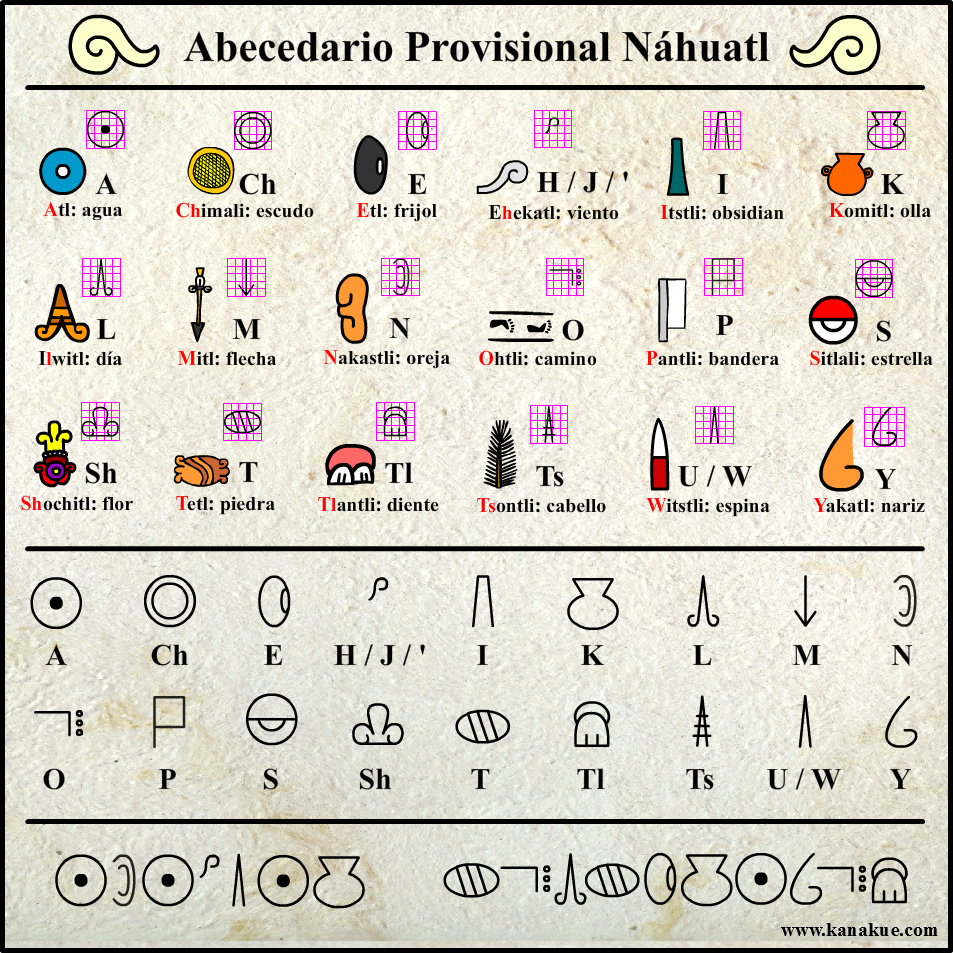
\includegraphics[keepaspectratio]{images/02ebf77bcfe068987b8a9bcc02498d49.png}}

}

\caption{Construcción de un ``alfabeto'' fónico para el náuatl.}

\end{figure}%

\pandocbounded{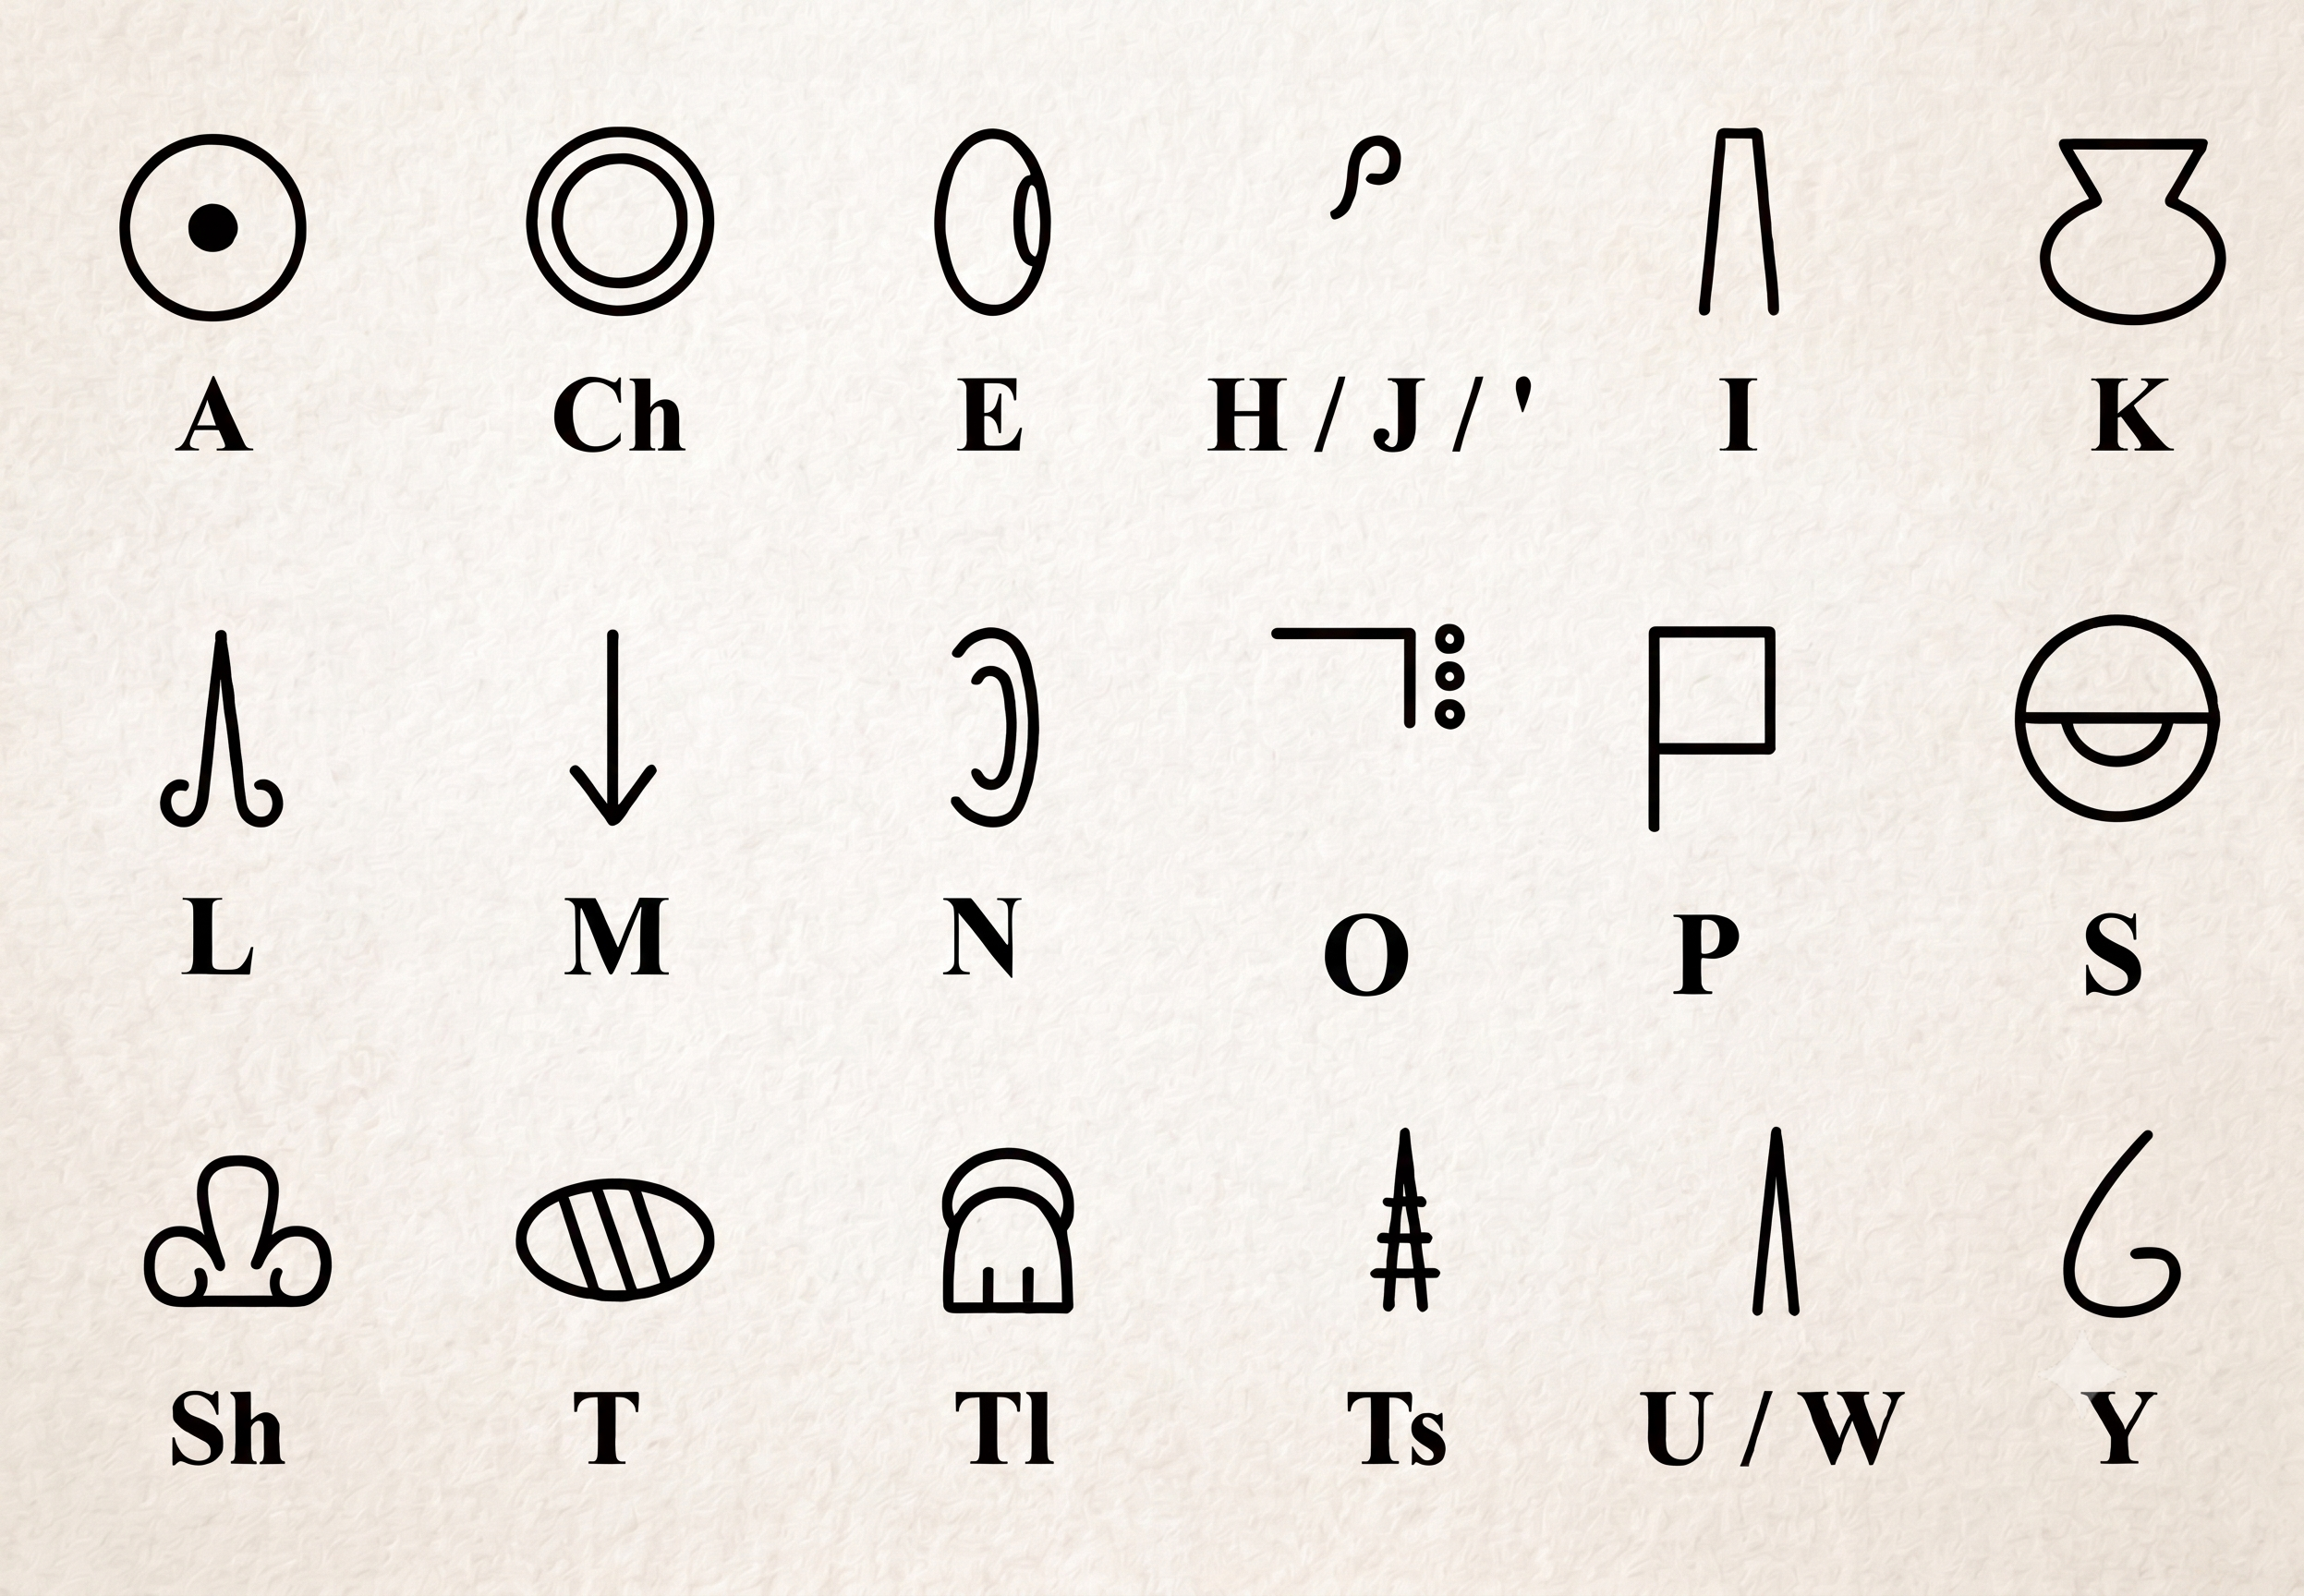
\includegraphics[keepaspectratio]{images/Alfabeto nahuatl.png}}

La preservación de estos documentos y sistemas de escritura no solo
implica su conservación física, sino también su digitalización y
análisis computacional para garantizar su accesibilidad a futuras
generaciones. Sin embargo, este proceso enfrenta un desafío importante:
la transcripción manual por parte de especialistas es un proceso lento,
costoso y propenso a errores. En este contexto, el desarrollo de
herramientas automatizadas de reconocimiento se vuelve crucial.

No obstante, a diferencia de los textos alfabéticos modernos, la
naturaleza particular de estos sistemas de escritura representa un
desafío de modelado matemático y computacional que requiere técnicas
avanzadas de reconocimiento de patrones.

\subsection{El reto del reconocimiento óptico de caracteres en lenguas
indígenas}\label{el-reto-del-reconocimiento-uxf3ptico-de-caracteres-en-lenguas-induxedgenas}

El Reconocimiento Óptico de Caracteres (OCR, por sus siglas en inglés)
ha alcanzado niveles de madurez notables para la digitalización de
textos en lenguas mayoritarias con alfabetos estandarizados, como el
español o el inglés. Sin embargo, su aplicación a sistemas de escritura
indígenas, y particularmente a propuestas como el Abecedario Provisional
Náhuatl, enfrenta desafíos que trascienden la ingeniería de software y
se adentran en el aprendizaje automático.Algunos de estos desafíos son:

\begin{enumerate}
\def\labelenumi{\arabic{enumi}.}
\item
  \textbf{Variabilidad en la representación fonética:} A diferencia de
  un alfabeto estandarizado donde cada sonido tiene una representación
  única, en el náhuatl existe cierta flexibilidad en la elección del
  glifo para representar un fonema. Por ejemplo, para el sonido /e/,
  teóricamente se podría elegir entre el glifo de \emph{etl} (frijol) o
  \emph{elotl} (elote). Esta ambigüedad en el diseño ortográfico
  representa un desafío para la estandarización.
\item
  \textbf{Falta de estandarización tipográfica:} No existe un ``tipo de
  letra'' único para estos sistemas. Cada material educativo, comunidad
  o institución puede emplear ligeras variantes de los símbolos, lo que
  genera una alta variabilidad en las formas geométricas que un sistema
  de reconocimiento debe procesar.
\item
  \textbf{Ausencia de conjuntos de datos públicos:} A diferencia de
  alfabetos como el latino, para los cuales existen repositorios masivos
  y estandarizados (como EMNIST o MNIST), no existen bases de datos
  públicas de glifos náhuatl etiquetados. Esto limita severamente la
  aplicación directa de técnicas modernas de aprendizaje profundo que
  requieren grandes volúmenes de datos.
\item
  \textbf{Variabilidad morfológica en el trazo:} Una vez establecida la
  elección del glifo para un fonema (por ejemplo, decidir que /e/ se
  representa con el glifo de ``frijol''), el sistema debe ser capaz de
  reconocer dicho glifo independientemente de las variaciones en el
  trazo, la escala, la rotación o pequeñas deformaciones que introduzca
  el usuario al dibujarlo.
\end{enumerate}

\textbf{Delimitación del problema de investigación:}

Para abordar este problema desde las matemáticas aplicadas, es necesario
realizar una delimitación clara del alcance. Si bien la variabilidad en
la elección del pictograma (frijol vs.~elote) es un problema lingüístico
relevante, su resolución excede el ámbito de esta tesis.

Por lo tanto, \textbf{este trabajo asume un sistema ortográfico fijo y
estandarizado}: el Abecedario Provisional Náhuatl mostrado en la Figura
@abcnauatl, donde se ha establecido de manera definitiva qué glifo
representa a cada fonema. Bajo esta suposición, el problema se traslada
al terreno del \textbf{reconocimiento de patrones}, el cual presenta
desafíos matemáticos propios que justifican la comparación de dos
enfoques fundamentales:

\begin{itemize}
\item
  \textbf{Modelos Ocultos de Markov (HMM):} Que modelan la secuencia
  estocástica de los rasgos geométricos extraídos del trazo mediante
  procesos probabilísticos.
\item
  \textbf{Redes Neuronales Convolucionales (CNN):} Que aprenden las
  invariantes espaciales y topológicas directamente de la matriz de
  píxeles mediante optimización en espacios tensoriales.
\end{itemize}

La comparación sistemática de estos dos enfoques permitirá determinar
qué arquitectura matemática es más robusta para reconocer los glifos de
este sistema provisional, sentando las bases para futuras herramientas
de digitalización del patrimonio lingüístico náhuatl.

\section{Planteamiento del Problema}\label{planteamiento-del-problema}

El reconocimiento automático de patrones en sistemas de escritura no
estandarizados presenta desafíos que exceden las capacidades de los
algoritmos de reconocimiento óptico de caracteres (OCR) convencionales.
Al centrar el estudio en el ``alfabeto Náhuatl'', el problema de
investigación se formula desde la perspectiva de la modelación
matemática y el aprendizaje automático, identificando dos grandes áreas
de complejidad: la naturaleza morfológica de los glifos y la dicotomía
entre los paradigmas de modelado estocástico y tensorial.

\subsection{Limitaciones de los enfoques tradicionales en glifos con
alta variabilidad
morfológica}\label{limitaciones-de-los-enfoques-tradicionales-en-glifos-con-alta-variabilidad-morfoluxf3gica}

Los sistemas de OCR tradicionales y los modelos de clasificación de
imágenes estándar asumen la existencia de una tipografía subyacente o,
al menos, una geometría rígida y estandarizada para cada clase
(carácter). En el caso del alfabeto latino, la varianza entre distintas
instancias de la misma letra es relativamente baja y puede ser modelada
mediante transformaciones afines simples.

Sin embargo, los glifos del sistema provisional náhuatl poseen una
naturaleza geométrica y pictográfica que rompe estos supuestos. Al no
existir una fuente tipográfica digital oficial, cada instancia de un
glifo (por ejemplo, el símbolo correspondiente a la sílaba ``Tl'')
presenta variaciones significativas en la curvatura, la proporción de
sus componentes y la continuidad de sus trazos.

Matemáticamente, esto se traduce en distribuciones de probabilidad de
las características de la imagen con una varianza intra-clase
extremadamente alta y, en muchos casos, no gaussiana. Los enfoques
tradicionales, que dependen de la correlación de plantillas (template
matching) o de la extracción manual de características geométricas
rígidas, fallan al no poder generalizar sobre esta alta dispersión
morfológica. Además, la degradación natural de los documentos físicos
(ruido de alta frecuencia, manchas, pérdida de contraste) introduce
incertidumbre en los bordes y contornos de los glifos, lo que exige
modelos matemáticos intrínsecamente robustos al ruido y a las
deformaciones locales.

\subsection{La dicotomía matemática: Modelos Generativos Secuenciales
(HMM) vs.~Modelos Discriminativos Tensoriales
(CNN)}\label{la-dicotomuxeda-matemuxe1tica-modelos-generativos-secuenciales-hmm-vs.-modelos-discriminativos-tensoriales-cnn}

Para abordar la alta variabilidad morfológica descrita anteriormente, la
literatura de visión por computadora y reconocimiento de patrones ofrece
dos paradigmas matemáticos fundamentalmente distintos, cada uno con
fortalezas y limitaciones teóricas particulares:

\textbf{1. El enfoque estocástico y secuencial (Modelos Ocultos de
Markov - HMM):} Los HMM modelan el glifo no como una imagen estática,
sino como la realización observable de un proceso estocástico
secuencial. Al proyectar la imagen 2D en una secuencia 1D de
características estructurales (como la distribución de ``tinta'', el
centro de gravedad o las transiciones de bordes), el HMM utiliza
matrices de transición y de emisión para capturar la probabilidad de
evolución del trazo. * \emph{Ventaja matemática:} Poseen una sólida
fundamentación en la teoría de la probabilidad, permiten cuantificar la
incertidumbre y son altamente interpretables (es posible analizar las
probabilidades de transición entre estados). * \emph{Limitación:}
Dependen críticamente de la \emph{ingeniería manual de características}.
La proyección de 2D a 1D conlleva una pérdida irreversible de
información topológica y espacial, y la matriz de emisión sufre la
``maldición de la dimensionalidad'' si el alfabeto de símbolos
observables es demasiado grande.

\textbf{2. El enfoque de optimización en espacios tensoriales (Redes
Neuronales Convolucionales - CNN):} Las CNN abordan el problema desde el
análisis funcional y el álgebra lineal en espacios de alta dimensión. Al
tratar la imagen como un tensor en \(\mathbb{R}^{H \times W \times C}\),
aplican operadores de convolución (productos internos locales) que
aprenden de manera endógena (automática) filtros detectores de
características jerárquicas. * \emph{Ventaja matemática:} Gracias a la
compartición de parámetros y las operaciones de \emph{pooling}, son
naturalmente equivariantes a traslaciones y robustas a pequeñas
deformaciones geométricas, eliminando la necesidad de diseñar
características manuales. * \emph{Limitación:} Funcionan como modelos
``caja negra'' (baja interpretabilidad matemática de sus decisiones
internas) y requieren una gran cantidad de datos para ajustar sus miles
de parámetros mediante descenso de gradiente, evitando el sobreajuste.

\textbf{Formulación del problema de investigación:} Dada la escasez de
datos etiquetados para lenguas indígenas (lo que penaliza a las CNN) y
la complejidad geométrica de los glifos (lo que penaliza a los HMM por
la pérdida de información espacial en la extracción de rasgos), no
existe un consenso teórico sobre qué paradigma es óptimo para este
dominio específico.

Por lo tanto, el problema central de esta tesis es determinar, mediante
un protocolo experimental riguroso, \textbf{cuál de estos dos marcos
matemáticos ---la inferencia probabilística secuencial (HMM) o la
optimización de funciones no lineales en tensores (CNN)--- ofrece un
mejor equilibrio entre precisión de clasificación, eficiencia
computacional e interpretabilidad} para el reconocimiento de los glifos
del alfabeto náhuatl, y bajo qué condiciones morfológicas cada modelo
demuestra su superioridad.

\subsection{Justificación desde las Matemáticas
Aplicadas}\label{justificaciuxf3n-desde-las-matemuxe1ticas-aplicadas}

La elección de comparar Modelos Ocultos de Markov (HMM) y Redes
Neuronales Convolucionales (CNN) para el reconocimiento de los glifos
del alfabeto náhuatl no responde únicamente a tendencias tecnológicas,
sino a la necesidad de evaluar dos paradigmas matemáticos
fundamentalmente distintos para abordar un problema de clasificación de
patrones con alta variabilidad morfológica. Desde la perspectiva de las
matemáticas aplicadas, esta investigación se justifica a través de tres
ejes teóricos principales:

\subsubsection{Inferencia estocástica vs.~Optimización en espacios
tensoriales}\label{inferencia-estocuxe1stica-vs.-optimizaciuxf3n-en-espacios-tensoriales}

El primer paradigma, representado por los HMM, aborda el reconocimiento
de patrones desde la \textbf{teoría de la probabilidad y los procesos
estocásticos}. En este enfoque, el glifo no se trata como un objeto
geométrico estático, sino como la realización observable de un proceso
secuencial. La inferencia del carácter se formula como un problema de
máxima verosimilitud, donde el algoritmo de
\emph{Expectation-Maximization} (Baum-Welch) estima los parámetros de
transición y emisión en un espacio de estados discretos. La fortaleza
matemática de este modelo radica en su rigor probabilístico y su
capacidad para cuantificar la incertidumbre inherente a los trazos
degradados o ambiguos.

El segundo paradigma, representado por las CNN, se fundamenta en el
\textbf{análisis funcional y la optimización no lineal en espacios de
alta dimensión}. Aquí, la imagen se modela como un tensor en
\(\mathbb{R}^{H \times W \times C}\), y el reconocimiento se formula
como la minimización de una función de pérdida (como la entropía
cruzada) mediante el flujo de gradiente (descenso de gradiente
estocástico). La justificación de este enfoque reside en su capacidad
para aproximar funciones no lineales complejas y aprender operadores de
convolución que actúan como detectores de características locales, sin
requerir una modelación explícita de la dinámica subyacente del trazo.

Comparar ambos enfoques permite determinar si, para un sistema de
escritura con alta varianza intra-clase, es más eficiente modelar la
\textbf{dependencia secuencial de los rasgos} (HMM) o aprender la
\textbf{invarianza topológica mediante composiciones de funciones no
lineales} (CNN).

\subsubsection{El tratamiento de la dimensionalidad y la invarianza
geométrica}\label{el-tratamiento-de-la-dimensionalidad-y-la-invarianza-geomuxe9trica}

Un aspecto crucial en el reconocimiento de los glifos náhuatl es cómo
cada modelo matemático gestiona la dimensionalidad de la entrada y las
transformaciones geométricas.

Los HMM requieren una proyección del espacio bidimensional de la imagen
(\(\mathbb{R}^{28 \times 28}\)) a una secuencia unidimensional de
características discretas (\(\mathbb{R}^T\)). Matemáticamente, esta
reducción de dimensionalidad conlleva una pérdida irreversible de
información espacial y topológica, obligando al modelo a depender
críticamente de la ingeniería manual de características (como el cálculo
de momentos, perfiles y transiciones).

Por el contrario, las CNN operan directamente sobre el tensor de la
imagen, preservando la estructura espacial local. Gracias a la propiedad
de equivarianza por traslación inducida por la compartición de
parámetros en los kernels convolucionales, y a la invarianza aproximada
proporcionada por las operaciones de \emph{pooling}, las CNN manejan las
deformaciones geométricas (rotaciones, traslaciones y escalados) de
manera endógena. Evaluar el impacto de estas dos estrategias de manejo
de la dimensionalidad es esencial para entender los límites de cada
modelo frente a la falta de estandarización tipográfica de los glifos.

\subsubsection{Interpretabilidad matemática y escasez de
datos}\label{interpretabilidad-matemuxe1tica-y-escasez-de-datos}

Finalmente, la investigación se justifica por la naturaleza del conjunto
de datos. Al tratarse de un sistema de escritura indígena, no existen
repositorios masivos de datos etiquetados, lo que impone un escenario de
\textbf{aprendizaje con datos limitados}.

Los modelos probabilísticos como los HMM, al tener un espacio de
parámetros mucho más restringido (matrices de transición y emisión) y
estar guiados por supuestos estructurales fuertes (como la topología de
Bakis para secuencias unidireccionales), suelen ser más robustos ante la
escasez de datos y ofrecen una \textbf{interpretabilidad matemática
directa}: es posible analizar las probabilidades de transición entre
estados para entender cómo el modelo ``decide'' la clase.

En contraste, las CNN poseen miles de parámetros ajustables, lo que las
hace propensas al sobreajuste en escenarios de pocos datos, requiriendo
técnicas de regularización (como \emph{Dropout} o \emph{Weight Decay}) y
aumentación de datos sintéticos. Además, su naturaleza de ``caja negra''
dificulta la interpretación de las decisiones internas.

Por lo tanto, esta tesis aporta valor a las matemáticas aplicadas al
cuantificar formalmente el equilibrio entre \textbf{precisión, costo
computacional, robustez ante datos limitados e interpretabilidad},
estableciendo un precedente metodológico para el procesamiento
computacional de lenguas originarias y sistemas de escritura no
estandarizados. \#\# 1.4 Objetivos

\subsection{Objetivo General}\label{objetivo-general}

Comparar el desempeño de los Modelos Ocultos de Markov (HMM) con esquema
de remuestreo \emph{bootstrap} y las Redes Neuronales Convolucionales
(CNN) en la clasificación de imágenes monocromáticas de glifos del
alfabeto náhuatl. Dicha comparación se realizará mediante la
implementación de ambos algoritmos bajo un protocolo experimental
estandarizado, con el fin de determinar cuál enfoque ofrece el mejor
equilibrio entre precisión de clasificación, costo computacional e
interpretabilidad matemática para el reconocimiento automático de
patrones.

\subsection{Objetivos Particulares}\label{objetivos-particulares}

Para alcanzar el objetivo general, se plantean los siguientes objetivos
particulares:

\begin{enumerate}
\def\labelenumi{\arabic{enumi}.}
\item
  \textbf{Preprocesar y caracterizar el conjunto de datos} de imágenes
  monocromáticas de glifos del alfabeto náhuatl, aplicando técnicas de
  normalización, aumentación geométrica y generación de ruido
  controlado, para establecer una base de evaluación estandarizada y
  robusta que permita la comparación equitativa de ambos modelos.
\item
  \textbf{Implementar y ajustar un modelo de clasificación basado en
  Modelos Ocultos de Markov (HMM)} categóricos, integrado con un esquema
  de remuestreo \emph{bootstrap}. El propósito es modelar la secuencia
  de características estructurales extraídas de los glifos y cuantificar
  la incertidumbre estadística en su identificación.
\item
  \textbf{Diseñar y entrenar una arquitectura de Red Neuronal
  Convolucional (CNN)} optimizada para imágenes de baja resolución,
  formulando adecuadamente la función de pérdida y el proceso de
  optimización (ej. Adam), para extraer características espaciales
  jerárquicas y maximizar la precisión en la clasificación de las
  distintas clases de glifos.
\item
  \textbf{Evaluar y comparar el rendimiento de ambos enfoques} (HMM y
  CNN) mediante métricas de desempeño (exactitud, precisión,
  exhaustividad y función de pérdida), tiempos de convergencia y
  requerimientos de recursos computacionales, para identificar las
  ventajas, limitaciones y el ámbito de aplicabilidad de cada método en
  el contexto del reconocimiento de patrones glíficos.
\end{enumerate}

\bookmarksetup{startatroot}

\chapter{Fundamentos CNN}\label{fundamentos-cnn}

En este trabajo se aborda el problema de \textbf{reconocimiento
automático de glifos del alfabeto náhuatl} mediante el uso de redes
neuronales convolucionales (\emph{Convolutional Neural Networks}, CNN).
Este problema puede formularse como una tarea de clasificación de
imágenes, en la cual cada glifo es representado mediante una estructura
matricial que codifica su información visual.

Los glifos presentan variaciones en forma, trazo y estilo, lo que
dificulta su identificación mediante métodos tradicionales. En este
contexto, las CNN resultan particularmente adecuadas debido a su
capacidad para extraer características espaciales relevantes
directamente a partir de los datos, tales como bordes, curvas y patrones
geométricos distintivos.

\bookmarksetup{startatroot}

\chapter{Formulación Matemática de una
CNN}\label{formulaciuxf3n-matemuxe1tica-de-una-cnn}

Una red neuronal convolucional puede modelarse como una aplicación
parametrizada:

\begin{equation}\phantomsection\label{eq-cnn-formal}{
f(\cdot , \theta): \mathcal{X} \subseteq \mathbb{R}^{H \times W \times C} \longrightarrow \mathbb{R}^{k}
}\end{equation}

donde:

\begin{itemize}
\tightlist
\item
  \(\mathcal{X}\) es el espacio de entrada (por ejemplo, imágenes),
\item
  \(H\) representa la altura (height) de la imagen, es decir, el número
  de filas,
\item
  \(W\) representa el ancho (width), es decir, el número de columnas,
\item
  \(C\) representa el número de canales (channels), que corresponde a la
  cantidad de valores asociados a cada píxel,
\item
  \(k\) es la dimensión del espacio de salida (por ejemplo, número de
  clases en clasificación),
\item
  \(\theta\) denota el conjunto total de parámetros entrenables del
  modelo.
\end{itemize}

\bookmarksetup{startatroot}

\chapter{Representación Tensorial de
Imágenes}\label{representaciuxf3n-tensorial-de-imuxe1genes}

Una imagen digital se representa como un tensor de orden tres:

\begin{equation}\phantomsection\label{eq-imagen-tensor}{
X \in \mathbb{R}^{H \times W \times C}
}\end{equation}

Esto implica que para cada posición espacial \((i,j)\):

\begin{equation}\phantomsection\label{eq-pixel-vector}{
X(i,j) = \left(x_1, x_2, \dots, x_C \right) \in \mathbb{R}^C
}\end{equation}

Por tanto, cada píxel contiene un vector que describe información en
distintos canales.

\pandocbounded{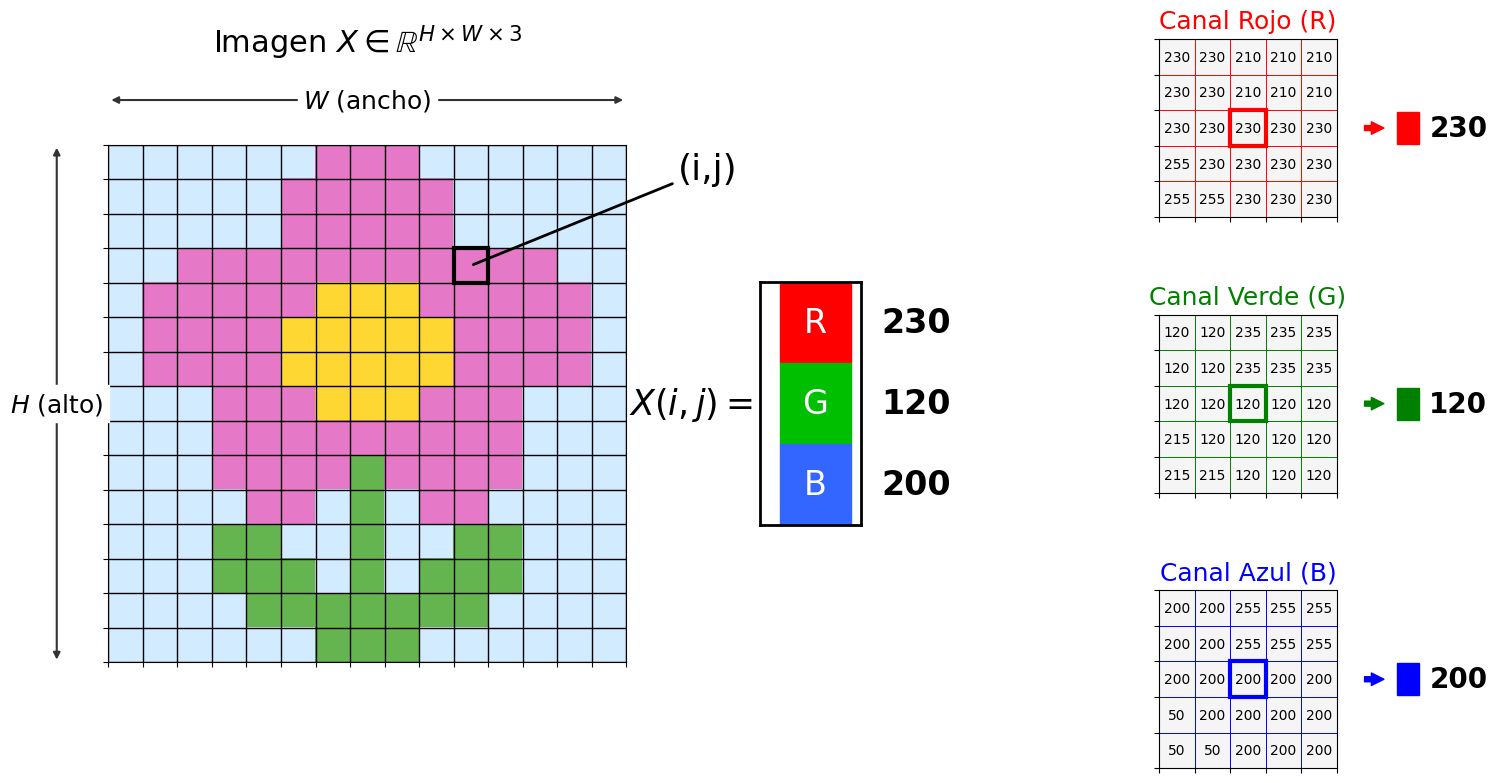
\includegraphics[keepaspectratio]{Imagenes_tesis/Imagen flor 1 corregida.png}}

\bookmarksetup{startatroot}

\chapter{Estructura Funcional de la
Red}\label{estructura-funcional-de-la-red}

Una CNN se construye como la composición de funciones:

\begin{equation}\phantomsection\label{eq-composicion-cnn}{
f(x;\theta) = f^{(L)} \circ f^{(L-1)} \circ \cdots \circ f^{(1)}(x)
}\end{equation}

donde \(L \in \mathbb{N}\) es el número total de capas de la red y cada
\(f^{(l)}\) representa una transformación asociada a la capa
\(l\)-ésima.

Asimismo, los parámetros globales se expresan como:

\begin{equation}\phantomsection\label{eq-parametros-globales}{
\theta = \left\{ \theta^{(1)}, \theta^{(2)}, \dots, \theta^{(L)} \right\}
}\end{equation}

\bookmarksetup{startatroot}

\chapter{Parámetros del Modelo}\label{paruxe1metros-del-modelo}

Los parámetros de una CNN están constituidos principalmente por:

\begin{itemize}
\tightlist
\item
  \textbf{Kernels} (filtros convolucionales),
\item
  \textbf{Sesgos} asociados a cada filtro.
\end{itemize}

Estos parámetros determinan completamente la función \(f(x;\theta)\) y
son ajustados mediante procedimientos de optimización basados en
gradiente.

\bookmarksetup{startatroot}

\chapter{Kernels Convolucionales}\label{kernels-convolucionales}

\section{Definición Formal}\label{definiciuxf3n-formal}

Un kernel es un tensor de parámetros que define un operador lineal
local.

\textbf{Caso unicanal:}

\begin{equation}\phantomsection\label{eq-kernel-unicanal}{
K \in \mathbb{R}^{k_h \times k_w}
}\end{equation}

cuyos elementos se indexan como:

\[
K(u,v), \quad
u \in \{0,\dots,k_h-1\}, \;
v \in \{0,\dots,k_w-1\}
\]

\textbf{Caso multicanal:}

\begin{equation}\phantomsection\label{eq-kernel-multicanal}{
K \in \mathbb{R}^{k_h \times k_w \times C}
}\end{equation}

con entradas:

\[
K(u,v,c), \quad
u \in \{0,\dots,k_h-1\}, \;
v \in \{0,\dots,k_w-1\}, \;
c \in \{1,\dots,C\}
\]

\section{Interpretación
Geométrica}\label{interpretaciuxf3n-geomuxe9trica}

Sea \(X_{(i,j)}\) una subregión de la imagen obtenida al centrar el
kernel en la posición \((i,j)\), cuyos elementos están dados por:

\[
X(i+u, j+v, c)
\]

para los mismos índices \((u,v,c)\) definidos anteriormente.

El producto interno:

\begin{equation}\phantomsection\label{eq-producto-interno}{
\langle K, X_{(i,j)} \rangle
}\end{equation}

mide la similitud entre el patrón definido por el kernel y la región
local de la imagen.

\pandocbounded{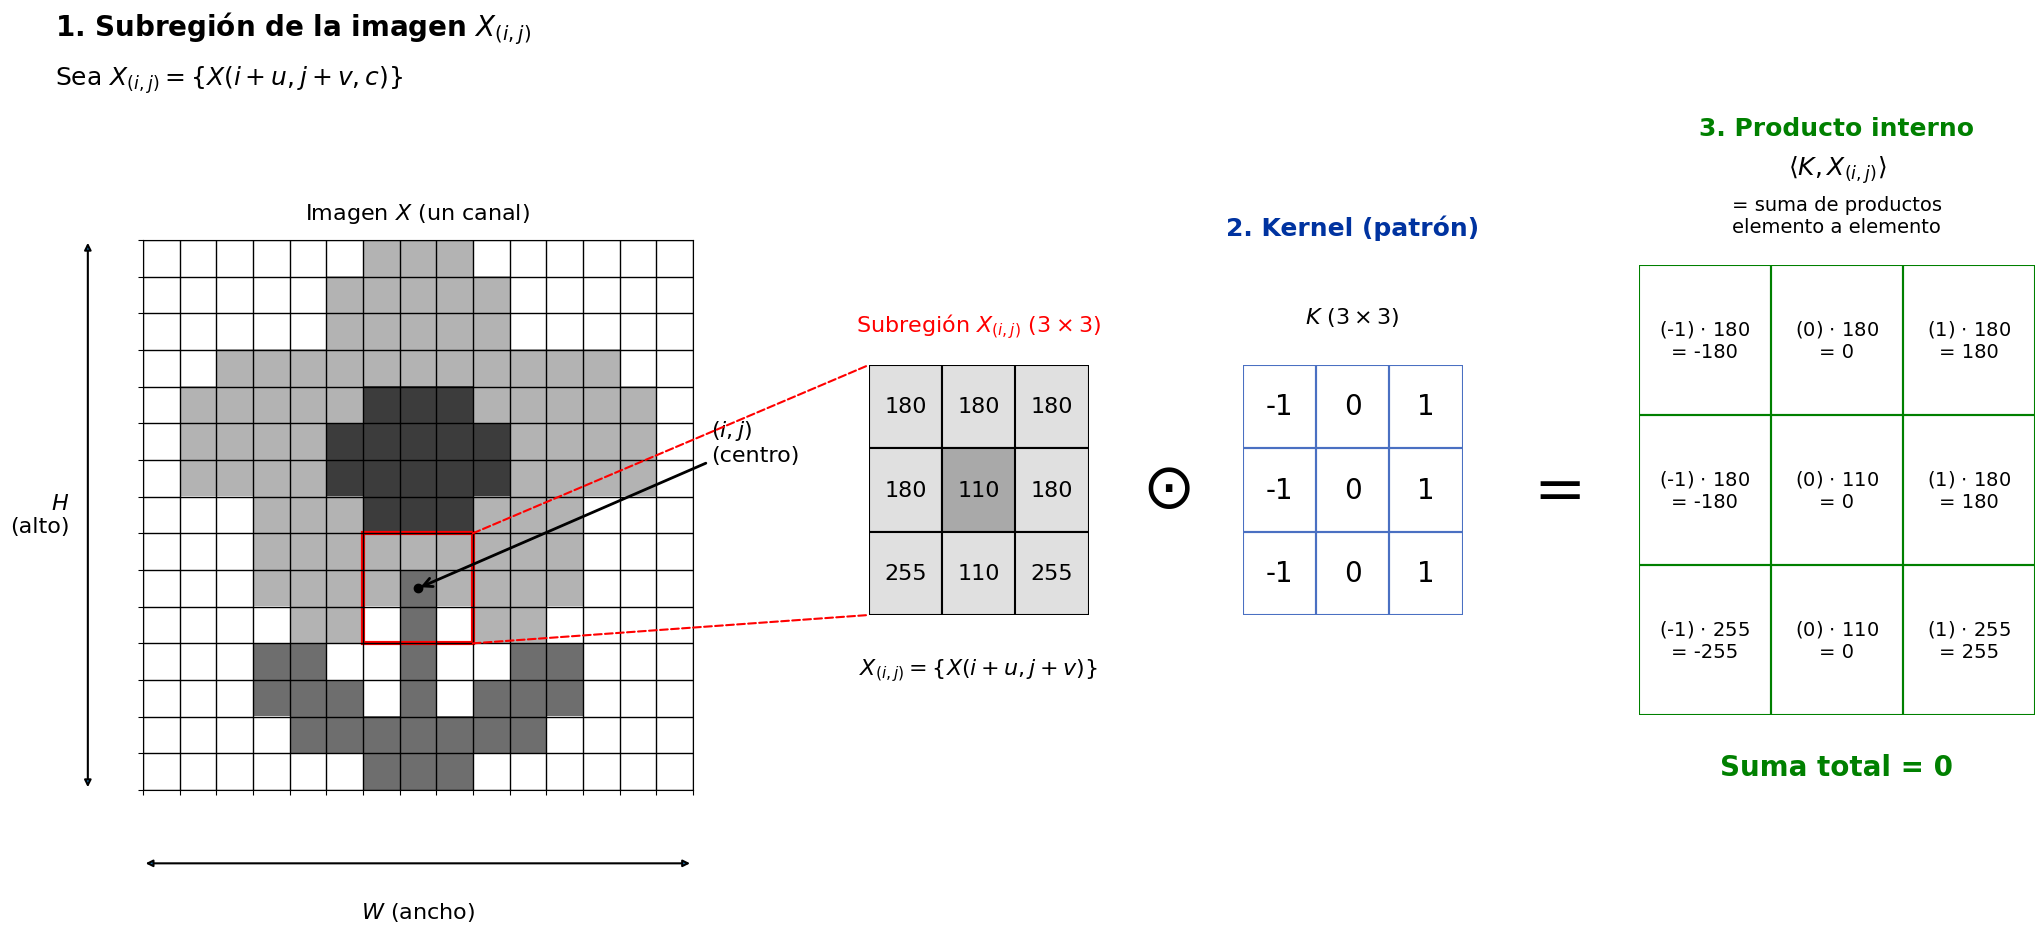
\includegraphics[keepaspectratio]{images/paste-1.png}}

\section{Compartición de
parámetros}\label{comparticiuxf3n-de-paruxe1metros}

Una propiedad fundamental de las redes neuronales convolucionales es la
\textbf{compartición de parámetros}, la cual establece que los
coeficientes del kernel no dependen de la posición espacial en la que se
aplica la operación.

Formalmente, si \(K\) es un kernel convolucional, entonces:

\[
K(u,v,c) \text{ es independiente de la posición } (i,j)
\]

Esto implica que el mismo kernel es utilizado para procesar todas las
regiones locales de la entrada.

\subsection{Reducción del número de
parámetros}\label{reducciuxf3n-del-nuxfamero-de-paruxe1metros}

En ausencia de compartición de parámetros, cada posición \((i,j)\)
requeriría un conjunto distinto de pesos, lo cual conduciría a un número
total de parámetros del orden:

\[
H \cdot W \cdot k_h \cdot k_w \cdot C
\]

Sin embargo, al emplear un único kernel compartido, el número de
parámetros se reduce a:

\[
k_h \cdot k_w \cdot C
\]

lo cual representa una reducción significativa en la complejidad del
modelo.

\subsection{Invarianza traslacional}\label{invarianza-traslacional}

La compartición de parámetros induce una propiedad de
\textbf{equivarianza por traslación}. Sea \(\tau_{a,b}\) un operador de
traslación definido sobre la entrada. Entonces, la operación de
convolución satisface:

\begin{equation}\phantomsection\label{eq-equivarianza}{
\mathcal{T}_K(\tau_{a,b} X) = \tau_{a,b} (\mathcal{T}_K X)
}\end{equation}

Esto implica que si una característica aparece en diferentes posiciones
espaciales, el modelo será capaz de detectarla de manera consistente.

En consecuencia, la red no depende de la posición absoluta de los
patrones, sino únicamente de su estructura local.

\bookmarksetup{startatroot}

\chapter{Operación de Convolución}\label{operaciuxf3n-de-convoluciuxf3n}

La operación fundamental en una red neuronal convolucional es la
denominada \textbf{convolución discreta}. No obstante, es importante
señalar que en el contexto de aprendizaje profundo, la operación
implementada corresponde en realidad a la \textbf{correlación cruzada},
ya que no se realiza la inversión del kernel. A pesar de esta diferencia
técnica, en la literatura se mantiene el término ``convolución'\,' por
convención.

Esta operación define un mecanismo mediante el cual se evalúa la
similitud entre un patrón local (kernel) y distintas regiones de la
imagen de entrada.

\section{Caso Unicanal}\label{caso-unicanal}

Sea una imagen unicanal representada por:

\[
X \in \mathbb{R}^{H \times W}
\]

y un kernel:

\[
K \in \mathbb{R}^{k_h \times k_w}
\]

La operación de convolución produce una salida \(Y\), definida en cada
posición \((i,j)\) como:

\begin{equation}\phantomsection\label{eq-convolucion-unicanal}{
Y(i,j) =
\sum_{u=0}^{k_h-1}
\sum_{v=0}^{k_w-1}
K(u,v)\, X(i+u, j+v)
}\end{equation}

donde:

\begin{itemize}
\tightlist
\item
  \((i,j)\) denota la posición de la ventana deslizante,
\item
  \((u,v)\) recorre las coordenadas internas del kernel,
\item
  \(X(i+u, j+v)\) representa la región local de la imagen.
\end{itemize}

\pandocbounded{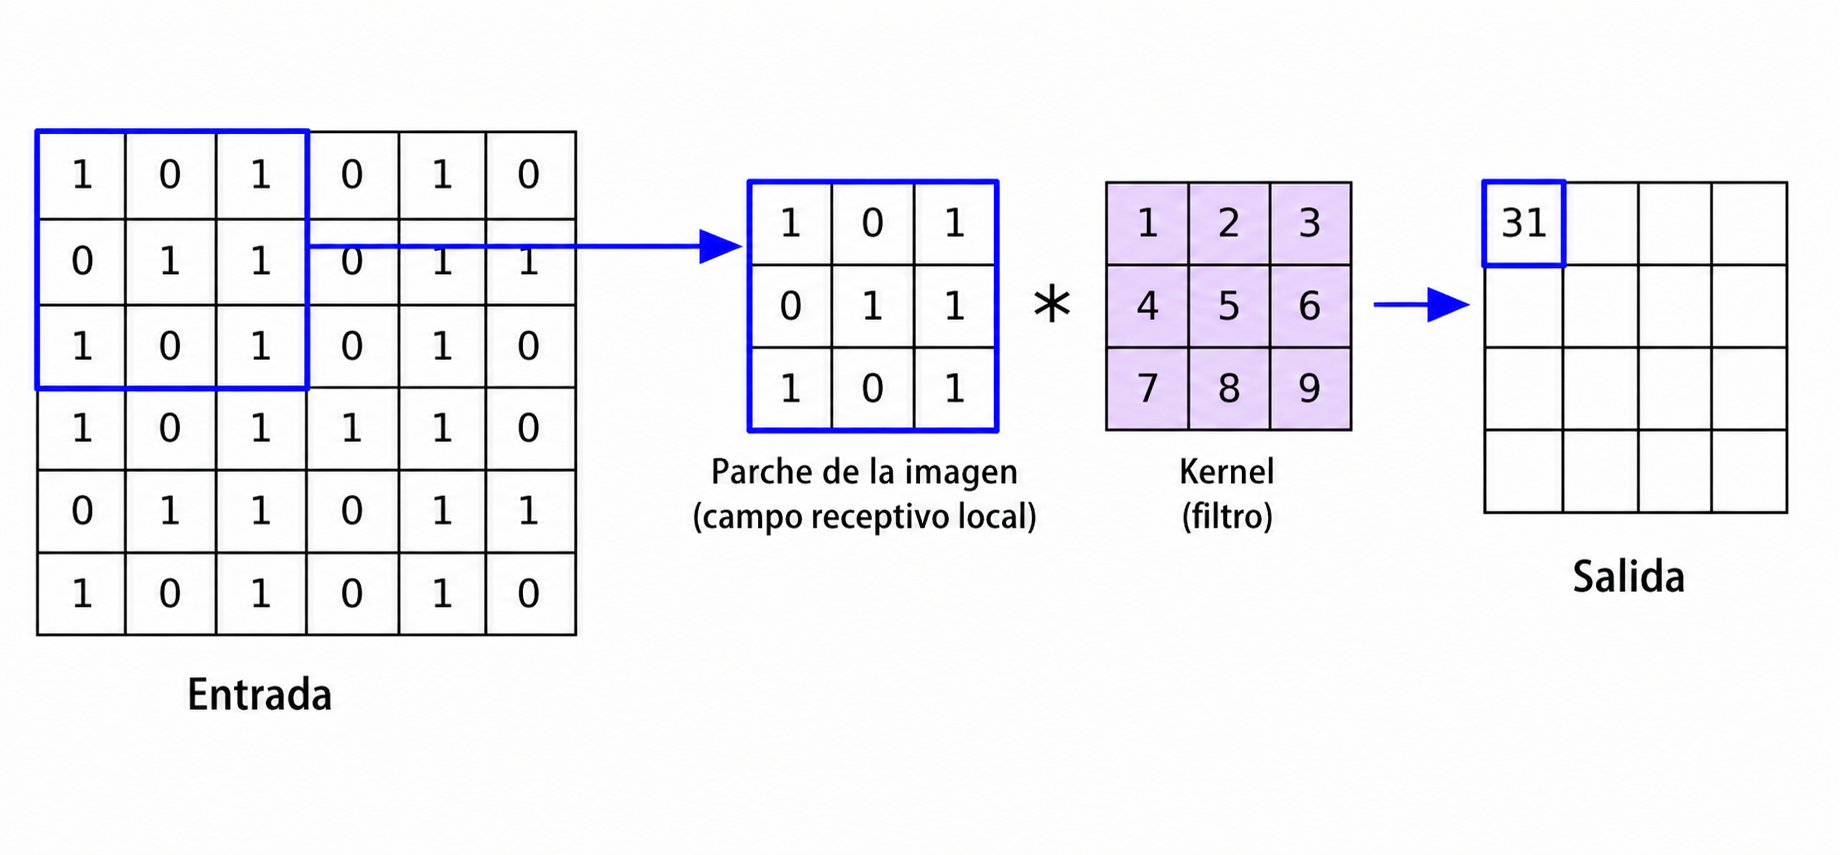
\includegraphics[keepaspectratio]{Imagenes_tesis/img_kernel_1.png}}

\subsection{Interpretación como ventana
deslizante}\label{interpretaciuxf3n-como-ventana-deslizante}

La ecuación anterior describe un proceso en el cual el kernel se
desplaza sistemáticamente sobre la imagen. En cada posición, se
selecciona una submatriz de \(X\) de dimensiones \(k_h \times k_w\),
sobre la cual se realiza una operación de agregación ponderada.

Formalmente, definimos la submatriz local como:

\[
X_{(i,j)} = \left\{ X(i+u, j+v) \right\}_{u,v}
\]

Por lo tanto, la salida en \((i,j)\) depende únicamente de una vecindad
local de la imagen, lo cual establece la propiedad de
\textbf{conectividad local}.

\subsection{Interpretación como producto
interno}\label{interpretaciuxf3n-como-producto-interno}

La expresión de la convolución puede reescribirse como un producto
interno en el espacio vectorial \(\mathbb{R}^{k_h \times k_w}\):

\begin{equation}\phantomsection\label{eq-producto-interno-conv}{
Y(i,j) = \langle K, X_{(i,j)} \rangle
}\end{equation}

donde el producto interno se define como:

\[
\langle A, B \rangle = \sum_{u=0}^{k_h-1} \sum_{v=0}^{k_w-1} A(u,v)\, B(u,v)
\]

Esta formulación pone de manifiesto que la convolución mide el grado de
alineación entre el kernel y la región local.

\subsection{Interpretación
geométrica}\label{interpretaciuxf3n-geomuxe9trica-1}

Desde un punto de vista geométrico, el valor \(Y(i,j)\) representa la
proyección del vector \(X_{(i,j)}\) sobre el vector \(K\) en el espacio
euclidiano de dimensión \(k_h k_w\). En consecuencia:

\begin{itemize}
\tightlist
\item
  Si \(X_{(i,j)}\) es similar a \(K\), entonces \(Y(i,j)\) será grande.
\item
  Si son ortogonales, el resultado será cercano a cero.
\item
  Si son opuestos, el valor será negativo.
\end{itemize}

Esto permite interpretar al kernel como un \textbf{detector de
patrones}.

\subsection{Naturaleza lineal de la
operación}\label{naturaleza-lineal-de-la-operaciuxf3n}

La convolución es un operador lineal. Es decir, para cualesquiera
tensores \(X_1, X_2\) y escalares \(\alpha, \beta\), se cumple:

\begin{equation}\phantomsection\label{eq-linealidad}{
\mathcal{T}_K(\alpha X_1 + \beta X_2)
= \alpha \mathcal{T}_K(X_1) + \beta \mathcal{T}_K(X_2)
}\end{equation}

donde \(\mathcal{T}_K\) denota el operador de convolución asociado al
kernel \(K\).

\subsection{Relación con la correlación
cruzada}\label{relaciuxf3n-con-la-correlaciuxf3n-cruzada}

Es importante destacar que la definición utilizada en redes neuronales
corresponde a la correlación cruzada:

\[
Y(i,j) =
\sum_{u,v} K(u,v)\, X(i+u, j+v)
\]

mientras que la convolución clásica implicaría una inversión del kernel:

\[
Y(i,j) =
\sum_{u,v} K(u,v)\, X(i-u, j-v)
\]

Sin embargo, dado que los parámetros del kernel son aprendidos durante
el entrenamiento, ambas formulaciones resultan equivalentes en términos
de capacidad representacional.

\subsection{Dependencia local}\label{dependencia-local}

Finalmente, se observa que:

\[
Y(i,j) \text{ depende únicamente de } X_{(i,j)}
\]

lo cual implica que cada salida está influenciada únicamente por una
región local de la entrada. Esta propiedad es clave para la eficiencia
computacional y la capacidad de generalización del modelo.

\section{Convolución Multicanal}\label{convoluciuxf3n-multicanal}

En el caso general, las imágenes no son unicanal, sino que poseen
múltiples canales (por ejemplo, RGB). En consecuencia, la operación de
convolución debe extenderse para considerar simultáneamente la
información presente en cada canal.

Sea:

\[
X \in \mathbb{R}^{H \times W \times C}
\]

una imagen con \(C\) canales, y sea un kernel:

\[
K \in \mathbb{R}^{k_h \times k_w \times C}
\]

donde cada canal del kernel corresponde a un canal de la entrada.

La salida de la convolución en la posición \((i,j)\) está dada por:

\begin{equation}\phantomsection\label{eq-convolucion-multicanal}{
Y(i,j) =
\sum_{c=1}^{C}
\sum_{u=0}^{k_h-1}
\sum_{v=0}^{k_w-1}
K(u,v,c)\, X(i+u,j+v,c)
}\end{equation}

Esta expresión indica que la contribución de cada canal se calcula de
manera independiente y posteriormente se agregan (suman) todas las
contribuciones.

La operación anterior puede interpretarse como la suma de convoluciones
unicanal:

\[
Y(i,j) = \sum_{c=1}^{C} Y^{(c)}(i,j)
\]

donde:

\[
Y^{(c)}(i,j) =
\sum_{u=0}^{k_h-1}
\sum_{v=0}^{k_w-1}
K(u,v,c)\, X(i+u,j+v,c)
\]

Cada término \(Y^{(c)}(i,j)\) representa la contribución del canal \(c\)
al valor final de la salida.

\pandocbounded{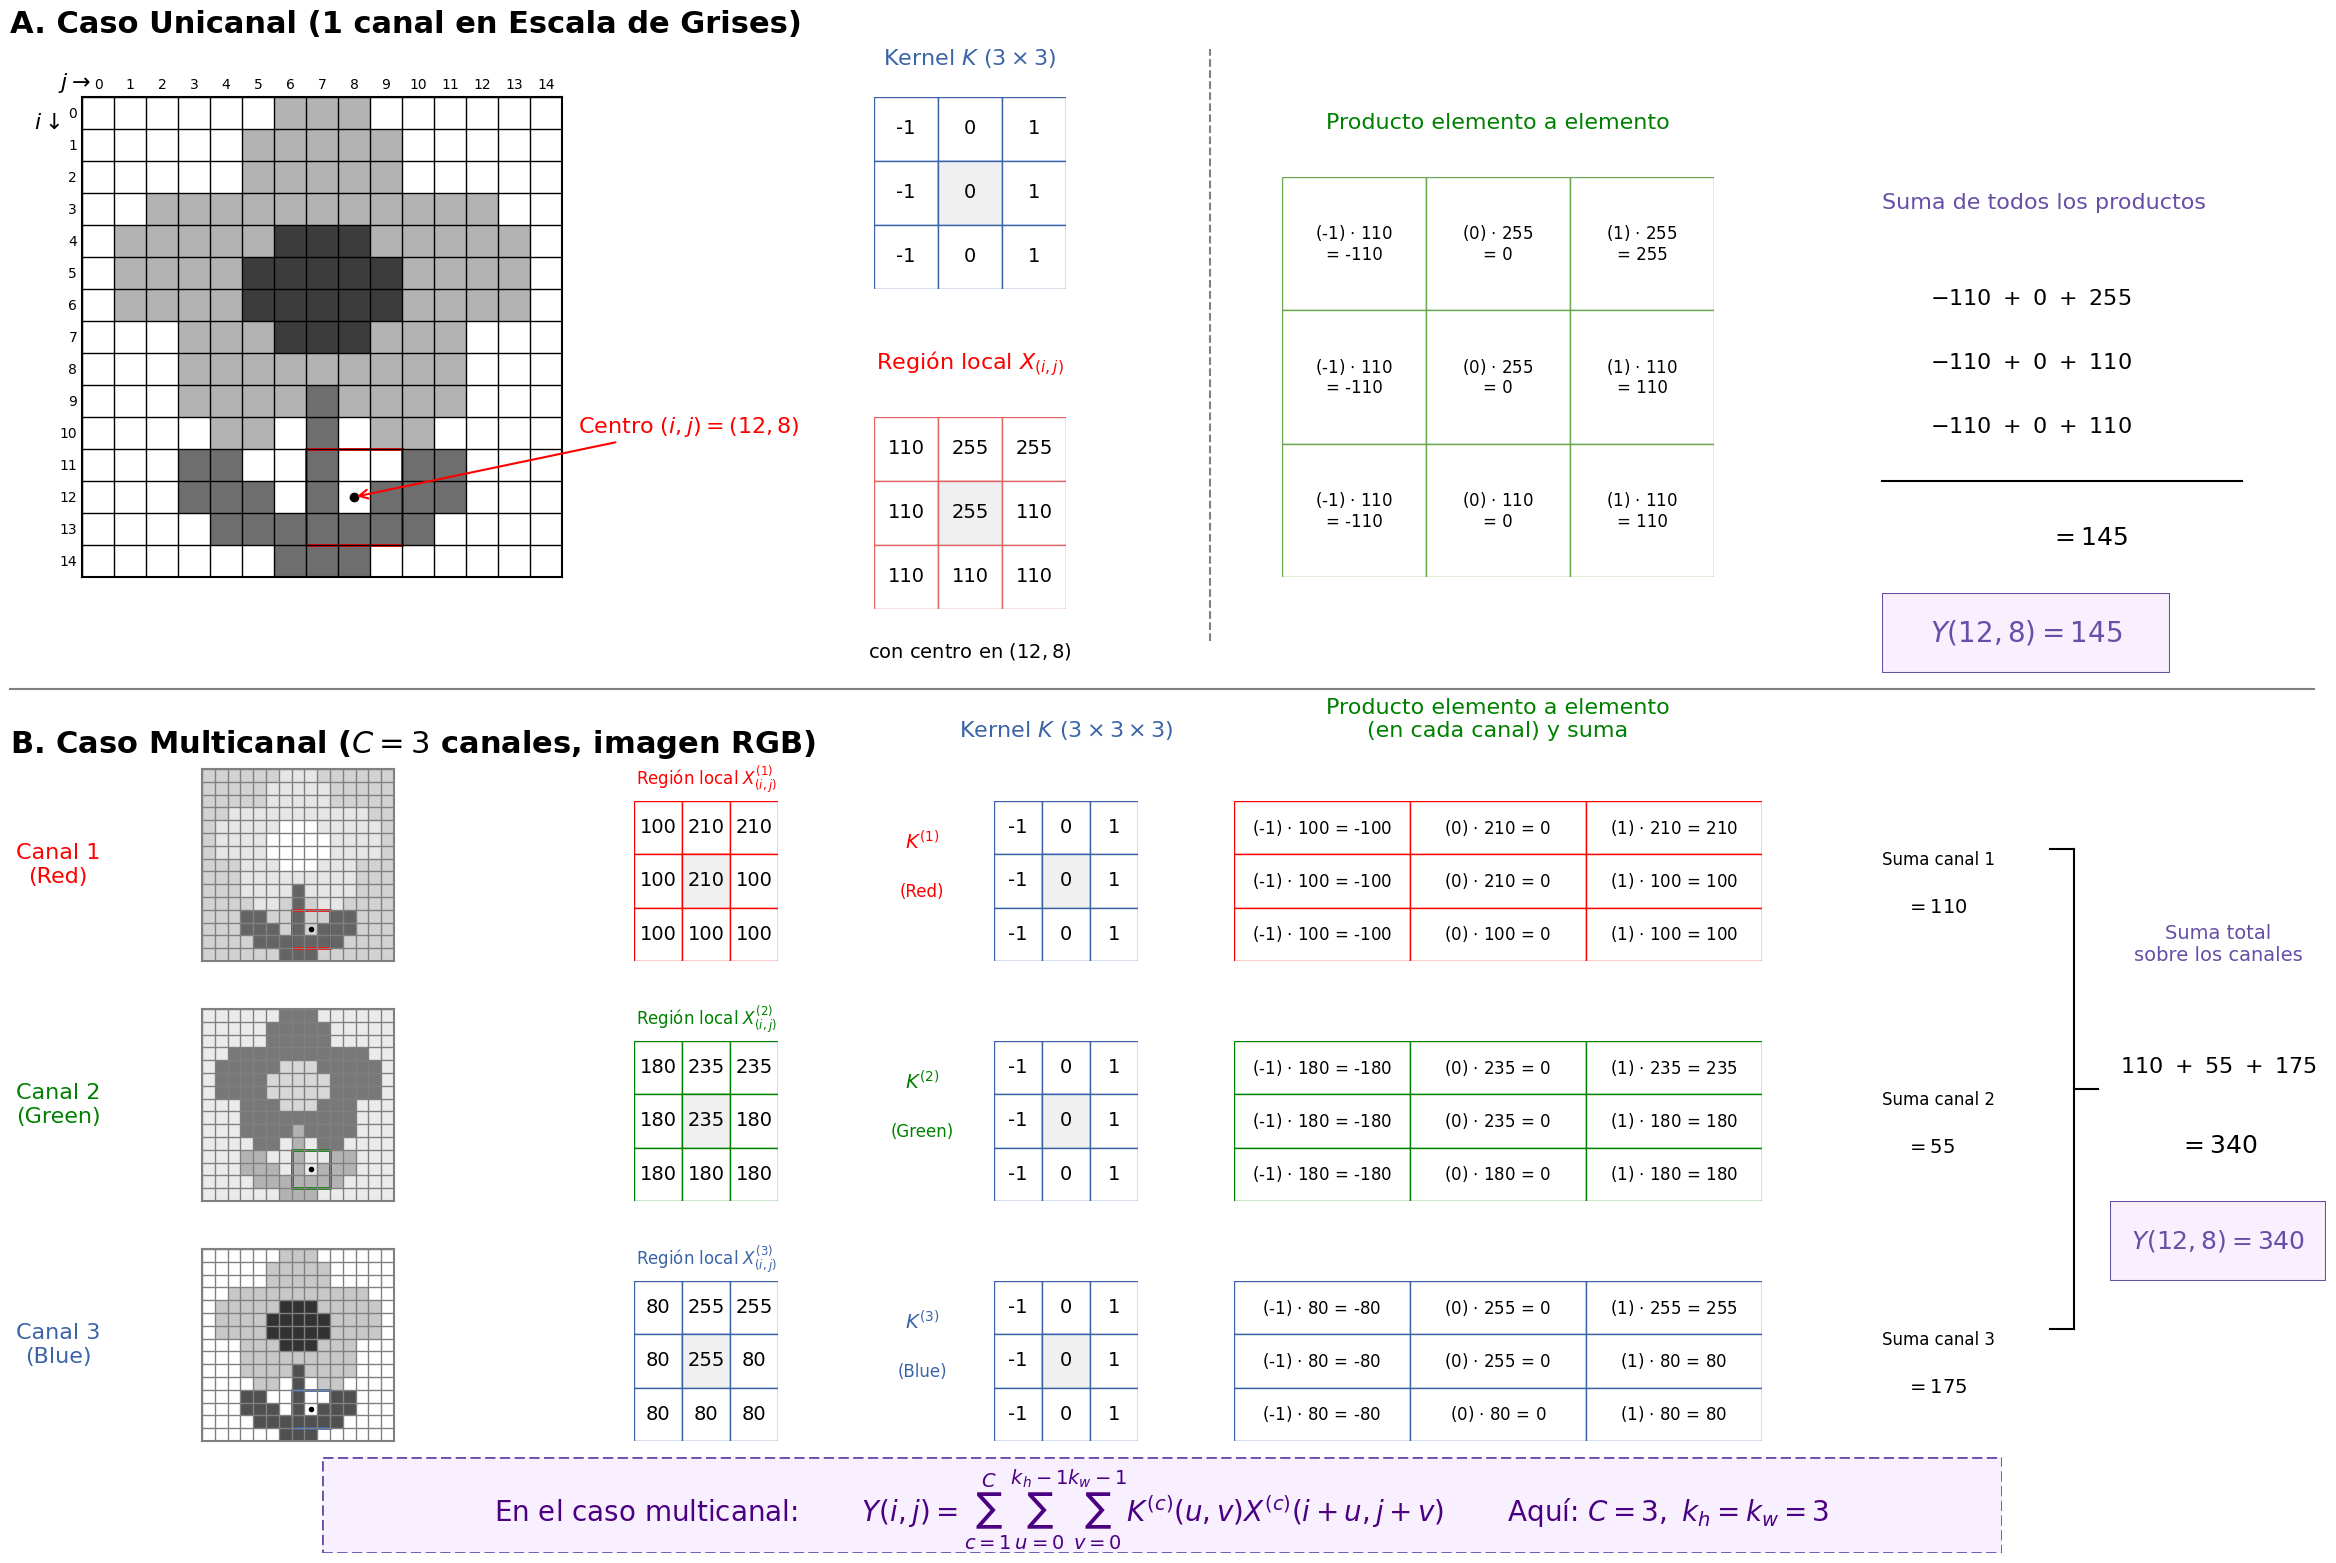
\includegraphics[keepaspectratio]{images/paste-2.png}}

\section{Interpretación como producto interno en espacio
tensorial}\label{interpretaciuxf3n-como-producto-interno-en-espacio-tensorial}

Sea \(X_{(i,j)}\) la subregión local de la imagen centrada en \((i,j)\).
Entonces:

\[
X_{(i,j)} \in \mathbb{R}^{k_h \times k_w \times C}
\]

Al vectorizar ambos tensores:

\[
\mathrm{vec}(X_{(i,j)}) \in \mathbb{R}^{k_h k_w C}, \quad
\mathrm{vec}(K) \in \mathbb{R}^{k_h k_w C}
\]

la convolución puede escribirse como:

\begin{equation}\phantomsection\label{eq-vectorizacion}{
Y(i,j) = \mathrm{vec}(K)^\top \mathrm{vec}(X_{(i,j)})
}\end{equation}

Esto muestra que la operación es un producto interno en un espacio
euclidiano de dimensión \(k_h k_w C\).

\section{Interpretación
geométrica}\label{interpretaciuxf3n-geomuxe9trica-2}

Desde un punto de vista geométrico, cada región local de la imagen se
interpreta como un punto en el espacio \(\mathbb{R}^{k_h k_w C}\), y el
kernel define una dirección en dicho espacio.

Por tanto:

\begin{itemize}
\tightlist
\item
  valores grandes de \(Y(i,j)\) indican alta alineación entre el patrón
  y la región,
\item
  valores cercanos a cero indican baja correlación,
\item
  valores negativos indican oposición estructural.
\end{itemize}

En consecuencia, el kernel actúa como un detector de patrones
multicanal.

\section{Naturaleza lineal}\label{naturaleza-lineal}

La convolución multicanal es un operador lineal. Es decir, para
cualesquiera tensores \(X_1, X_2\) y escalares \(\alpha, \beta\), se
cumple:

\[
\mathcal{T}_K(\alpha X_1 + \beta X_2)
=
\alpha \mathcal{T}_K(X_1) + \beta \mathcal{T}_K(X_2)
\]

donde \(\mathcal{T}_K\) denota el operador de convolución asociado al
kernel \(K\).

\section{Interpretación
estructural}\label{interpretaciuxf3n-estructural}

Es importante destacar que, a diferencia del caso unicanal, el kernel
multicanal no detecta únicamente patrones espaciales, sino también
\textbf{correlaciones entre canales}.

Por ejemplo, en imágenes RGB, el kernel puede aprender a identificar
combinaciones específicas de intensidades en los canales rojo, verde y
azul, lo cual permite detectar patrones más complejos que aquellos
basados únicamente en estructura espacial.

\section{Forma Vectorizada}\label{forma-vectorizada}

\[
Y(i,j) = K^\top X_{(i,j)}
\]

\bookmarksetup{startatroot}

\chapter{Múltiples Filtros}\label{muxfaltiples-filtros}

En una red neuronal convolucional, no se utiliza un único kernel, sino
un conjunto de filtros que permiten extraer distintas características de
la entrada. Este conjunto se denota como:

\begin{equation}\phantomsection\label{eq-conjunto-filtros}{
\left\{ K^{(f)} \right\}_{f=1}^{F}, \quad
K^{(f)} \in \mathbb{R}^{k_h \times k_w \times C}
}\end{equation}

donde \(F\) representa el número total de filtros.

\section{Definición de la salida}\label{definiciuxf3n-de-la-salida}

Cada filtro \(K^{(f)}\) actúa de manera independiente sobre la entrada y
produce un mapa de activación asociado. Para cada posición \((i,j)\), la
salida correspondiente al filtro \(f\) está dada por:

\begin{equation}\phantomsection\label{eq-salida-filtro}{
Y_f(i,j) = \langle K^{(f)}, X_{(i,j)} \rangle
}\end{equation}

Por lo tanto, a cada filtro le corresponde una función:

\[
Y_f : \{1,\dots,H'\} \times \{1,\dots,W'\} \to \mathbb{R}
\]

\section{Estructura tensorial de la
salida}\label{estructura-tensorial-de-la-salida}

Al considerar todos los filtros simultáneamente, la salida completa se
organiza como un tensor de orden tres:

\begin{equation}\phantomsection\label{eq-salida-tensor}{
Y \in \mathbb{R}^{H' \times W' \times F}
}\end{equation}

donde:

\begin{itemize}
\tightlist
\item
  \(H'\) y \(W'\) son las dimensiones espaciales de la salida,
\item
  \(F\) es el número de canales de salida, también llamados
  \textbf{mapas de características}.
\end{itemize}

En particular, la componente \(Y(:,:,f)\) corresponde al mapa de
activación generado por el filtro \(K^{(f)}\).

\section{Interpretación funcional}\label{interpretaciuxf3n-funcional}

Cada filtro puede interpretarse como un detector especializado en cierto
tipo de patrón. En consecuencia, la colección de filtros define una
familia de funciones:

\[
\left\{ \mathcal{T}_{K^{(f)}} \right\}_{f=1}^{F}
\]

donde cada operador \(\mathcal{T}_{K^{(f)}}\) extrae una característica
distinta de la entrada.

De este modo, la salida de la capa puede interpretarse como la
aplicación conjunta de múltiples detectores, produciendo una
representación enriquecida de la imagen.

\section{Interpretación como vector de características
local}\label{interpretaciuxf3n-como-vector-de-caracteruxedsticas-local}

Para cada posición \((i,j)\), la salida puede agruparse como un vector:

\begin{equation}\phantomsection\label{eq-vector-local}{
Y(i,j) = \left( Y_1(i,j), Y_2(i,j), \dots, Y_F(i,j) \right) \in \mathbb{R}^{F}
}\end{equation}

Esto implica que cada posición espacial de la imagen original es
transformada en un vector de características de dimensión \(F\).

Por tanto, la capa convolucional realiza una transformación:

\[
\mathbb{R}^{k_h \times k_w \times C}
\longrightarrow
\mathbb{R}^{F}
\]

aplicada localmente en cada vecindad de la imagen.

\section{Interpretación
geométrica}\label{interpretaciuxf3n-geomuxe9trica-3}

Desde una perspectiva geométrica, cada filtro \(K^{(f)}\) define una
dirección en el espacio \(\mathbb{R}^{k_h k_w C}\). En consecuencia, el
vector \(Y(i,j)\) contiene las proyecciones de la región local
\(X_{(i,j)}\) sobre cada una de estas direcciones.

Esto permite interpretar la salida como una representación de la
información local en una base (no necesariamente ortogonal) definida por
los filtros aprendidos.

\section{Ejemplos de filtros}\label{ejemplos-de-filtros}

\begin{figure}[H]

{\centering \pandocbounded{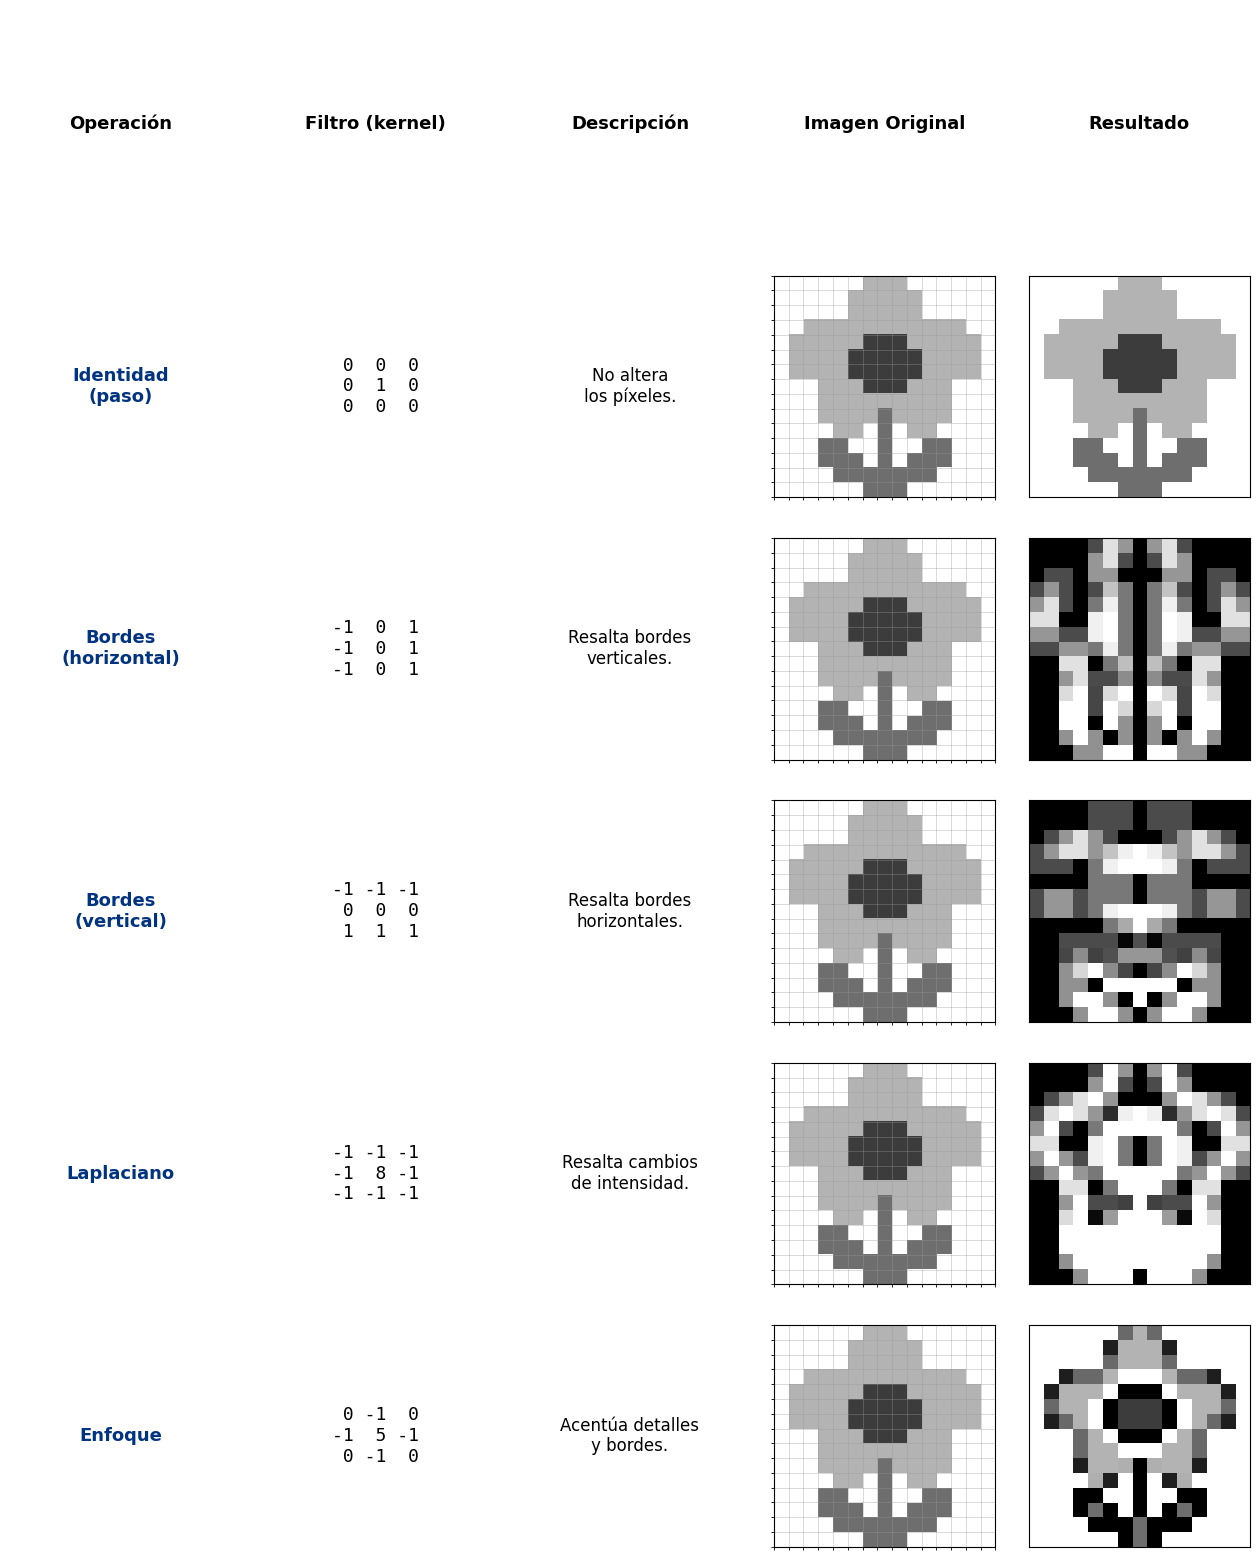
\includegraphics[keepaspectratio]{images/paste-4.png}}

}

\caption{Los distintos filtros convolucionales permiten detectar
características específicas en la imagen de entrada. En la imagen se
muestran ejemplos representativos del efecto de diferentes kernels sobre
una misma imagen.}

\end{figure}%

\section{Observación estructural}\label{observaciuxf3n-estructural}

Es importante notar que el número de filtros \(F\) determina la
capacidad de representación de la capa. Un mayor número de filtros
permite capturar una mayor variedad de patrones, pero también incrementa
el número de parámetros y el costo computacional.

En capas profundas, los filtros tienden a representar características de
mayor nivel semántico, construidas a partir de combinaciones de patrones
detectados en capas anteriores.

\bookmarksetup{startatroot}

\chapter{Stride y Padding}\label{stride-y-padding}

\section{Stride}\label{stride}

El \emph{stride} \(s\) controla el desplazamiento del kernel durante la
operación de convolución. Es decir, determina cuántas posiciones se
desplaza el kernel en cada paso.\\

Las dimensiones de salida están dadas por:

\begin{equation}\phantomsection\label{eq-output-dims}{
H' = \left\lfloor \frac{H - k_h + 2p}{s} \right\rfloor + 1, \quad
W' = \left\lfloor \frac{W - k_w + 2p}{s} \right\rfloor + 1
}\end{equation}

donde:

\begin{itemize}
\tightlist
\item
  \(H, W\) son las dimensiones de la entrada,
\item
  \(k_h, k_w\) son las dimensiones del kernel,
\item
  \(p\) es el padding,
\item
  \(s\) es el stride.
\end{itemize}

Un valor mayor de \(s\) produce una reducción en la resolución espacial
de la salida.

\section{Padding}\label{padding}

El \emph{padding} es una operación que consiste en añadir valores
(generalmente ceros) alrededor de la entrada antes de aplicar la
convolución. Esto se hace para controlar el tamaño de la salida y
preservar información en los bordes.

\[
X_{\text{pad}} \in \mathbb{R}^{(H+2p)\times(W+2p)\times C}
\]

El padding puede interpretarse como una extensión de la función de
entrada \(X\) fuera de su dominio original. Formalmente, se define la
extensión \(\tilde{X}\) como:

\[
\tilde{X}(i,j) =
\begin{cases}
X(i,j), & \text{si } (i,j) \text{ pertenece al dominio original}, \\
0, & \text{en otro caso}
\end{cases}
\]

Esta extensión corresponde a una extensión por cero del dominio de la
función.

En una capa convolucional, el padding se aplica antes de la convolución.
Por lo tanto, la operación completa de una capa convolucional con
padding se puede expresar como:

\[
Y = \sigma\big( (\text{pad}(X)) \star K + b \big)
\]

donde:

\begin{itemize}
\tightlist
\item
  \(X\) es el tensor de entrada,
\item
  \(\text{pad}(X)\) es la entrada extendida mediante padding,
\item
  \(\star\) denota la operación de correlación cruzada,
\item
  \(K\) es el kernel o filtro,
\item
  \(b\) es el sesgo,
\item
  \(\sigma\) es la función de activación.
\end{itemize}

\section{Ejemplo ilustrativo}\label{ejemplo-ilustrativo}

Para ilustrar el efecto del padding sobre las dimensiones de salida, se
presenta el siguiente ejemplo:

\begin{figure}

\centering{

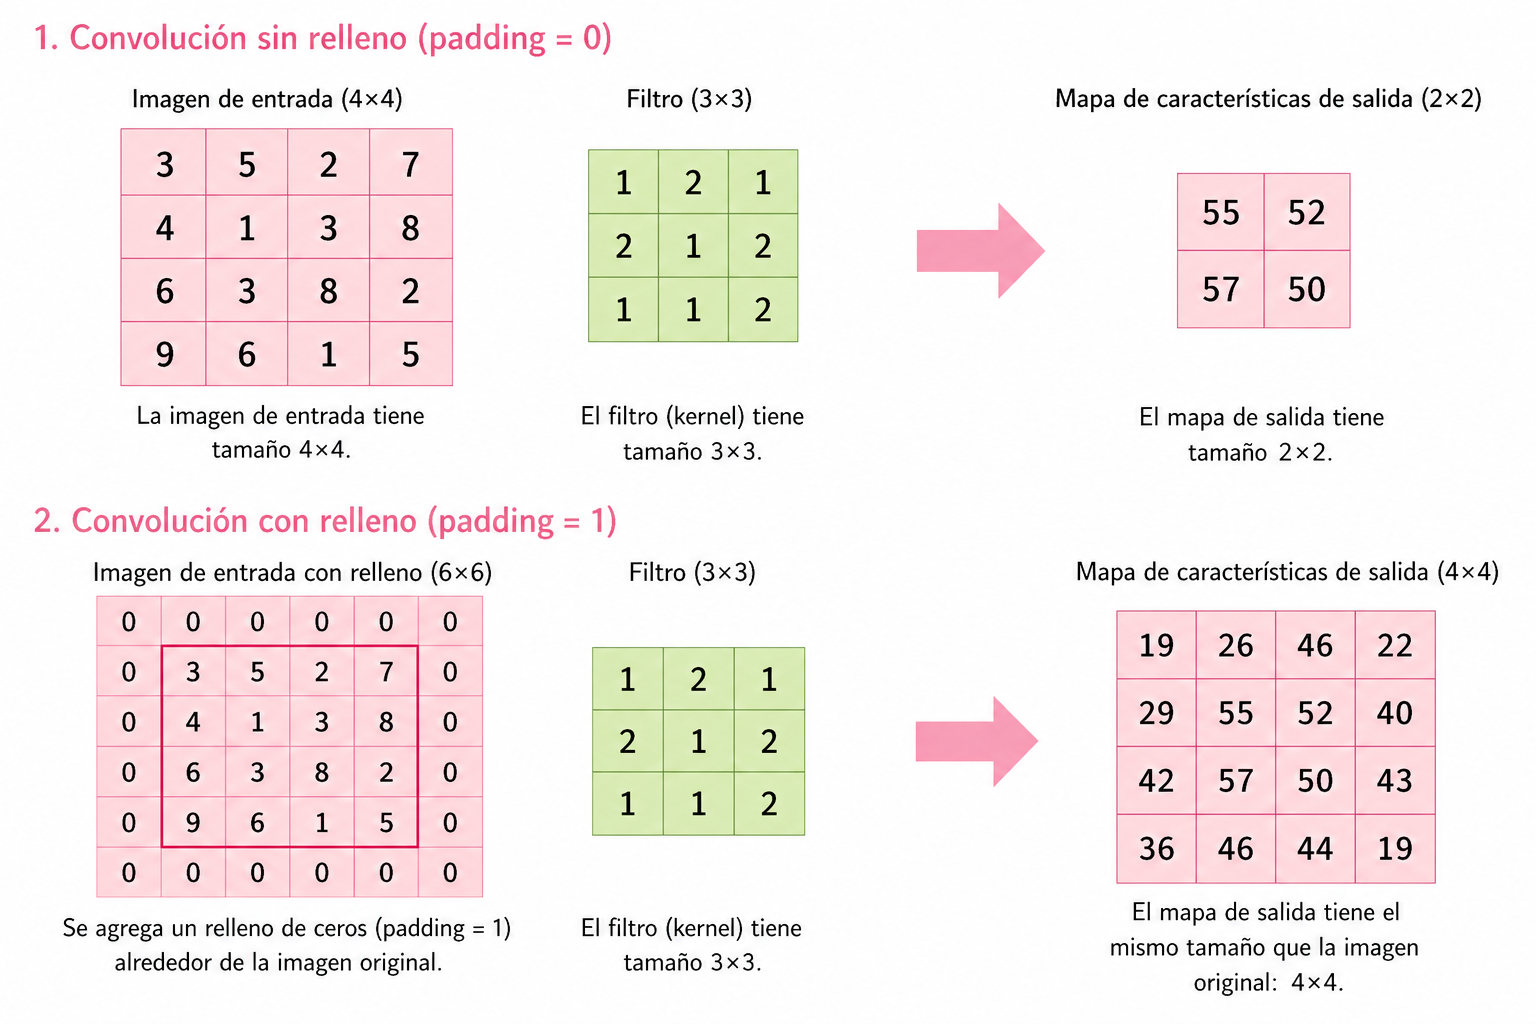
\includegraphics[width=0.8\linewidth,height=\textheight,keepaspectratio]{Imagenes_tesis/img_kernel_mapa.png}

}

\caption{\label{fig-padding}Ejemplo de convolución con y sin padding. La
incorporación de padding permite controlar el tamaño de la salida. En
particular, cuando se utiliza padding adecuado, es posible preservar las
dimensiones espaciales de la imagen original tras la aplicación de la
convolución. El color rosa identifica la imagen de entrada y la salida
de la convolución, mientras que el verde representa el filtro empleado.
En el caso del ejemplo con padding, las celdas correspondientes al
relleno se distinguen al estar por fuera del cuadro rojo, para resaltar
que no forman parte de la imagen original.}

\end{figure}%

\section{Función de activación}\label{funciuxf3n-de-activaciuxf3n}

Una función de activación es una aplicación no lineal que se introduce
después de una transformación afín, con el objetivo de dotar al modelo
de la capacidad de aproximar funciones no lineales.

\subsection{Definición}\label{definiciuxf3n}

Sea \(x \in \mathbb{R}^n\) un vector de entrada, \(w \in \mathbb{R}^n\)
un vector de pesos y \(b \in \mathbb{R}\) un sesgo. Se define la
preactivación como:

\begin{equation}\phantomsection\label{eq-preactivacion}{
z = w^T x + b
}\end{equation}

La salida de la neurona está dada por:

\begin{equation}\phantomsection\label{eq-activacion}{
y = \sigma(z)
}\end{equation}

donde \(\sigma : \mathbb{R} \to \mathbb{R}\) es la función de
activación.

\subsection{No linealidad}\label{no-linealidad}

Considérese una red neuronal profunda compuesta únicamente por
transformaciones afines. En tal caso, la composición de dichas
transformaciones satisface:

\[
f(x) = W_L W_{L-1} \cdots W_1 x + b'
\]

lo cual sigue siendo una transformación afín. Por consiguiente, sin la
introducción de funciones de activación no lineales, la red carece de
capacidad expresiva para modelar relaciones no lineales.

En una red neuronal convolucional (CNN), la salida de una capa se
expresa como:

\begin{equation}\phantomsection\label{eq-cnn-activacion}{
Y = \sigma\big( X \star K + b \big)
}\end{equation}

donde:

\begin{itemize}
\tightlist
\item
  \(X\) es el tensor de entrada\\
\item
  \(\star\) denota la operación de correlación cruzada\\
\item
  \(K\) es el conjunto de filtros (kernels)\\
\item
  \(b\) es el sesgo\\
\item
  \(\sigma\) se aplica elemento a elemento
\end{itemize}

\subsection{Ejemplos de funciones de
activación}\label{ejemplos-de-funciones-de-activaciuxf3n}

Algunas de las funciones de activación más utilizadas son las
siguientes: \begin{center}
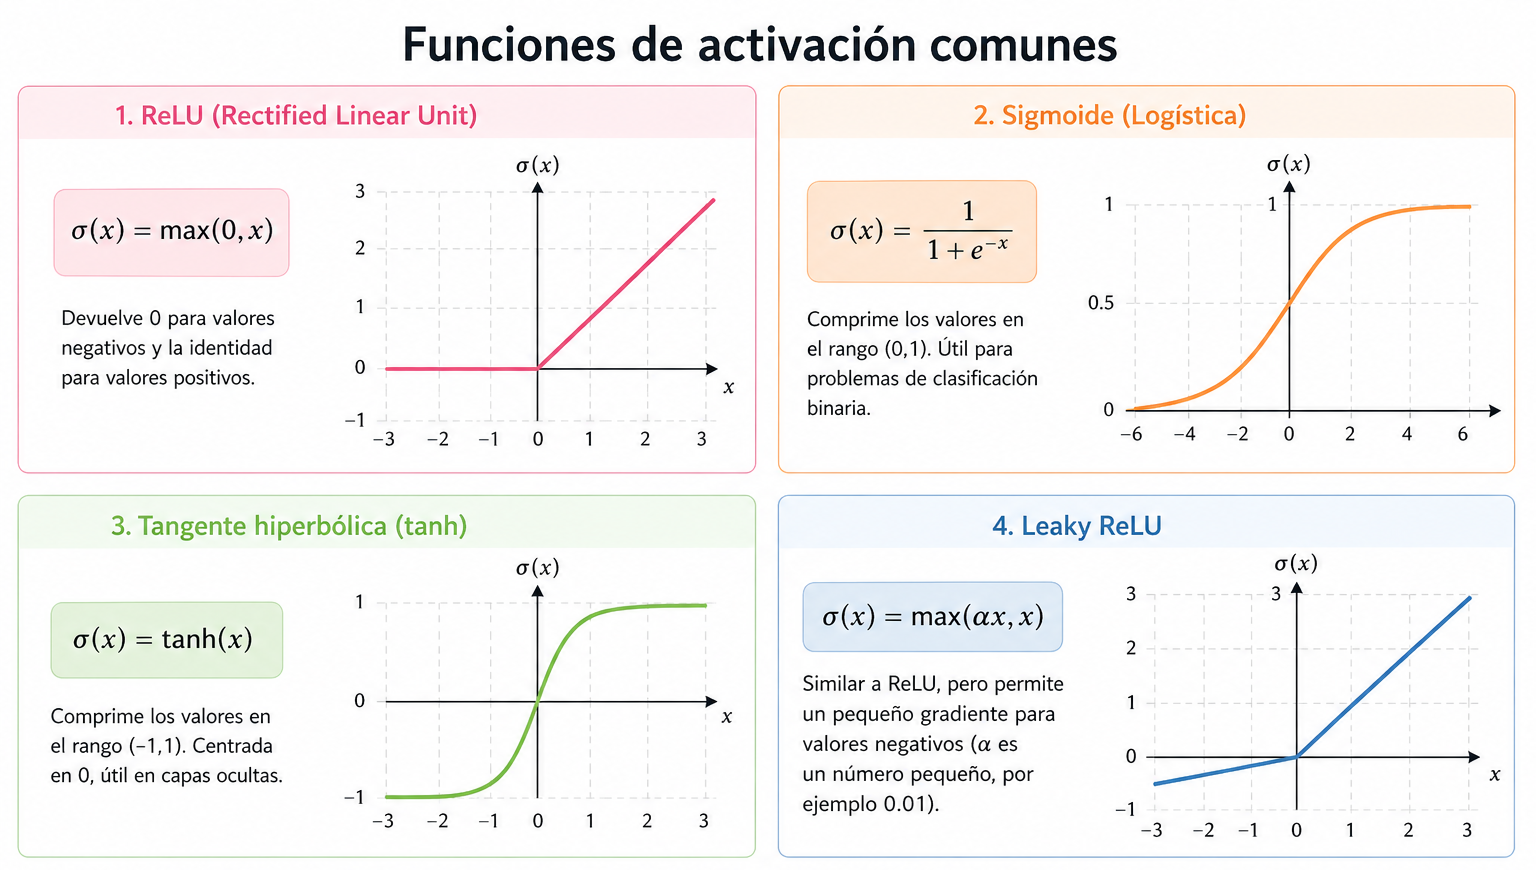
\includegraphics[width=0.82\linewidth,height=\textheight,keepaspectratio]{Imagenes_tesis/img_funciones_activacion.png}
\end{center}

\subsubsection{ReLU (Rectified Linear
Unit)}\label{relu-rectified-linear-unit}

\begin{equation}\phantomsection\label{eq-relu}{
\sigma(x) = \max(0, x)
}\end{equation}

\subsubsection{Sigmoide}\label{sigmoide}

\begin{equation}\phantomsection\label{eq-sigmoide}{
\sigma(x) = \frac{1}{1 + e^{-x}}
}\end{equation}

\subsubsection{Tangente hiperbólica}\label{tangente-hiperbuxf3lica}

\begin{equation}\phantomsection\label{eq-tanh}{
\sigma(x) = \tanh(x)
}\end{equation}

\subsection{Propiedades fundamentales}\label{propiedades-fundamentales}

Las funciones de activación empleadas en redes neuronales satisfacen
típicamente:

\begin{itemize}
\tightlist
\item
  No linealidad, necesaria para incrementar la capacidad de
  representación del modelo\\
\item
  Aplicación puntual (element-wise), preservando la estructura espacial
  en CNN\\
\item
  Diferenciabilidad (al menos casi en todas partes), requisito esencial
  para métodos de optimización basados en gradiente
\end{itemize}

\subsection{Formulación funcional}\label{formulaciuxf3n-funcional}

Desde una perspectiva funcional, una red neuronal profunda puede
interpretarse como la composición de aplicaciones de la forma:

\begin{equation}\phantomsection\label{eq-deep-functional}{
f_\theta = \sigma_L \circ T_L \circ \cdots \circ \sigma_1 \circ T_1
}\end{equation}

donde cada transformación afín está dada por:

\[
T_i(x) = W_i x + b_i
\]

\section{Pooling}\label{pooling}

El \emph{pooling} es una operación que reduce la dimensión espacial de
la representación, conservando las características más relevantes. Esta
operación se aplica de manera independiente en cada canal del tensor de
entrada.

Sea:

\[
X \in \mathbb{R}^{H \times W \times C}
\]

la entrada de la capa. El pooling produce una salida:

\[
Y \in \mathbb{R}^{H' \times W' \times C}
\]

donde las dimensiones \(H'\) y \(W'\) son menores que \(H\) y \(W\).

\subsection{Max Pooling}\label{max-pooling}

El \emph{max pooling} es la forma más común de pooling. Para cada región
local \(X_{(i,j)}\), se define:

\begin{equation}\phantomsection\label{eq-maxpool}{
Y(i,j,c) = \max_{(u,v) \in \mathcal{R}} X(i+u, j+v, c)
}\end{equation}

donde \(\mathcal{R}\) representa la ventana de pooling (por ejemplo, de
tamaño \(2 \times 2\)).

\subsection{Average Pooling}\label{average-pooling}

Otra variante es el \emph{average pooling}, definido como:

\begin{equation}\phantomsection\label{eq-avgpool}{
Y(i,j,c) = \frac{1}{|\mathcal{R}|} \sum_{(u,v) \in \mathcal{R}} X(i+u, j+v, c)
}\end{equation} El pooling sirve para reducir las dimensiones espaciales
(ancho y alto) de un tensor, asegurando que se conserve la información
más relevante. Aplicar esta técnica brinda grandes beneficios a los
modelos: disminuye significativamente el costo computacional, introduce
invariancia a pequeñas traslaciones en la imagen y ayuda a prevenir el
sobreajuste. Además, es importante destacar que esta reducción se aplica
de manera independiente a cada canal de profundidad del tensor

\begin{figure}[H]

{\centering \pandocbounded{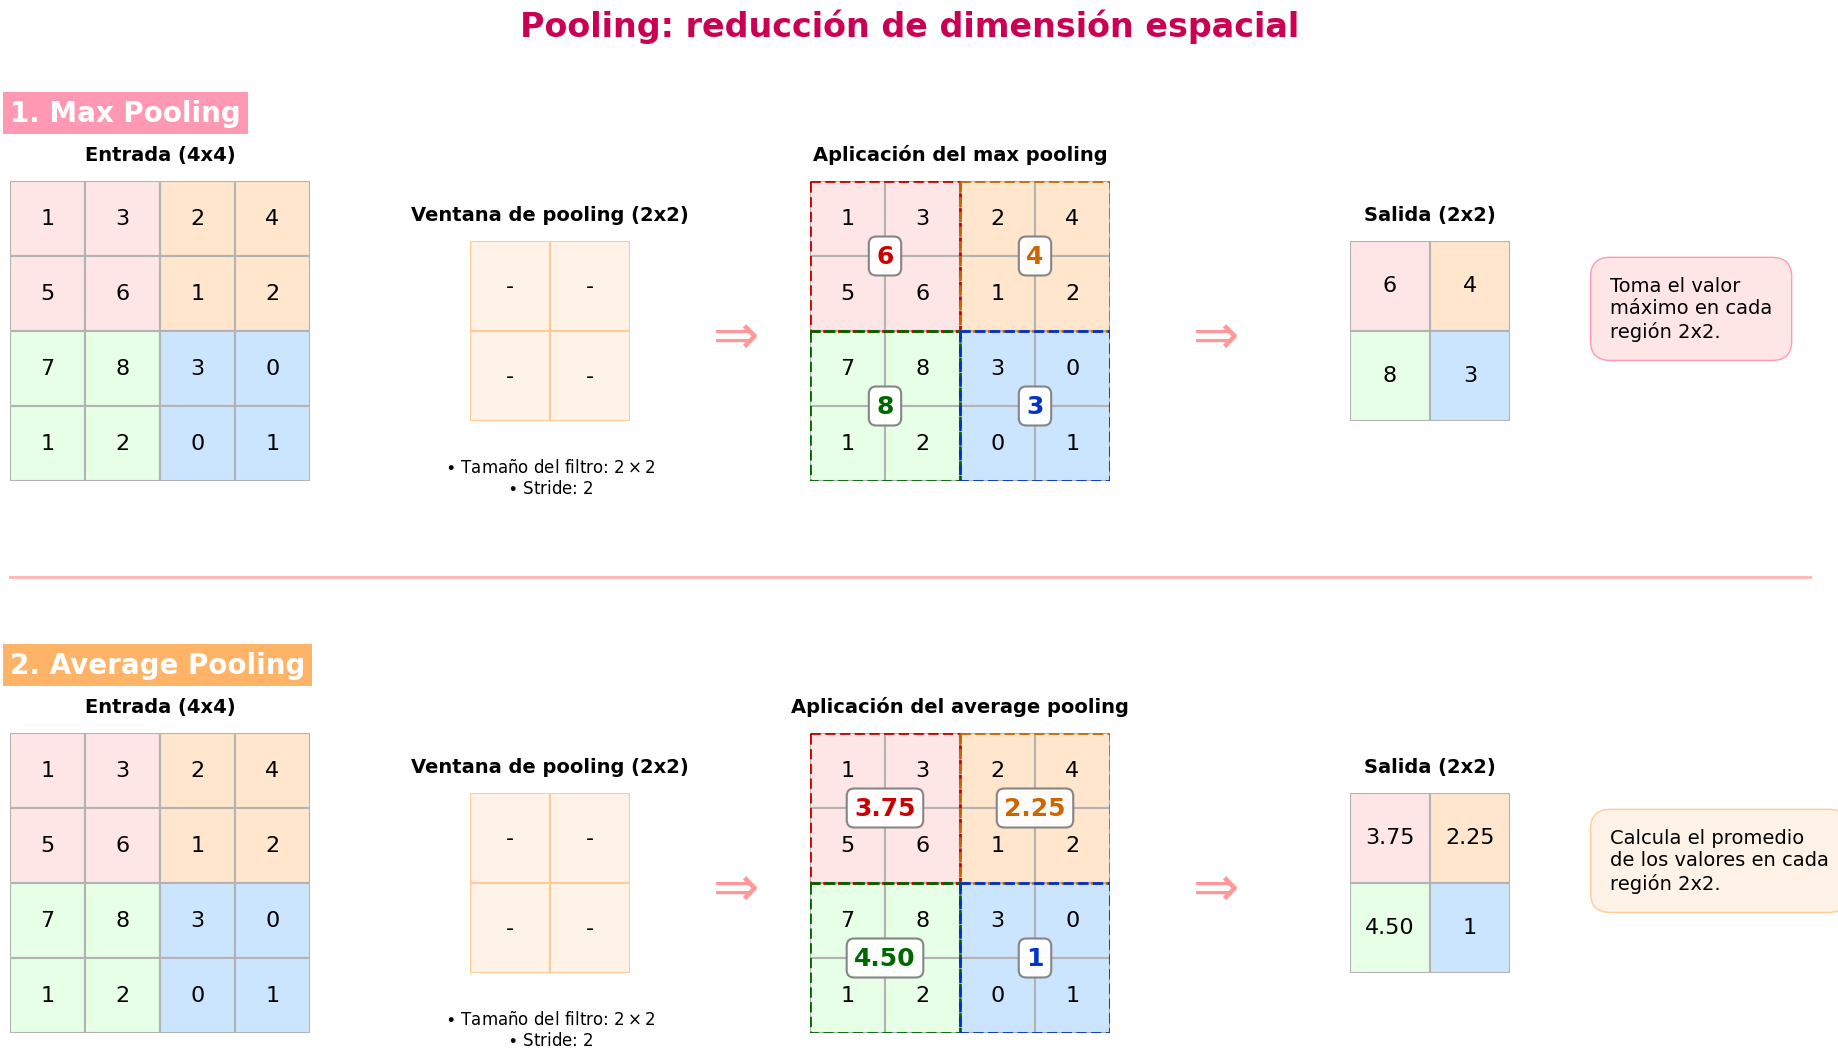
\includegraphics[keepaspectratio]{images/paste-3.png}}

}

\caption{En la parte superior de la figura se ilustra el funcionamiento
del Max Pooling utilizando una ventana de tamaño 2×2 y un stride de 2.
La imagen de entrada se divide en cuatro regiones no superpuestas,
identificadas mediante diferentes colores. Para cada región, el operador
selecciona únicamente el valor máximo: en la región superior izquierda
se obtiene 6, en la superior derecha 4, en la inferior izquierda 8 y en
la inferior derecha 3. Estos valores conforman el mapa de salida de
tamaño 2×2, preservando las características más destacadas de cada zona
mientras se reduce la dimensionalidad espacial. De manera similar, en la
parte inferior de la figura se muestra el proceso de Average Pooling con
la misma ventana 2×2 y el mismo stride. En lugar de conservar el valor
máximo, se calcula el promedio de los elementos contenidos en cada
región. Así, las cuatro ventanas generan los valores 3.75, 2.25, 4.50 y
1, que constituyen la salida reducida. Este método produce una
representación más suavizada de la información, manteniendo la tendencia
general de los datos presentes en cada región de la imagen.}

\end{figure}%

\subsection{Propiedades}\label{propiedades}

El pooling presenta las siguientes propiedades:

\begin{itemize}
\tightlist
\item
  Reduce la dimensionalidad espacial, disminuyendo el costo
  computacional\\
\item
  Introduce una cierta invariancia a traslaciones pequeñas\\
\item
  Opera de forma independiente en cada canal
\end{itemize}

\subsection{Interpretación}\label{interpretaciuxf3n}

El pooling puede interpretarse como una forma de resumen local de la
información. En el caso del max pooling, se selecciona la característica
más prominente dentro de cada región, mientras que el average pooling
produce una media de las intensidades.

En arquitecturas profundas, el pooling contribuye a la construcción de
representaciones más abstractas, al reducir progresivamente la
resolución espacial.

\section{Capas completamente
conectadas}\label{capas-completamente-conectadas}

Las capas completamente conectadas (\emph{Fully Connected}, FC)
constituyen la etapa final de una red neuronal convolucional. Su función
es combinar las características extraídas por las capas anteriores para
realizar la tarea de clasificación o regresión.

\subsection{Vectorización de la
entrada}\label{vectorizaciuxf3n-de-la-entrada}

Sea:

\[
X \in \mathbb{R}^{H \times W \times C}
\]

la salida de la última capa convolucional. Esta se transforma en un
vector mediante una operación de vectorización:

\begin{equation}\phantomsection\label{eq-vectorizacion-fc}{
x = \mathrm{vec}(X) \in \mathbb{R}^{HWC}
}\end{equation}

\subsection{Transformación afín}\label{transformaciuxf3n-afuxedn}

La capa completamente conectada aplica una transformación lineal seguida
de un sesgo:

\begin{equation}\phantomsection\label{eq-fc-lineal}{
z = Wx + b
}\end{equation}

donde:

\begin{itemize}
\tightlist
\item
  \(W \in \mathbb{R}^{k \times HWC}\) es la matriz de pesos\\
\item
  \(b \in \mathbb{R}^{k}\) es el vector de sesgos\\
\item
  \(k\) es el número de neuronas en la capa
\end{itemize}

\subsection{Aplicación de la función de
activación}\label{aplicaciuxf3n-de-la-funciuxf3n-de-activaciuxf3n}

La salida de la capa está dada por:

\begin{equation}\phantomsection\label{eq-fc-activacion}{
y = \sigma(z)
}\end{equation}

donde \(\sigma\) es una función de activación aplicada componente a
componente.

\subsection{Interpretación}\label{interpretaciuxf3n-1}

Las capas completamente conectadas pueden interpretarse como
clasificadores que operan sobre las características extraídas por la red
convolucional. En particular, cada neurona combina toda la información
disponible en la representación vectorizada.

Esto contrasta con las capas convolucionales, donde la conectividad es
local.

\subsection{Clasificación}\label{clasificaciuxf3n}

En problemas de clasificación multiclase, la última capa suele utilizar
la función \emph{softmax}, definida como:

\begin{equation}\phantomsection\label{eq-softmax}{
\text{softmax}(z_i) =
\frac{e^{z_i}}{\sum_{j=1}^{k} e^{z_j}}
}\end{equation}

Esta función transforma el vector \(z\) en una distribución de
probabilidad sobre las clases.

\subsection{Propiedades}\label{propiedades-1}

Las capas completamente conectadas presentan las siguientes
características:

\begin{itemize}
\tightlist
\item
  Conectividad global: cada neurona está conectada con todas las
  entradas\\
\item
  Alta capacidad de representación\\
\item
  Mayor número de parámetros en comparación con capas convolucionales
\end{itemize}

\subsection{Observación}\label{observaciuxf3n}

Debido al elevado número de parámetros, las capas completamente
conectadas son más propensas al sobreajuste. Por esta razón, en
arquitecturas modernas, su uso se reduce o se reemplaza parcialmente
mediante técnicas como \emph{global average pooling}.

\section{Función de pérdida}\label{funciuxf3n-de-puxe9rdida}

La función de pérdida (\emph{loss function}) cuantifica la discrepancia
entre las predicciones del modelo y los valores reales. Constituye el
criterio fundamental que guía el proceso de entrenamiento, ya que
permite evaluar la calidad de las predicciones y definir un objetivo de
optimización.

\subsection{Definición general}\label{definiciuxf3n-general}

Sea \(f_\theta(x)\) la salida del modelo para una entrada \(x\), y sea
\(y\) la etiqueta real asociada. Una función de pérdida se define como:

\[
\mathcal{L}(f_\theta(x), y)
\]

donde \(\mathcal{L} : \mathbb{R}^k \times \mathbb{R}^k \to \mathbb{R}\)
mide el error entre la predicción y el valor objetivo.

Dado un conjunto de datos \(\{(x_i, y_i)\}_{i=1}^{N}\), la función de
costo global se define como:

\begin{equation}\phantomsection\label{eq-risk}{
J(\theta) = \frac{1}{N} \sum_{i=1}^{N} \mathcal{L}(f_\theta(x_i), y_i)
}\end{equation}

\subsection{Clasificación multiclase: Entropía
cruzada}\label{clasificaciuxf3n-multiclase-entropuxeda-cruzada}

En problemas de clasificación multiclase, la función de pérdida más
utilizada es la entropía cruzada (\emph{cross-entropy}).

Sea \(p = f_\theta(x)\) la salida del modelo después de aplicar la
función \emph{softmax}, y sea \(y\) un vector one-hot que representa la
clase verdadera. La pérdida se define como:

\begin{equation}\phantomsection\label{eq-cross-entropy}{
\mathcal{L}(p, y) = - \sum_{j=1}^{k} y_j \log(p_j)
}\end{equation}

Dado que \(y\) es un vector one-hot, esta expresión se reduce a:

\[
\mathcal{L}(p, y) = -\log(p_{y})
\]

donde \(p_y\) es la probabilidad asignada a la clase correcta.

\subsection{Interpretación
probabilística}\label{interpretaciuxf3n-probabiluxedstica}

La entropía cruzada puede interpretarse como una medida de divergencia
entre la distribución verdadera \(y\) y la distribución predicha \(p\).
Minimizar esta función equivale a maximizar la probabilidad de observar
los datos bajo el modelo.

Desde un punto de vista estadístico, este enfoque corresponde al método
de máxima verosimilitud.

\subsection{Caso de regresión: Error cuadrático
medio}\label{caso-de-regresiuxf3n-error-cuadruxe1tico-medio}

En problemas de regresión, una función de pérdida común es el error
cuadrático medio (\emph{Mean Squared Error}, MSE), definido como:

\begin{equation}\phantomsection\label{eq-mse}{
\mathcal{L}(f_\theta(x), y) = \| f_\theta(x) - y \|^2
}\end{equation}

Esta función penaliza de manera más severa los errores grandes, lo que
favorece ajustes más precisos.

\subsection{Relación con el
entrenamiento}\label{relaciuxf3n-con-el-entrenamiento}

El objetivo del entrenamiento consiste en encontrar los parámetros
\(\theta\) que minimizan la función de costo global:

\begin{equation}\phantomsection\label{eq-opt}{
\theta^* = \arg\min_{\theta} J(\theta)
}\end{equation}

Este problema se resuelve típicamente mediante métodos de optimización
iterativos, como el descenso por gradiente y sus variantes.

\section{Entrenamiento}\label{entrenamiento}

El entrenamiento de una red neuronal convolucional consiste en ajustar
los parámetros \(\theta\) del modelo con el objetivo de minimizar la
función de pérdida definida previamente.

Dado un conjunto de datos \(\{(x_i, y_i)\}_{i=1}^{N}\), el problema de
entrenamiento puede formularse como:

\begin{equation}\phantomsection\label{eq-entrenamiento}{
\min_{\theta} J(\theta) = \frac{1}{N} \sum_{i=1}^{N} \mathcal{L}(f_\theta(x_i), y_i)
}\end{equation}

\subsection{Método del descenso del
gradiente}\label{muxe9todo-del-descenso-del-gradiente}

Considérese el problema de optimización irrestricta

\[
\min_{x \in \mathbb{R}^n} f(x),
\]

donde \(f:\mathbb{R}^n \to \mathbb{R}\) es una función diferenciable. El
objetivo consiste en construir un procedimiento iterativo que permita
aproximarse a un punto minimizante de \(f\). Entre los métodos más
importantes para resolver este tipo de problemas se encuentra el método
del descenso del gradiente, también conocido como \emph{gradient
descent} o método del máximo descenso.

La idea fundamental del método proviene de la interpretación geométrica
del gradiente. Para una función diferenciable \(f\), el vector gradiente

\[
\nabla f(x)
=
\begin{pmatrix}
\dfrac{\partial f}{\partial x_1}(x) \\
\dfrac{\partial f}{\partial x_2}(x) \\
\vdots \\
\dfrac{\partial f}{\partial x_n}(x)
\end{pmatrix}
\]

indica la dirección de máximo crecimiento local de la función en el
punto \(x\). En consecuencia, el vector opuesto

\[
-\nabla f(x)
\]

corresponde a la dirección de máximo decrecimiento local. El método del
descenso del gradiente aprovecha precisamente esta propiedad para
generar una sucesión de iterados que produzca una disminución progresiva
del valor de la función objetivo.

Partiendo de un punto inicial \(x_0 \in \mathbb{R}^n\), el método
construye una sucesión \(\{x_k\}\) definida mediante la iteración

\[
x_{k+1}
=
x_k - \alpha_k \nabla f(x_k),
\]

donde \(\alpha_k > 0\) representa el tamaño de paso asociado a la
iteración \(k\). La elección de este parámetro resulta fundamental para
el desempeño del algoritmo, pues determina la magnitud del
desplazamiento realizado en la dirección de descenso.

La justificación matemática del método se obtiene a partir de la noción
de dirección de descenso. Sea

\[
d_k = -\nabla f(x_k).
\]

Entonces,

\[
\nabla f(x_k)^T d_k
=
\nabla f(x_k)^T(-\nabla f(x_k))
=
-\|\nabla f(x_k)\|^2.
\]

Si \(\nabla f(x_k)\neq 0\), se tiene que

\[
\|\nabla f(x_k)\|^2 > 0,
\]

y por tanto

\[
\nabla f(x_k)^T d_k < 0.
\]

Esto demuestra que \(d_k\) constituye una dirección estricta de descenso
para la función \(f\). En otras palabras, existe un valor
suficientemente pequeño de \(\alpha > 0\) tal que

\[
f(x_k+\alpha d_k) < f(x_k).
\]

Esta propiedad puede analizarse con mayor detalle mediante el desarrollo
de Taylor de primer orden. Para \(\alpha\) pequeño se tiene

\[
f(x_k+\alpha d_k)
=
f(x_k)
+
\alpha \nabla f(x_k)^T d_k
+
o(\alpha).
\]

Sustituyendo \(d_k=-\nabla f(x_k)\), resulta

\[
f(x_k-\alpha \nabla f(x_k))
=
f(x_k)
-
\alpha \|\nabla f(x_k)\|^2
+
o(\alpha).
\]

Debido a que el término dominante es negativo, el valor de la función
disminuye localmente para valores suficientemente pequeños de
\(\alpha\). Esta observación constituye la base teórica del algoritmo.

La selección del tamaño de paso \(\alpha_k\) es uno de los aspectos
centrales del método. Una posibilidad consiste en utilizar un paso
constante,

\[
\alpha_k = \alpha,
\]

lo cual simplifica considerablemente la implementación. Sin embargo, si
el valor de \(\alpha\) es demasiado grande, la sucesión puede divergir o
presentar oscilaciones; por el contrario, si \(\alpha\) es demasiado
pequeño, la convergencia puede resultar excesivamente lenta.

Otra estrategia consiste en determinar el tamaño de paso mediante una
búsqueda lineal exacta. En este caso, \(\alpha_k\) se obtiene
resolviendo el problema unidimensional

\[
\alpha_k
=
\arg\min_{\alpha>0}
f(x_k-\alpha \nabla f(x_k)).
\]

De esta manera, en cada iteración se minimiza exactamente la función
sobre la recta definida por la dirección de descenso. Aunque este
enfoque posee una sólida justificación teórica, en problemas de gran
dimensión suele resultar costoso desde el punto de vista computacional.
Por esta razón, frecuentemente se emplean búsquedas lineales inexactas
basadas en criterios como las condiciones de Armijo o de Wolfe, las
cuales garantizan una reducción suficiente de la función objetivo sin
resolver completamente el subproblema unidimensional.

El criterio de terminación más habitual se basa en la norma del
gradiente. Dado que un punto minimizante diferenciable debe satisfacer
la condición necesaria de primer orden

\[
\nabla f(x^\ast)=0,
\]

el algoritmo suele detenerse cuando

\[
\|\nabla f(x_k)\| < \varepsilon,
\]

para cierta tolerancia \(\varepsilon > 0\).

Las propiedades de convergencia del método dependen de las
características de la función objetivo. Si \(f\) es convexa y su
gradiente es Lipschitz continuo, entonces la sucesión generada por el
método converge hacia un mínimo global. Más aún, si \(f\) es fuertemente
convexa, es decir, si existe \(\mu>0\) tal que

\[
f(y)
\geq
f(x)
+
\nabla f(x)^T(y-x)
+
\frac{\mu}{2}\|y-x\|^2,
\]

entonces el método presenta convergencia lineal para elecciones
apropiadas del tamaño de paso.

Para ilustrar el procedimiento, considérese la función cuadrática

\[
f(x,y)=x^2+y^2.
\]

Su gradiente está dado por

\[
\nabla f(x,y)
=
\begin{pmatrix}
2x\\
2y
\end{pmatrix}.
\]

En consecuencia, la iteración del descenso del gradiente toma la forma

\[
\begin{pmatrix}
x_{k+1}\\
y_{k+1}
\end{pmatrix}
=
\begin{pmatrix}
x_k\\
y_k
\end{pmatrix}
-
\alpha
\begin{pmatrix}
2x_k\\
2y_k
\end{pmatrix},
\]

lo cual equivale a

\[
x_{k+1}=(1-2\alpha)x_k,
\qquad
y_{k+1}=(1-2\alpha)y_k.
\]

La convergencia hacia el origen ocurre siempre que

\[
0<\alpha<1.
\]

A pesar de su simplicidad y relevancia teórica, el método del descenso
del gradiente posee ciertas limitaciones. En funciones mal
condicionadas, la trayectoria de los iterados puede presentar
oscilaciones pronunciadas y convergencia lenta, especialmente en
regiones con geometría alargada o estrecha. Asimismo, en problemas no
convexos el método puede converger hacia mínimos locales o puntos silla.

No obstante, el descenso del gradiente constituye la base conceptual de
numerosos algoritmos modernos de optimización y aprendizaje automático,
entre ellos el descenso estocástico del gradiente, los métodos con
momentum, Nesterov, AdaGrad, RMSProp y Adam. Además, mantiene una
estrecha relación con métodos de segundo orden como Newton y los
algoritmos quasi-Newton.

Finalmente, el método admite una interpretación continua particularmente
elegante. La iteración discreta puede verse como una aproximación
numérica de la ecuación diferencial

\[
\frac{dx(t)}{dt}
=
-\nabla f(x(t)),
\]

conocida como flujo de gradiente (\emph{gradient flow}). Esta ecuación
describe una dinámica continua en la cual el sistema evoluciona
siguiendo la dirección de máximo decrecimiento de la función energía
\(f\).

\subsection{Regla de la cadena y
retropropagación}\label{regla-de-la-cadena-y-retropropagaciuxf3n}

El cálculo del gradiente en redes neuronales profundas se realiza
mediante el algoritmo de retropropagación (\emph{backpropagation}), el
cual se basa en la aplicación sistemática de la regla de la cadena.

Sea una red expresada como:

\[
f_\theta = f^{(L)} \circ \cdots \circ f^{(1)}
\]

el gradiente de la pérdida respecto a los parámetros de una capa \(l\)
se obtiene propagando el error desde la salida hacia las capas
anteriores.

Este procedimiento permite calcular eficientemente:

\[
\nabla_{\theta^{(l)}} J(\theta)
\]

para cada capa \(l\) de la red.

\section{Regularización}\label{regularizaciuxf3n}

En el entrenamiento de redes neuronales, es común que el modelo se
ajuste excesivamente a los datos de entrenamiento, fenómeno conocido
como \emph{sobreajuste} (\emph{overfitting}). En este caso, el modelo
presenta un buen desempeño en los datos de entrenamiento, pero
generaliza pobremente a datos no vistos.

La regularización consiste en un conjunto de técnicas diseñadas para
mejorar la capacidad de generalización del modelo.

\subsection{Sobreajuste}\label{sobreajuste}

El sobreajuste ocurre cuando el modelo aprende no solo las
características relevantes del problema, sino también el ruido presente
en los datos. Esto suele suceder cuando el modelo tiene una alta
capacidad de representación en relación con la cantidad de datos
disponibles.

\subsection{Penalización de parámetros (Weight
Decay)}\label{penalizaciuxf3n-de-paruxe1metros-weight-decay}

Una estrategia común consiste en añadir un término de penalización a la
función de costo:

\begin{equation}\phantomsection\label{eq-regularizacion-l2}{
J(\theta) = \frac{1}{N} \sum_{i=1}^{N} \mathcal{L}(f_\theta(x_i), y_i) + \lambda \|\theta\|^2
}\end{equation}

donde:

\begin{itemize}
\tightlist
\item
  \(\lambda > 0\) es el parámetro de regularización\\
\item
  \(\|\theta\|^2\) es la norma cuadrática de los parámetros
\end{itemize}

Este término penaliza valores grandes de los parámetros, favoreciendo
modelos más simples.

\subsection{Dropout}\label{dropout}

El \emph{dropout} es una técnica de regularización utilizada en redes
neuronales profundas cuyo objetivo principal es reducir el sobreajuste y
mejorar la capacidad de generalización del modelo. La idea esencial
consiste en introducir aleatoriedad durante el entrenamiento mediante la
desactivación temporal de neuronas. Como consecuencia, en cada iteración
se entrena efectivamente una subred distinta de la arquitectura
original.

Consideremos una capa neuronal cuya entrada es un vector

\[
x \in \mathbb{R}^{H\times W\times C},
\]

con matriz de pesos

\[
W \in \mathbb{R}^{m\times d}
\]

donde hay \(m\) neuronas. Y vector de sesgos

\[
b\in\mathbb{R}^m.
\]

La salida usual de la capa está dada por

\[
h=\phi(Wx+b).
\]

El mecanismo de dropout introduce un vector aleatorio

\[
r=(r_1,\dots,r_m),
\]

cuyas componentes son independientes y satisfacen

\[
r_i\sim\operatorname{Bernoulli}(p).
\] Aquí, el parámetro \(p\in(0,1]\) representa la probabilidad de
conservar activa una neurona durante el entrenamiento. En consecuencia,
cada neurona tiene probabilidad \(1-p\) de ser anulada temporalmente.

La nueva activación de la capa se define entonces por

\[
\tilde h=r\odot h,
\]

donde \(\odot\) denota el producto componente a componente. De esta
forma, si \(r_i=0\), la activación correspondiente desaparece
completamente en esa iteración; si \(r_i=1\), la neurona permanece
activa.

En implementaciones modernas suele utilizarse la variante denominada
\emph{inverted dropout}, en la cual las activaciones se reescalan
durante el entrenamiento:

\[
\tilde h=\frac{r}{p}\odot h.
\]

La razón matemática de este reescalamiento es preservar el valor
esperado de las activaciones. En efecto, puesto que

\[
\mathbb{E}[r_i]=p,
\]

se obtiene

\[
\mathbb{E}\left[\frac{r_i}{p}h_i\right]
=
\frac{1}{p}\mathbb{E}[r_i]h_i
=
h_i.
\]

Por tanto, el valor esperado de las activaciones permanece invariante:

\[
\mathbb{E}[\tilde h]=h.
\]

Gracias a esta propiedad, durante la etapa de inferencia no es necesario
realizar ajustes adicionales: simplemente se utiliza la red completa sin
eliminar neuronas.

Desde un punto de vista probabilístico, el dropout puede interpretarse
como un procedimiento que entrena simultáneamente un gran conjunto de
subredes. Si una red posee \(n\) neuronas susceptibles de ser
desactivadas, entonces existen potencialmente

\[
2^n
\]

subredes distintas. El entrenamiento explícito de todas ellas sería
computacionalmente inviable; sin embargo, el dropout proporciona una
aproximación eficiente a un promedio implícito sobre dicho ensamble de
modelos.

La relevancia de esta idea se encuentra en que las redes neuronales
poseen una enorme capacidad de representación y, por ello, pueden
memorizar patrones específicos del conjunto de entrenamiento. Cuando
ciertas neuronas dependen excesivamente de otras, aparecen fenómenos de
\emph{co-adaptación}. El dropout rompe estas dependencias debido a que
cualquier neurona puede desaparecer aleatoriamente durante el
entrenamiento. Como consecuencia, cada unidad debe aprender
representaciones más independientes y robustas.

Formalmente, el entrenamiento ya no minimiza una función de pérdida
determinista, sino una pérdida esperada respecto de la aleatoriedad
introducida por las máscaras de dropout. Si \(m\) representa una
realización particular de la máscara aleatoria y \(\theta\) denota el
conjunto de parámetros de la red, entonces el problema de optimización
puede escribirse como

\[
\min_\theta
\;
\mathbb{E}_m
\left[
\mathcal{L}(f(x;m,\theta),y)
\right].
\]

Aquí, \(f(x;m,\theta)\) representa la subred inducida por la máscara
\(m\). Así, cada actualización del descenso del gradiente se realiza
sobre una arquitectura ligeramente distinta.

Si el descenso del gradiente estándar actualiza parámetros mediante

\[
\theta_{t+1}
=
\theta_t
-
\eta\nabla_\theta\mathcal{L}(\theta_t),
\]

entonces bajo dropout la actualización toma la forma

\[
\theta_{t+1}
=
\theta_t
-
\eta
\nabla_\theta
\mathcal{L}(f(x;m_t,\theta_t),y),
\]

donde \(m_t\) es una máscara aleatoria distinta en cada iteración. Este
ruido adicional actúa como un mecanismo regularizador que dificulta el
ajuste excesivamente preciso a los datos de entrenamiento.

En ciertos modelos simples, particularmente lineales, puede demostrarse
que el dropout induce aproximadamente un efecto regularizador semejante
a una penalización cuadrática sobre los pesos. En este sentido, su
comportamiento se relaciona parcialmente con métodos de regularización
tipo \(L^2\), aunque el mecanismo subyacente es distinto, ya que aquí la
regularización surge a partir de una perturbación aleatoria
multiplicativa.

Desde una perspectiva geométrica, el dropout favorece representaciones
distribuidas y estables frente a perturbaciones. Una neurona no puede
depender de la presencia permanente de otras unidades, de modo que la
información relevante termina siendo compartida entre múltiples
componentes de la red. Esto produce modelos menos frágiles y con mejor
capacidad de generalización.

Aunque arquitecturas modernas incorporan otros mecanismos de
regularización, como \emph{Batch Normalization} y conexiones residuales,
el dropout continúa siendo una herramienta fundamental, especialmente en
redes densas tradicionales y en problemas donde la cantidad de datos
disponibles es limitada.

\section{Optimización}\label{optimizaciuxf3n}

El proceso de entrenamiento de una red neuronal implica la resolución de
un problema de optimización en alta dimensión. En la práctica, este
problema se aborda mediante métodos iterativos basados en gradiente.

\subsection{Descenso por gradiente estocástico
(SGD)}\label{descenso-por-gradiente-estocuxe1stico-sgd}

En lugar de utilizar todo el conjunto de datos en cada iteración, el
\emph{Stochastic Gradient Descent} (SGD) emplea subconjuntos
(mini-batches):

\[
\theta \leftarrow \theta - \eta \nabla_{\theta} \mathcal{L}(f_\theta(x_i), y_i)
\]

Este enfoque reduce el costo computacional y permite actualizaciones más
frecuentes.

\subsection{Mini-batch gradient
descent}\label{mini-batch-gradient-descent}

Una generalización del SGD consiste en utilizar lotes de tamaño
intermedio:

\begin{equation}\phantomsection\label{eq-minibatch}{
\theta \leftarrow \theta - \eta \frac{1}{B} \sum_{i=1}^{B} \nabla_{\theta} \mathcal{L}(f_\theta(x_i), y_i)
}\end{equation}

donde \(B\) es el tamaño del lote.

\subsection{Métodos adaptativos}\label{muxe9todos-adaptativos}

Existen métodos de optimización que ajustan automáticamente la tasa de
aprendizaje para cada parámetro. Uno de los más utilizados es
\emph{Adam}.

El algoritmo Adam combina ideas de momento y escalamiento adaptativo del
gradiente. De manera simplificada, realiza actualizaciones de la forma:

\[
\theta \leftarrow \theta - \eta \frac{m_t}{\sqrt{v_t} + \epsilon}
\]

donde:

\begin{itemize}
\tightlist
\item
  \(m_t\) es el promedio exponencial de los gradientes\\
\item
  \(v_t\) es el promedio exponencial de los gradientes al cuadrado\\
\item
  \(\epsilon\) es un término de estabilidad numérica
\end{itemize}

\subsection{Tasa de aprendizaje}\label{tasa-de-aprendizaje}

La tasa de aprendizaje \(\eta\) controla la magnitud de las
actualizaciones. Su elección es crucial:

\begin{itemize}
\tightlist
\item
  valores pequeños producen convergencia lenta\\
\item
  valores grandes pueden causar inestabilidad
\end{itemize}

En la práctica, se utilizan esquemas de decaimiento de la tasa de
aprendizaje.

\bookmarksetup{startatroot}

\chapter{Fundamentos teóricos: Cadenas de Markov a Tiempo Continuo y
Modelos
Ocultos}\label{fundamentos-teuxf3ricos-cadenas-de-markov-a-tiempo-continuo-y-modelos-ocultos}

\bookmarksetup{startatroot}

\chapter{Espacio Probabilístico y Procesos Estocásticos
Subyacentes}\label{espacio-probabiluxedstico-y-procesos-estocuxe1sticos-subyacentes}

Para establecer formalmente una Cadena de Markov a Tiempo Continuo
(CTMC), es necesario partir de los axiomas fundamentales de la teoría de
la medida, para más detalle consultar el libro de @Rudin1987.

Para esto, se asumirá que el lector tiene conocimientos previos sobre
teoría de la medida como lo son las \(\sigma\)-álgebras, espacio
muestral y medida de probabilidad, entre otros.

\begin{tcolorbox}[enhanced jigsaw, leftrule=.75mm, colback=white, arc=.35mm, coltitle=black, bottomtitle=1mm, colbacktitle=quarto-callout-note-color!10!white, toprule=.15mm, title=\textcolor{quarto-callout-note-color}{\faInfo}\hspace{0.5em}{Nota \ref*{nte-espacio-filtrado}: Definición (Espacio de Probabilidad Filtrado)}, opacityback=0, left=2mm, toptitle=1mm, titlerule=0mm, rightrule=.15mm, colframe=quarto-callout-note-color-frame, bottomrule=.15mm, breakable, opacitybacktitle=0.6]

\quartocalloutnte{nte-espacio-filtrado} 

Sea \((\Omega, \mathcal{F}, \mathbb{P})\) un espacio de probabilidad,
donde \(\Omega\) es el espacio muestral, \(\mathcal{F}\) es una
\(\sigma\)-álgebra sobre \(\Omega\), y \(\mathbb{P}\) es una medida de
probabilidad. Sea \(\mathbb{F} = \{\mathcal{F}_t\}_{t \ge 0}\) una
filtración, es decir, una familia no decreciente de
sub-\(\sigma\)-álgebras de \(\mathcal{F}\) tal que
\(\mathcal{F}_s \subseteq \mathcal{F}_t \subseteq \mathcal{F}\) para
todo \(0 \le s < t\). El conjunto
\((\Omega, \mathcal{F}, \mathbb{F}, \mathbb{P})\) se denomina espacio de
probabilidad filtrado.

\end{tcolorbox}

\begin{tcolorbox}[enhanced jigsaw, leftrule=.75mm, colback=white, arc=.35mm, coltitle=black, bottomtitle=1mm, colbacktitle=quarto-callout-note-color!10!white, toprule=.15mm, title=\textcolor{quarto-callout-note-color}{\faInfo}\hspace{0.5em}{Nota \ref*{nte-espacio-estados-discreto}: Definición (Espacio de Estados Discreto)}, opacityback=0, left=2mm, toptitle=1mm, titlerule=0mm, rightrule=.15mm, colframe=quarto-callout-note-color-frame, bottomrule=.15mm, breakable, opacitybacktitle=0.6]

\quartocalloutnte{nte-espacio-estados-discreto} 

Definimos el espacio de estados \(S\) como un conjunto discreto y finito
(o numerable).

La topología en \(S\) es discreta y su \(\sigma\)-álgebra asociada es el
conjunto potencia \(\mathcal{P}(S)\).

\end{tcolorbox}

En el contexto de nuestro proyecto, \(S\) representa el conjunto de
posibles colores o intensidades de un pixel (por ejemplo, el espacio RGB
donde \(|S| = 256^3\), o una escala de grises finita).

\begin{tcolorbox}[enhanced jigsaw, leftrule=.75mm, colback=white, arc=.35mm, coltitle=black, bottomtitle=1mm, colbacktitle=quarto-callout-note-color!10!white, toprule=.15mm, title=\textcolor{quarto-callout-note-color}{\faInfo}\hspace{0.5em}{Nota \ref*{nte-proceso-estocastico}: Definición (Proceso Estocástico a Tiempo Continuo)}, opacityback=0, left=2mm, toptitle=1mm, titlerule=0mm, rightrule=.15mm, colframe=quarto-callout-note-color-frame, bottomrule=.15mm, breakable, opacitybacktitle=0.6]

\quartocalloutnte{nte-proceso-estocastico} 

Un proceso estocástico en tiempo continuo con espacio de estados
discreto \(S\) es una familia de variables aleatorias

\[
X = \{X(t) : t \in \mathbb{R}_{\ge 0}\},
\]

donde cada \(X(t): \Omega \to S\) es una función medible respecto a
\(\mathcal{F}_t\).

\end{tcolorbox}

Interpretamos \(X(t)\) como el ``color verdadero'' del pixel en el
instante (o parámetro continuo) \(t\).

\bookmarksetup{startatroot}

\chapter{Cadenas de Markov a Tiempo Continuo
(CTMC)}\label{cadenas-de-markov-a-tiempo-continuo-ctmc}

La transición del concepto general de proceso estocástico al de proceso
de Markov requiere la propiedad de amnesia (pérdida de memoria).

\begin{tcolorbox}[enhanced jigsaw, leftrule=.75mm, colback=white, arc=.35mm, coltitle=black, bottomtitle=1mm, colbacktitle=quarto-callout-note-color!10!white, toprule=.15mm, title=\textcolor{quarto-callout-note-color}{\faInfo}\hspace{0.5em}{Nota \ref*{nte-propiedad-markov}: Definición (Propiedad de Markov)}, opacityback=0, left=2mm, toptitle=1mm, titlerule=0mm, rightrule=.15mm, colframe=quarto-callout-note-color-frame, bottomrule=.15mm, breakable, opacitybacktitle=0.6]

\quartocalloutnte{nte-propiedad-markov} 

El proceso adaptado \(X = \{X(t)\}_{t \ge 0}\) es una Cadena de Markov a
Tiempo Continuo si satisface la condición de Markov relativa a la
filtración \(\mathbb{F}\): para cualquier conjunto discreto de tiempos

\[
0 \le t_1 < t_2 < \dots < t_n < t
\]

y cualquier secuencia de estados

\[
i_1, i_2, \dots, i_n, i, j \in S,
\]

se cumple que

\[
\mathbb{P}(X(t) = j \mid X(t_1) = i_1, \dots, X(t_n) = i, X(s) = i)
=
\mathbb{P}(X(t) = j \mid X(s) = i).
\]

De manera equivalente y más elegante mediante la esperanza condicional:

\[
\mathbb{P}(X(t) = j \mid \mathcal{F}_s)
=
\mathbb{P}(X(t) = j \mid X(s))
\quad
\text{c.s. (casi seguramente)}
\]

para todo \(0 \le s \le t\).

\end{tcolorbox}

\begin{tcolorbox}[enhanced jigsaw, leftrule=.75mm, colback=white, arc=.35mm, coltitle=black, bottomtitle=1mm, colbacktitle=quarto-callout-note-color!10!white, toprule=.15mm, title=\textcolor{quarto-callout-note-color}{\faInfo}\hspace{0.5em}{Nota \ref*{nte-probabilidades-transicion}: Definición (Probabilidades de Transición y Homogeneidad)}, opacityback=0, left=2mm, toptitle=1mm, titlerule=0mm, rightrule=.15mm, colframe=quarto-callout-note-color-frame, bottomrule=.15mm, breakable, opacitybacktitle=0.6]

\quartocalloutnte{nte-probabilidades-transicion} 

Definimos la probabilidad de transición del estado \(i\) al estado \(j\)
en el intervalo \([s,t]\) como

\[
p_{ij}(s,t)
=
\mathbb{P}(X(t)=j \mid X(s)=i).
\]

Se dice que la CTMC es \textbf{homogénea en el tiempo} si
\(p_{ij}(s,t)\) depende únicamente de la longitud del intervalo temporal

\[
\tau=t-s.
\]

En tal caso, denotamos la probabilidad de transición como

\[
p_{ij}(\tau)
=
\mathbb{P}(X(s+\tau)=j \mid X(s)=i).
\]

Sean estas probabilidades las entradas de una matriz estocástica

\[
P(\tau)
=
[p_{ij}(\tau)]_{i,j\in S}.
\]

\end{tcolorbox}

\begin{tcolorbox}[enhanced jigsaw, leftrule=.75mm, colback=white, arc=.35mm, coltitle=black, bottomtitle=1mm, colbacktitle=quarto-callout-important-color!10!white, toprule=.15mm, title=\textcolor{quarto-callout-important-color}{\faExclamation}\hspace{0.5em}{Importante \ref*{imp-chapman-kolmogorov}: Propiedad (Ecuaciones de Chapman-Kolmogorov)}, opacityback=0, left=2mm, toptitle=1mm, titlerule=0mm, rightrule=.15mm, colframe=quarto-callout-important-color-frame, bottomrule=.15mm, breakable, opacitybacktitle=0.6]

\quartocalloutimp{imp-chapman-kolmogorov} 

Para cualquier \(s,t \ge 0\), la familia de matrices de transición
\(\{P(t)\}_{t\ge0}\) forma un semigrupo de operadores estocásticos,
satisfaciendo\[
P(t+s)=P(t)P(s)
\]

lo que equivale a

\[
p_{ij}(t+s)
=
\sum_{k\in S}
p_{ik}(t)p_{kj}(s).
\]

\end{tcolorbox}

\begin{figure}

\centering{

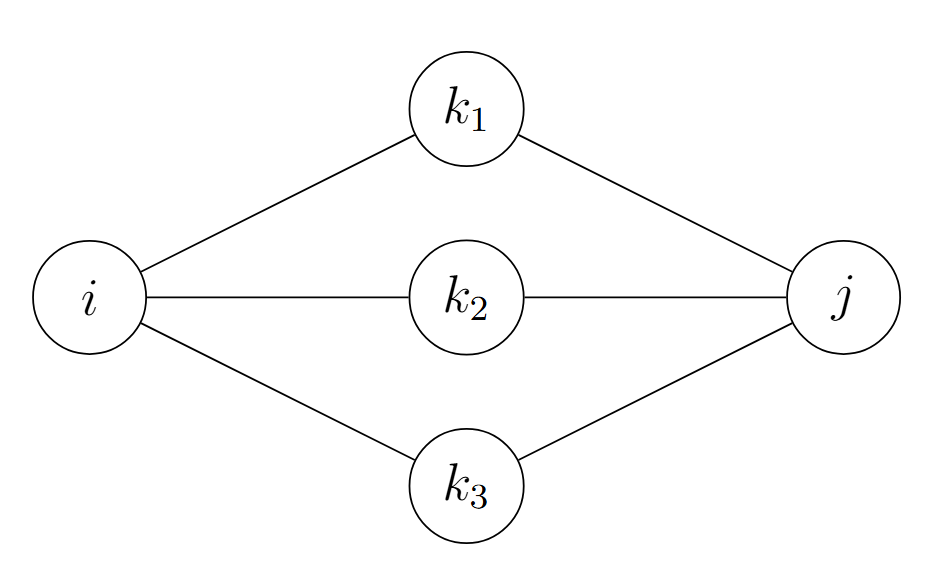
\includegraphics[width=5.72917in,height=\textheight,keepaspectratio]{Imagenes_tesis/chapman-k.png}

}

\caption{\label{fig-chapman}La probabilidad de transición
\(p_{ij}(t+s)\) se obtiene sumando las contribuciones de todos los
posibles estados intermedios \(k\).}

\end{figure}%

Por otro lado, también se tiene la existencia de los HMM categóricos.

\begin{tcolorbox}[enhanced jigsaw, leftrule=.75mm, colback=white, arc=.35mm, coltitle=black, bottomtitle=1mm, colbacktitle=quarto-callout-note-color!10!white, toprule=.15mm, title=\textcolor{quarto-callout-note-color}{\faInfo}\hspace{0.5em}{Nota \ref*{nte-hmm-categorico-1}: Definición (Modelo Oculto de Markov Categórico)}, opacityback=0, left=2mm, toptitle=1mm, titlerule=0mm, rightrule=.15mm, colframe=quarto-callout-note-color-frame, bottomrule=.15mm, breakable, opacitybacktitle=0.6]

\quartocalloutnte{nte-hmm-categorico-1} 

Un Modelo Oculto de Márkov Categórico (Categorical HMM, a menudo también
llamado HMM Discreto o Multinomial) es una variante de los modelos HMM
donde las observaciones emitidas por los estados ocultos son valores
discretos y finitos que pertenecen a categorías específicas, en lugar de
ser valores numéricos continuos.

En cualquier HMM, el sistema modela un proceso estocástico con estados
que no son directamente visibles, y cada estado genera (emite) una
observación que sí podemos medir.

\end{tcolorbox}

\bookmarksetup{startatroot}

\chapter{Dinámica Infinitesimal y Generador de la
Cadena}\label{dinuxe1mica-infinitesimal-y-generador-de-la-cadena}

La evolución continua del color del pixel requiere una descripción
mediante probabilidades de transición, lo cual nos lleva a la
representación matricial de la derivada de \(P(t)\).

\begin{tcolorbox}[enhanced jigsaw, leftrule=.75mm, colback=white, arc=.35mm, coltitle=black, bottomtitle=1mm, colbacktitle=quarto-callout-note-color!10!white, toprule=.15mm, title=\textcolor{quarto-callout-note-color}{\faInfo}\hspace{0.5em}{Nota \ref*{nte-matriz-generadora}: Definición (Matriz Generadora Infinitesimal)}, opacityback=0, left=2mm, toptitle=1mm, titlerule=0mm, rightrule=.15mm, colframe=quarto-callout-note-color-frame, bottomrule=.15mm, breakable, opacitybacktitle=0.6]

\quartocalloutnte{nte-matriz-generadora} 

Asumiendo que \(p_{ij}(t)\) es diferenciable por la derecha en \(t=0\),
definimos la probabilidad de transición \(q_{ij}\) del estado \(i\) al
estado \(j\) (donde \(i \neq j\)) como:

\[
q_{ij}
=
\lim_{h \to 0^+}
\frac{p_{ij}(h)}{h}
\ge 0.
\]

Y para el caso \(i=j\), definimos la probabilidad de salida del estado
\(i\) como \(v_i=-q_{ii}\), dada por

\[
q_{ii}
=
\lim_{h\to0^+}
\frac{p_{ii}(h)-1}{h}
=
-\sum_{j\neq i} q_{ij}
\le 0.
\]

La matriz

\[
Q=[q_{ij}]_{i,j\in S}
\]

se denomina matriz generadora (o matriz \(Q\)) de la cadena. Sus filas
suman cero:

\[
\sum_{j\in S} q_{ij}=0.
\]

\end{tcolorbox}

\begin{tcolorbox}[enhanced jigsaw, leftrule=.75mm, colback=white, arc=.35mm, coltitle=black, bottomtitle=1mm, colbacktitle=quarto-callout-important-color!10!white, toprule=.15mm, title=\textcolor{quarto-callout-important-color}{\faExclamation}\hspace{0.5em}{Importante \ref*{imp-ecuaciones-dif-kolmogorov}: Propiedad (Ecuaciones Diferenciales de Kolmogorov)}, opacityback=0, left=2mm, toptitle=1mm, titlerule=0mm, rightrule=.15mm, colframe=quarto-callout-important-color-frame, bottomrule=.15mm, breakable, opacitybacktitle=0.6]

\quartocalloutimp{imp-ecuaciones-dif-kolmogorov} 

Bajo condiciones de regularidad (que se cumplen trivialmente si el
espacio de estados del color \(S\) es finito), la matriz de transición
\(P(t)\) es la solución única a las ecuaciones diferenciales matriciales
de Kolmogorov Hacia Adelante (Forward) y Hacia Atrás (Backward)
@Norris1998 :

\begin{itemize}
\tightlist
\item
  \textbf{Forward:}
\end{itemize}

\[
\frac{d}{dt}P(t)=P(t)Q
\]

\begin{itemize}
\tightlist
\item
  \textbf{Backward:}
\end{itemize}

\[
\frac{d}{dt}P(t)=QP(t)
\]

Cuya solución formal, bajo la condición inicial \(P(0)=I\) (matriz
identidad), es la matriz exponencial

\[
P(t)
=
e^{Qt}
=
\sum_{n=0}^{\infty}
\frac{(Qt)^n}{n!}.
\]

\end{tcolorbox}

\bookmarksetup{startatroot}

\chapter{Utilidad hacia Cadenas de Márkov Ocultas
(HMM)}\label{utilidad-hacia-cadenas-de-muxe1rkov-ocultas-hmm}

La fundamentación teórica precedente modela la dinámica subyacente
determinista de la matriz de transición y la evolución estocástica de
las trayectorias del sistema. Para extender esta arquitectura a un
Modelo Oculto de Márkov (HMM) en el contexto de la inferencia y análisis
de píxeles en imágenes que contienen letras del alfabeto latino, se
formaliza la siguiente estructura bivariada:

\begin{tcolorbox}[enhanced jigsaw, leftrule=.75mm, colback=white, arc=.35mm, coltitle=black, bottomtitle=1mm, colbacktitle=quarto-callout-note-color!10!white, toprule=.15mm, title=\textcolor{quarto-callout-note-color}{\faInfo}\hspace{0.5em}{Nota \ref*{nte-proceso-latente}: Definición (Proceso Latente e Inobservable)}, opacityback=0, left=2mm, toptitle=1mm, titlerule=0mm, rightrule=.15mm, colframe=quarto-callout-note-color-frame, bottomrule=.15mm, breakable, opacitybacktitle=0.6]

\quartocalloutnte{nte-proceso-latente} 

El proceso de Markov a tiempo continuo

\[
X = \{X(t)\}_{t \ge 0}
\]

sobre el espacio de estados \(S\), caracterizado por su matriz
generadora infinitesimal \(Q\), constituye el \emph{proceso latente}.
Las alteraciones estocásticas inducidas por \(Q\) a lo largo del
parámetro \(t\) (representando una métrica de degradación física o
divergencia espacial) rigen las transiciones hacia estados degradados,
manteniéndose inaccesibles a la medición directa.

\end{tcolorbox}

La variable \(X(t)\) describe el estado ideal o ``verdadero'' del pixel.

\begin{tcolorbox}[enhanced jigsaw, leftrule=.75mm, colback=white, arc=.35mm, coltitle=black, bottomtitle=1mm, colbacktitle=quarto-callout-note-color!10!white, toprule=.15mm, title=\textcolor{quarto-callout-note-color}{\faInfo}\hspace{0.5em}{Nota \ref*{nte-proceso-observacion}: Definición (Proceso de Observación Empírica)}, opacityback=0, left=2mm, toptitle=1mm, titlerule=0mm, rightrule=.15mm, colframe=quarto-callout-note-color-frame, bottomrule=.15mm, breakable, opacitybacktitle=0.6]

\quartocalloutnte{nte-proceso-observacion} 

Sea

\[
(O,\mathcal{P}(O))
\]

el espacio medible de las posibles mediciones obtenidas por
instrumentos.

Se postula un \emph{proceso de observación} acoplado

\[
Y=\{Y(t)\}_{t\ge0},
\]

compuesto por variables aleatorias

\[
Y(t):\Omega\to O
\]

que representan la lectura empírica o ruidosa en el parámetro \(t\).

\end{tcolorbox}

En este caso \(O\) denota el conjunto finito de colores o intensidades
registrables por un sensor óptico y \(Y\) es la lectura ruidosa del
pixel en el tiempo \(t\).

\begin{tcolorbox}[enhanced jigsaw, leftrule=.75mm, colback=white, arc=.35mm, coltitle=black, bottomtitle=1mm, colbacktitle=quarto-callout-note-color!10!white, toprule=.15mm, title=\textcolor{quarto-callout-note-color}{\faInfo}\hspace{0.5em}{Nota \ref*{nte-matriz-emision}: Definición (Matriz de Emisión e Independencia Condicional)}, opacityback=0, left=2mm, toptitle=1mm, titlerule=0mm, rightrule=.15mm, colframe=quarto-callout-note-color-frame, bottomrule=.15mm, breakable, opacitybacktitle=0.6]

\quartocalloutnte{nte-matriz-emision} 

La dependencia estocástica entre ambos procesos queda unívocamente
determinada por la condición de independencia local.

Para cualquier instante \(t\ge0\), la observación \(Y(t)\) es
condicionalmente independiente de toda la historia previa del sistema
dado el estado concurrente \(X(t)\).

Formalmente, para cualquier \(y\in O\) y \(x\in S\):

\[
\mathbb{P}(Y(t)=y \mid \mathcal{F}_t^X,\mathcal{F}_{t^-}^Y)
=
\mathbb{P}(Y(t)=y \mid X(t)=x)
\quad
\text{c.s.}
\]

donde \(\mathcal{F}_t^X\) y \(\mathcal{F}_{t^-}^Y\) denotan las
filtraciones Note~\ref{nte-espacio-filtrado} del historial latente y
observable, respectivamente.

Estas probabilidades definen las entradas de la matriz de emisión
estocástica

\[
E=[e_{xy}],
\]

donde \[
e_{xy}
=
\mathbb{P}(Y(t)=y \mid X(t)=x).
\]

\end{tcolorbox}

\bookmarksetup{startatroot}

\chapter{Inferencia y Filtrado en el Modelo
Oculto}\label{inferencia-y-filtrado-en-el-modelo-oculto}

Una vez establecida la dinámica del sistema, es necesario desarrollar la
maquinaria analítica para inferir el estado latente del pixel a partir
de las observaciones empíricas.

Supongamos que disponemos de una secuencia de observaciones

\[
Y=(y_1,y_2,\dots,y_K)
\]

en instantes discretos de tiempo (o espacio)

\[
0 \le t_1 < t_2 < \dots < t_K \le T.
\]

\begin{tcolorbox}[enhanced jigsaw, leftrule=.75mm, colback=white, arc=.35mm, coltitle=black, bottomtitle=1mm, colbacktitle=quarto-callout-note-color!10!white, toprule=.15mm, title=\textcolor{quarto-callout-note-color}{\faInfo}\hspace{0.5em}{Nota \ref*{nte-filtro-forward}: Definición (Filtro Hacia Adelante (Forward) y Verosimilitud)}, opacityback=0, left=2mm, toptitle=1mm, titlerule=0mm, rightrule=.15mm, colframe=quarto-callout-note-color-frame, bottomrule=.15mm, breakable, opacitybacktitle=0.6]

\quartocalloutnte{nte-filtro-forward} 

Definimos la variable de avance \(\alpha_k(i)\) como la probabilidad
conjunta de observar la secuencia parcial hasta el \(k\)-ésimo instante
y que el estado oculto en dicho instante sea \(i\in S\):

\[
\alpha_k(i)
=
\mathbb{P}
\bigl(
Y(t_1)=y_1,\dots,Y(t_k)=y_k,
X(t_k)=i
\bigr).
\]

Esta cantidad se calcula recursivamente mediante la ecuación de
Chapman-Kolmogorov Important~\ref{imp-chapman-kolmogorov} y la matriz de
emisión \(E\) Note~\ref{nte-matriz-emision}:

\[
\alpha_k(j)
=
\left(
\sum_{i\in S}
\alpha_{k-1}(i)\,
p_{ij}(\Delta t_k)
\right)
\mathbb{P}
\bigl(
Y(t_k)=y_k
\mid
X(t_k)=j
\bigr)
\]

donde

\[
\Delta t_k=t_k-t_{k-1}
\]

y

\[
p_{ij}(\Delta t_k)
\]

es la entrada correspondiente de la matriz de transición

\[
P(\Delta t_k)
=
e^{Q\Delta t_k}.
\]

La verosimilitud total de la secuencia de observaciones es simplemente

\[
\mathbb{P}(Y)
=
\sum_{i\in S}
\alpha_K(i).
\]

\end{tcolorbox}

\begin{tcolorbox}[enhanced jigsaw, leftrule=.75mm, colback=white, arc=.35mm, coltitle=black, bottomtitle=1mm, colbacktitle=quarto-callout-note-color!10!white, toprule=.15mm, title=\textcolor{quarto-callout-note-color}{\faInfo}\hspace{0.5em}{Nota \ref*{nte-decodificacion-optima}: Definición (Decodificación Óptima Global)}, opacityback=0, left=2mm, toptitle=1mm, titlerule=0mm, rightrule=.15mm, colframe=quarto-callout-note-color-frame, bottomrule=.15mm, breakable, opacitybacktitle=0.6]

\quartocalloutnte{nte-decodificacion-optima} 

Para reconstruir la trayectoria más probable, buscamos la secuencia de
estados latentes

\[
\hat{X}
=
(\hat{x}_1,\dots,\hat{x}_K)
\]

que maximice la probabilidad condicional conjunta

\[
\hat{X}
=
\arg\max_{x_1,\dots,x_K}
\mathbb{P}
\Bigl(
X(t_1)=x_1,\dots,X(t_K)=x_K
\mid
Y(t_1)=y_1,\dots,Y(t_K)=y_K
\Bigr).
\]

A diferencia de la función \(\max\), que devuelve el \textbf{valor
numérico} de la probabilidad más alta alcanzada, el operador
\(\arg\max\) (argumento del máximo) devuelve el \textbf{conjunto de
entradas} que producen ese valor máximo. En este contexto, no nos
interesa saber cuál es el porcentaje exacto de la probabilidad máxima,
sino descubrir específicamente \textbf{cuál es la secuencia exacta de
estados latentes} \(\hat{X}\) que hace que esa probabilidad sea máxima

La solución sistemática a este problema de programación dinámica
espacial/temporal se obtiene mediante la adaptación del Algoritmo de
Viterbi @rabiner1989tutorial para cadenas a tiempo continuo, evaluando
las transiciones máximas sobre

\[
P(\Delta t_k).
\]

\end{tcolorbox}

Para los pixeles es la trayectoria más probable de los colores
verdaderos del pixel (el problema de decodificación).

\section{Ejemplo ilustrativo del algoritmo
Forward--Backward}\label{ejemplo-ilustrativo-del-algoritmo-forwardbackward}

Para ilustrar el funcionamiento de los algoritmos Forward y Backward en
el contexto del reconocimiento de imágenes, consideremos un píxel cuyo
color verdadero puede encontrarse en uno de dos estados ocultos:

\[
S=\{B,N\},
\]

donde:

\begin{itemize}
\tightlist
\item
  \(B\): píxel verdaderamente blanco.
\item
  \(N\): píxel verdaderamente negro.
\end{itemize}

Debido al ruido en el proceso de adquisición de la imagen, el color
observado puede diferir del color real.

Supongamos que la dinámica del píxel está descrita por la matriz de
transición

\[
P=
\begin{pmatrix}
0.8 & 0.2\\
0.3 & 0.7
\end{pmatrix},
\]

donde, por ejemplo,

\[
p_{BN}=0.2
\]

representa la probabilidad de que un píxel blanco pase al estado negro
en el siguiente instante.

Asimismo, consideremos la siguiente matriz de emisión:

\[
E=
\begin{pmatrix}
0.9 & 0.1\\
0.2 & 0.8
\end{pmatrix},
\]

cuyas columnas corresponden a las observaciones

\[
(O_B,O_N),
\]

es decir, observar blanco u observar negro. Por ejemplo,

\[
P(O_B \mid B)=0.9,
\qquad
P(O_B \mid N)=0.2.
\]

Finalmente, asumimos una distribución inicial

\[
\pi=(0.6,0.4),
\]

y que la secuencia observada es

\[
Y=(O_B,O_N).
\]

Esto significa que el sensor registra blanco en el primer instante y
negro en el segundo.

\subsection{Cálculo Forward}\label{cuxe1lculo-forward}

La variable Forward se define como

\[
\alpha_k(i)
=
P(y_1,\ldots,y_k,X_k=i).
\]

\subsubsection{Paso 1}\label{paso-1}

Para la primera observación \(O_B\):

\[
\alpha_1(B)
=
P(X_1=B)\,P(O_B\mid B)
=
0.6(0.9)
=
0.54,
\]

\[
\alpha_1(N)
=
P(X_1=N)\,P(O_B\mid N)
=
0.4(0.2)
=
0.08.
\]

\subsubsection{Paso 2}\label{paso-2}

Calculamos primero la probabilidad de alcanzar el estado blanco:

\[
\sum_{i\in S}
\alpha_1(i)p_{iB}
=
0.54(0.8)+0.08(0.3)
=
0.456.
\]

Multiplicando por la probabilidad de emisión correspondiente,

\[
\alpha_2(B)
=
0.456(0.1)
=
0.0456.
\]

Análogamente, para el estado negro:

\[
\sum_{i\in S}
\alpha_1(i)p_{iN}
=
0.54(0.2)+0.08(0.7)
=
0.164,
\]

y por tanto,

\[
\alpha_2(N)
=
0.164(0.8)
=
0.1312.
\]

\subsubsection{Verosimilitud de la secuencia
observada}\label{verosimilitud-de-la-secuencia-observada}

La probabilidad total de observar la secuencia \(Y\) es

\[
P(Y)
=
\alpha_2(B)+\alpha_2(N),
\]

es decir,

\[
P(Y)
=
0.0456+0.1312
=
0.1768.
\]

\subsection{Cálculo Backward}\label{cuxe1lculo-backward}

La variable Backward se define mediante

\[
\beta_k(i)
=
P(y_{k+1},\ldots,y_T\mid X_k=i).
\]

Como la secuencia contiene únicamente dos observaciones,

\[
\beta_2(B)=\beta_2(N)=1.
\]

Retrocediendo un paso:

\[
\beta_1(B)
=
0.8(0.1)(1)
+
0.2(0.8)(1)
=
0.24,
\]

y

\[
\beta_1(N)
=
0.3(0.1)(1)
+
0.7(0.8)(1)
=
0.59.
\]

\subsection{Inferencia del estado
oculto}\label{inferencia-del-estado-oculto}

Una de las principales ventajas del algoritmo Forward--Backward es que
permite calcular la probabilidad posterior de cada estado oculto.

Para el estado blanco en el primer instante,

\[
\gamma_1(B)
=
P(X_1=B\mid Y)
=
\frac{\alpha_1(B)\beta_1(B)}
{P(Y)},
\]

por lo que

\[
\gamma_1(B)
=
\frac{0.54(0.24)}
{0.1768}
=
0.733.
\]

De forma análoga,

\[
\gamma_1(N)
=
\frac{\alpha_1(N)\beta_1(N)}
{P(Y)}
=
\frac{0.08(0.59)}
{0.1768}
=
0.267.
\]

En consecuencia,

\[
P(X_1=B\mid Y)\approx 73.3\%,
\]

mientras que

\[
P(X_1=N\mid Y)\approx 26.7\%.
\]

\textbf{Interpretación}

A pesar de que el sensor observa un píxel blanco en el primer instante y
negro en el segundo, el algoritmo Forward--Backward determina que existe
aproximadamente un \(73\%\) de probabilidad de que el color verdadero
inicial haya sido blanco. Este resultado muestra cómo un Modelo Oculto
de Markov combina la información proporcionada por las observaciones
ruidosas con la dinámica de transición del sistema para inferir el
estado real subyacente del píxel.

\begin{figure}

\centering{

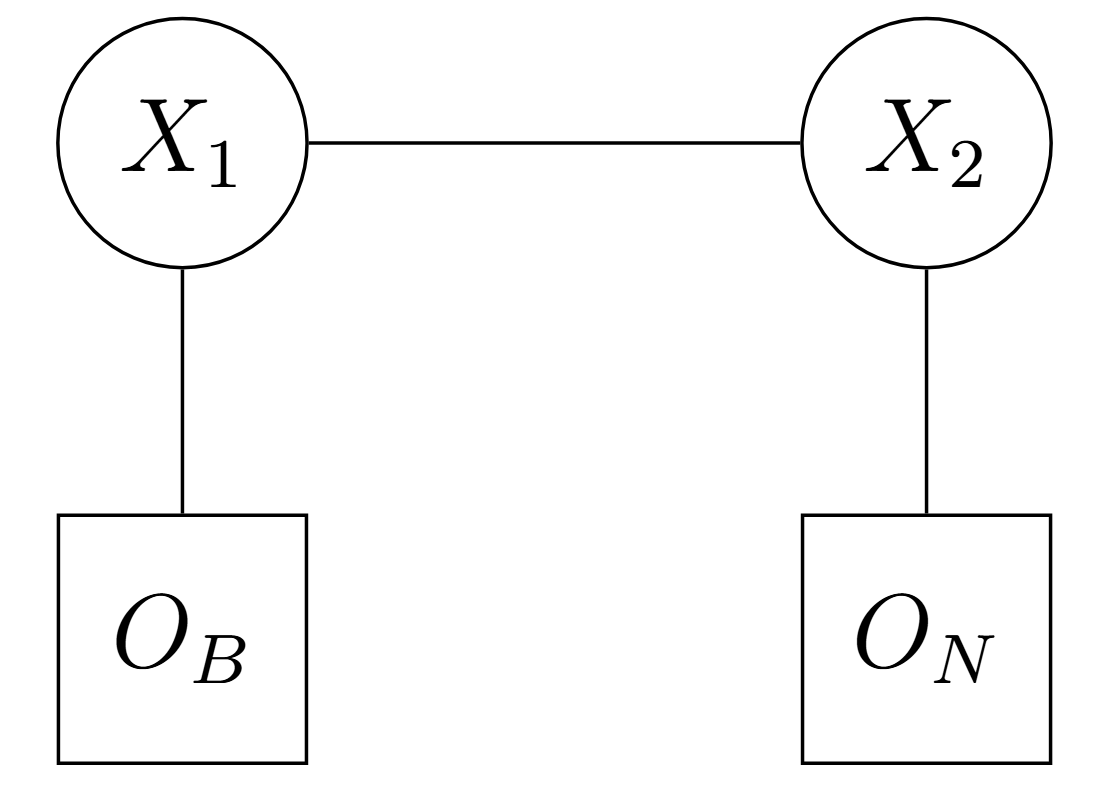
\includegraphics[width=4.6875in,height=\textheight,keepaspectratio]{images/imagenesHMM/pixelblanconegrodibujo.png}

}

\caption{\label{fig-pixelbn}Modelo Oculto de Markov para un píxel con
dos estados ocultos y dos observaciones.}

\end{figure}%

\bookmarksetup{startatroot}

\chapter{Estimación de Parámetros y Calibración del
Modelo}\label{estimaciuxf3n-de-paruxe1metros-y-calibraciuxf3n-del-modelo}

En la práctica, la matriz generadora infinitesimal \(Q\) (que dicta la
probabilidad de degradación del color para el caso de estudio) y las
probabilidades de emisión empírica rara vez son conocidas a priori y
deben ser estimadas a partir de un dataset de imágenes (el alfabeto
latino modificado).

\begin{tcolorbox}[enhanced jigsaw, leftrule=.75mm, colback=white, arc=.35mm, coltitle=black, bottomtitle=1mm, colbacktitle=quarto-callout-important-color!10!white, toprule=.15mm, title=\textcolor{quarto-callout-important-color}{\faExclamation}\hspace{0.5em}{Importante \ref*{nte-baum-welch}: Propiedad (Algoritmo de Expectation-Maximization (Baum-Welch))}, opacityback=0, left=2mm, toptitle=1mm, titlerule=0mm, rightrule=.15mm, colframe=quarto-callout-important-color-frame, bottomrule=.15mm, breakable, opacitybacktitle=0.6]

\quartocalloutnte{nte-baum-welch} 

La estimación por máxima verosimilitud del conjunto de parámetros del
modelo

\[
\Theta=\{Q,E\}
\]

dado un conjunto de secuencias observadas se realiza mediante un proceso
iterativo.

\begin{itemize}
\item
  \textbf{Paso} \(E\) (\textbf{Expectation):} Se calculan las
  estadísticas suficientes esperadas del sistema latente (tiempo
  esperado de permanencia en cada estado de color y número esperado de
  transiciones) condicionado a las observaciones y a la estimación
  actual de los parámetros en el paso \(m\) \(\Theta^{(m)}\), utilizando
  las variables recursivas Forward y Backward.
\item
  \textbf{Paso} \(M\) \textbf{(Maximization):} Se actualizan los
  parámetros \(\Theta^{(m+1)}\) para maximizar la función \(Q\) de
  verosimilitud esperada. En particular, la estimación de las
  probabilidades de transición empíricas se formula restringiendo las
  soluciones para garantizar que las filas de \(Q^{(m+1)}\) sigan
  sumando cero y \(q_{ij}\ge0\) para \(i\neq j\).
\end{itemize}

\end{tcolorbox}

\begin{figure}

\centering{

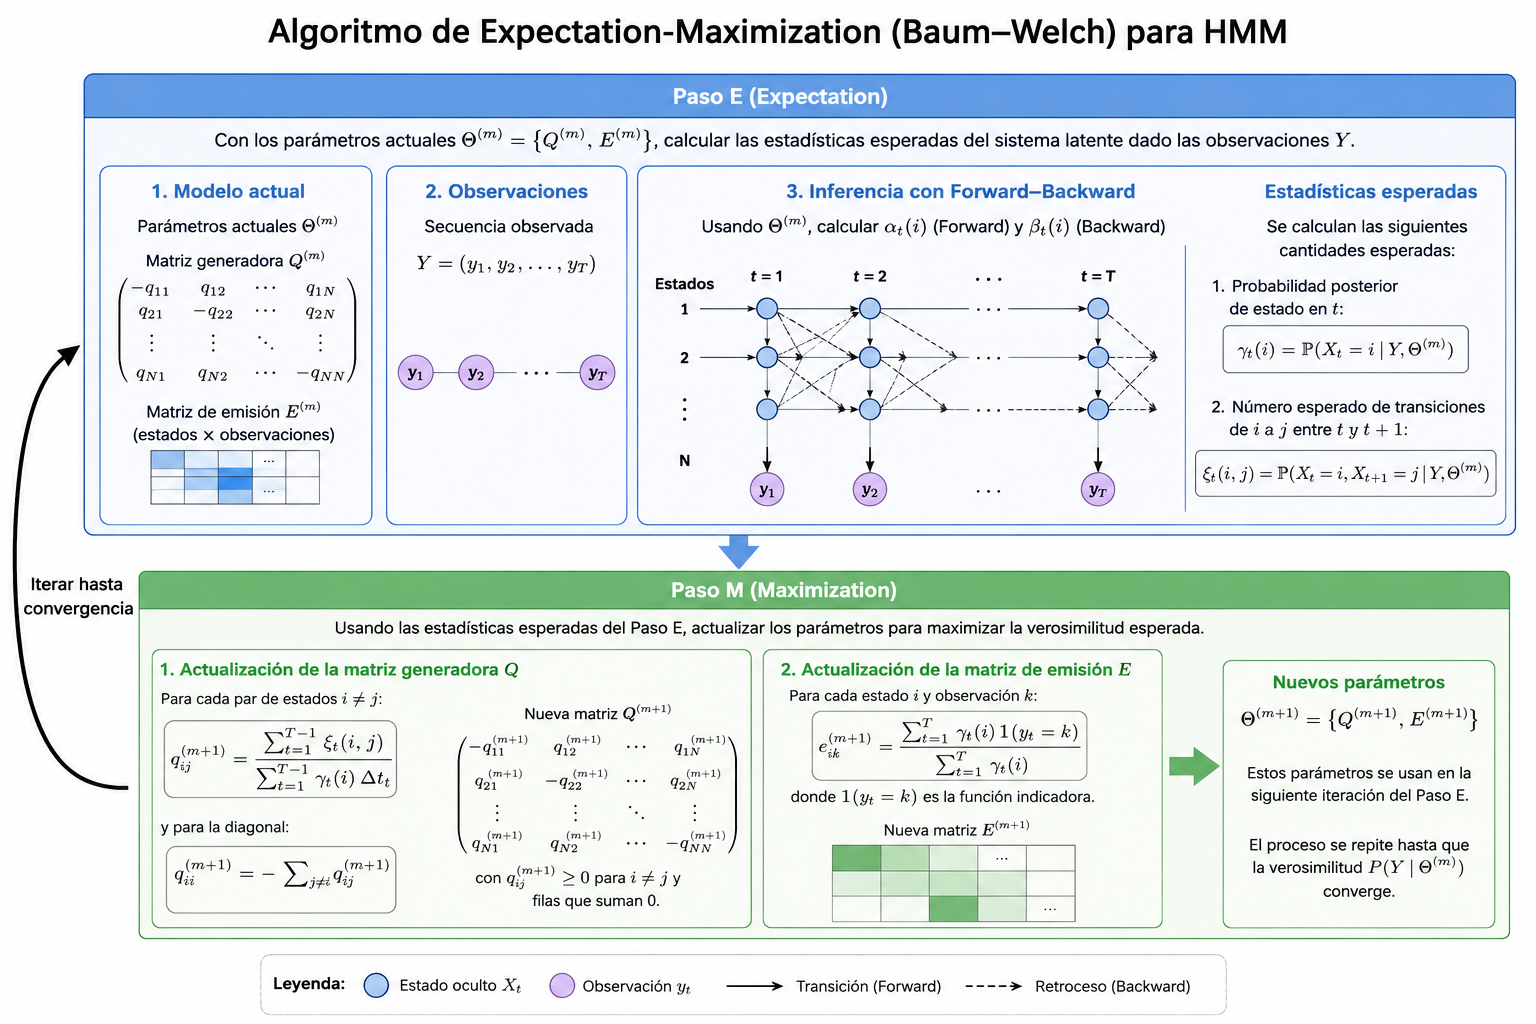
\includegraphics[width=5.20833in,height=\textheight,keepaspectratio]{images/imagenesHMM/ME_HMM.png}

}

\caption{\label{fig-ME}Esquema general del algoritmo
Expectation--Maximization (Baum--Welch) para un Modelo Oculto de Markov.
En el Paso E se estiman las probabilidades posteriores de los estados
ocultos y las transiciones esperadas mediante los algoritmos
Forward--Backward. En el Paso M se actualizan iterativamente la matriz
generadora y la matriz de emisión para maximizar la verosimilitud de las
observaciones.}

\end{figure}%

\bookmarksetup{startatroot}

\chapter{Base de datos}\label{base-de-datos}

\section{Construcción del conjunto de
datos}\label{construcciuxf3n-del-conjunto-de-datos}

El reconocimiento óptico de caracteres para sistemas de escritura
indígenas, particularmente para el alfabeto Náhuatl
Figura~\ref{fig-alfabeto-nahuatl}, presenta una limitación inicial
importante: no existe un conjunto de datos público, estandarizado y
etiquetado que permita entrenar modelos de aprendizaje profundo. A
diferencia de otros alfabetos, para los cuales existen repositorios
ampliamente documentados, el alfabeto Náhuatl carece de recursos
computacionales que puedan emplearse directamente en tareas de
clasificación automática.

\begin{figure}

\centering{

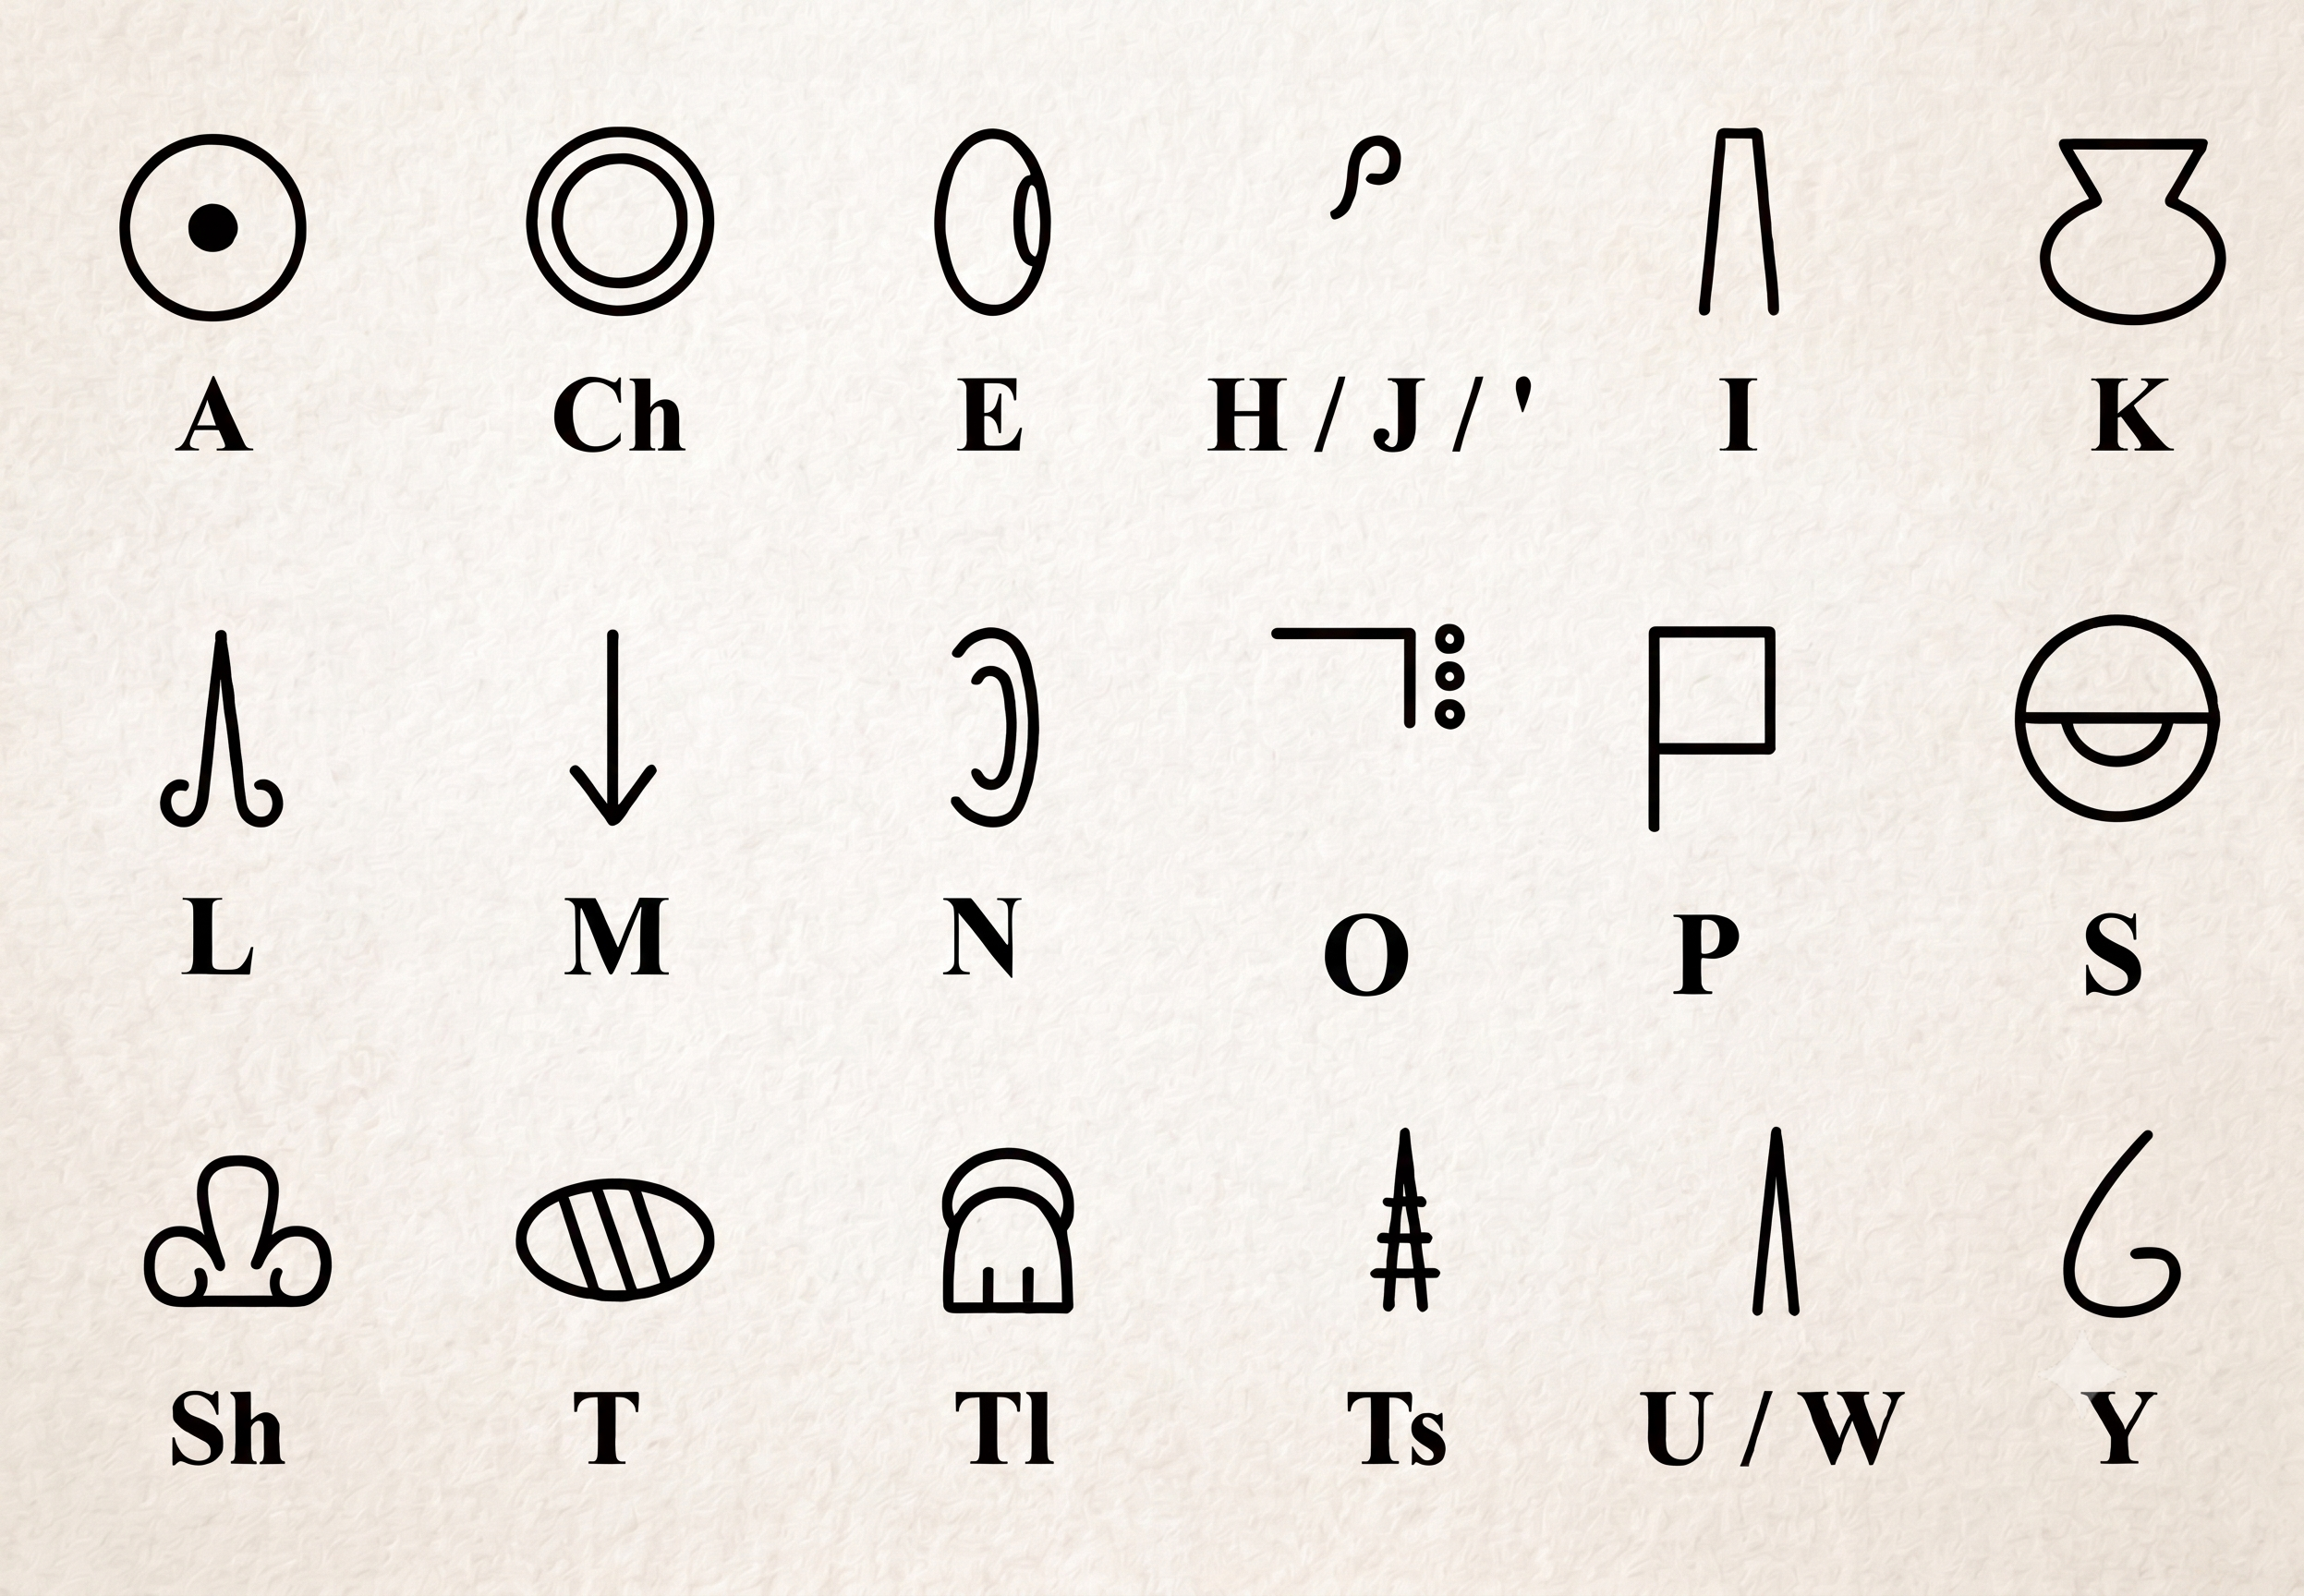
\includegraphics[width=8.33333in,height=\textheight,keepaspectratio]{images/Alfabeto nahuatl.png}

}

\caption{\label{fig-alfabeto-nahuatl}Glifos del alfabeto nahuatl. Este
alfabeto consta de 18 caracteres, para los cuales se emplean letras del
alfabeto latino para su manipulación.}

\end{figure}%

Ante esta situación, fue necesario construir un conjunto de datos
propio. La decisión de generar un dataset sintético se tomó por dos
razones principales:

\begin{enumerate}
\def\labelenumi{\arabic{enumi}.}
\tightlist
\item
  Proporcionar un número suficiente de ejemplos para el entrenamiento de
  la red neuronal.
\item
  Introducir variaciones geométricas que permitan al modelo generalizar
  ante deformaciones presentes en documentos reales.
\end{enumerate}

\subsection{Generación de las
muestras}\label{generaciuxf3n-de-las-muestras}

Inicialmente se diseñaron de forma manual 25 ejemplos base para cada
carácter del alfabeto. Posteriormente, a cada muestra se le aplicaron
transformaciones geométricas y perturbaciones aleatorias para
incrementar la variabilidad del conjunto de datos.

La Figura Figura~\ref{fig-dataset-augmentation} muestra algunos ejemplos
de las imágenes generadas.

\begin{figure}

\centering{

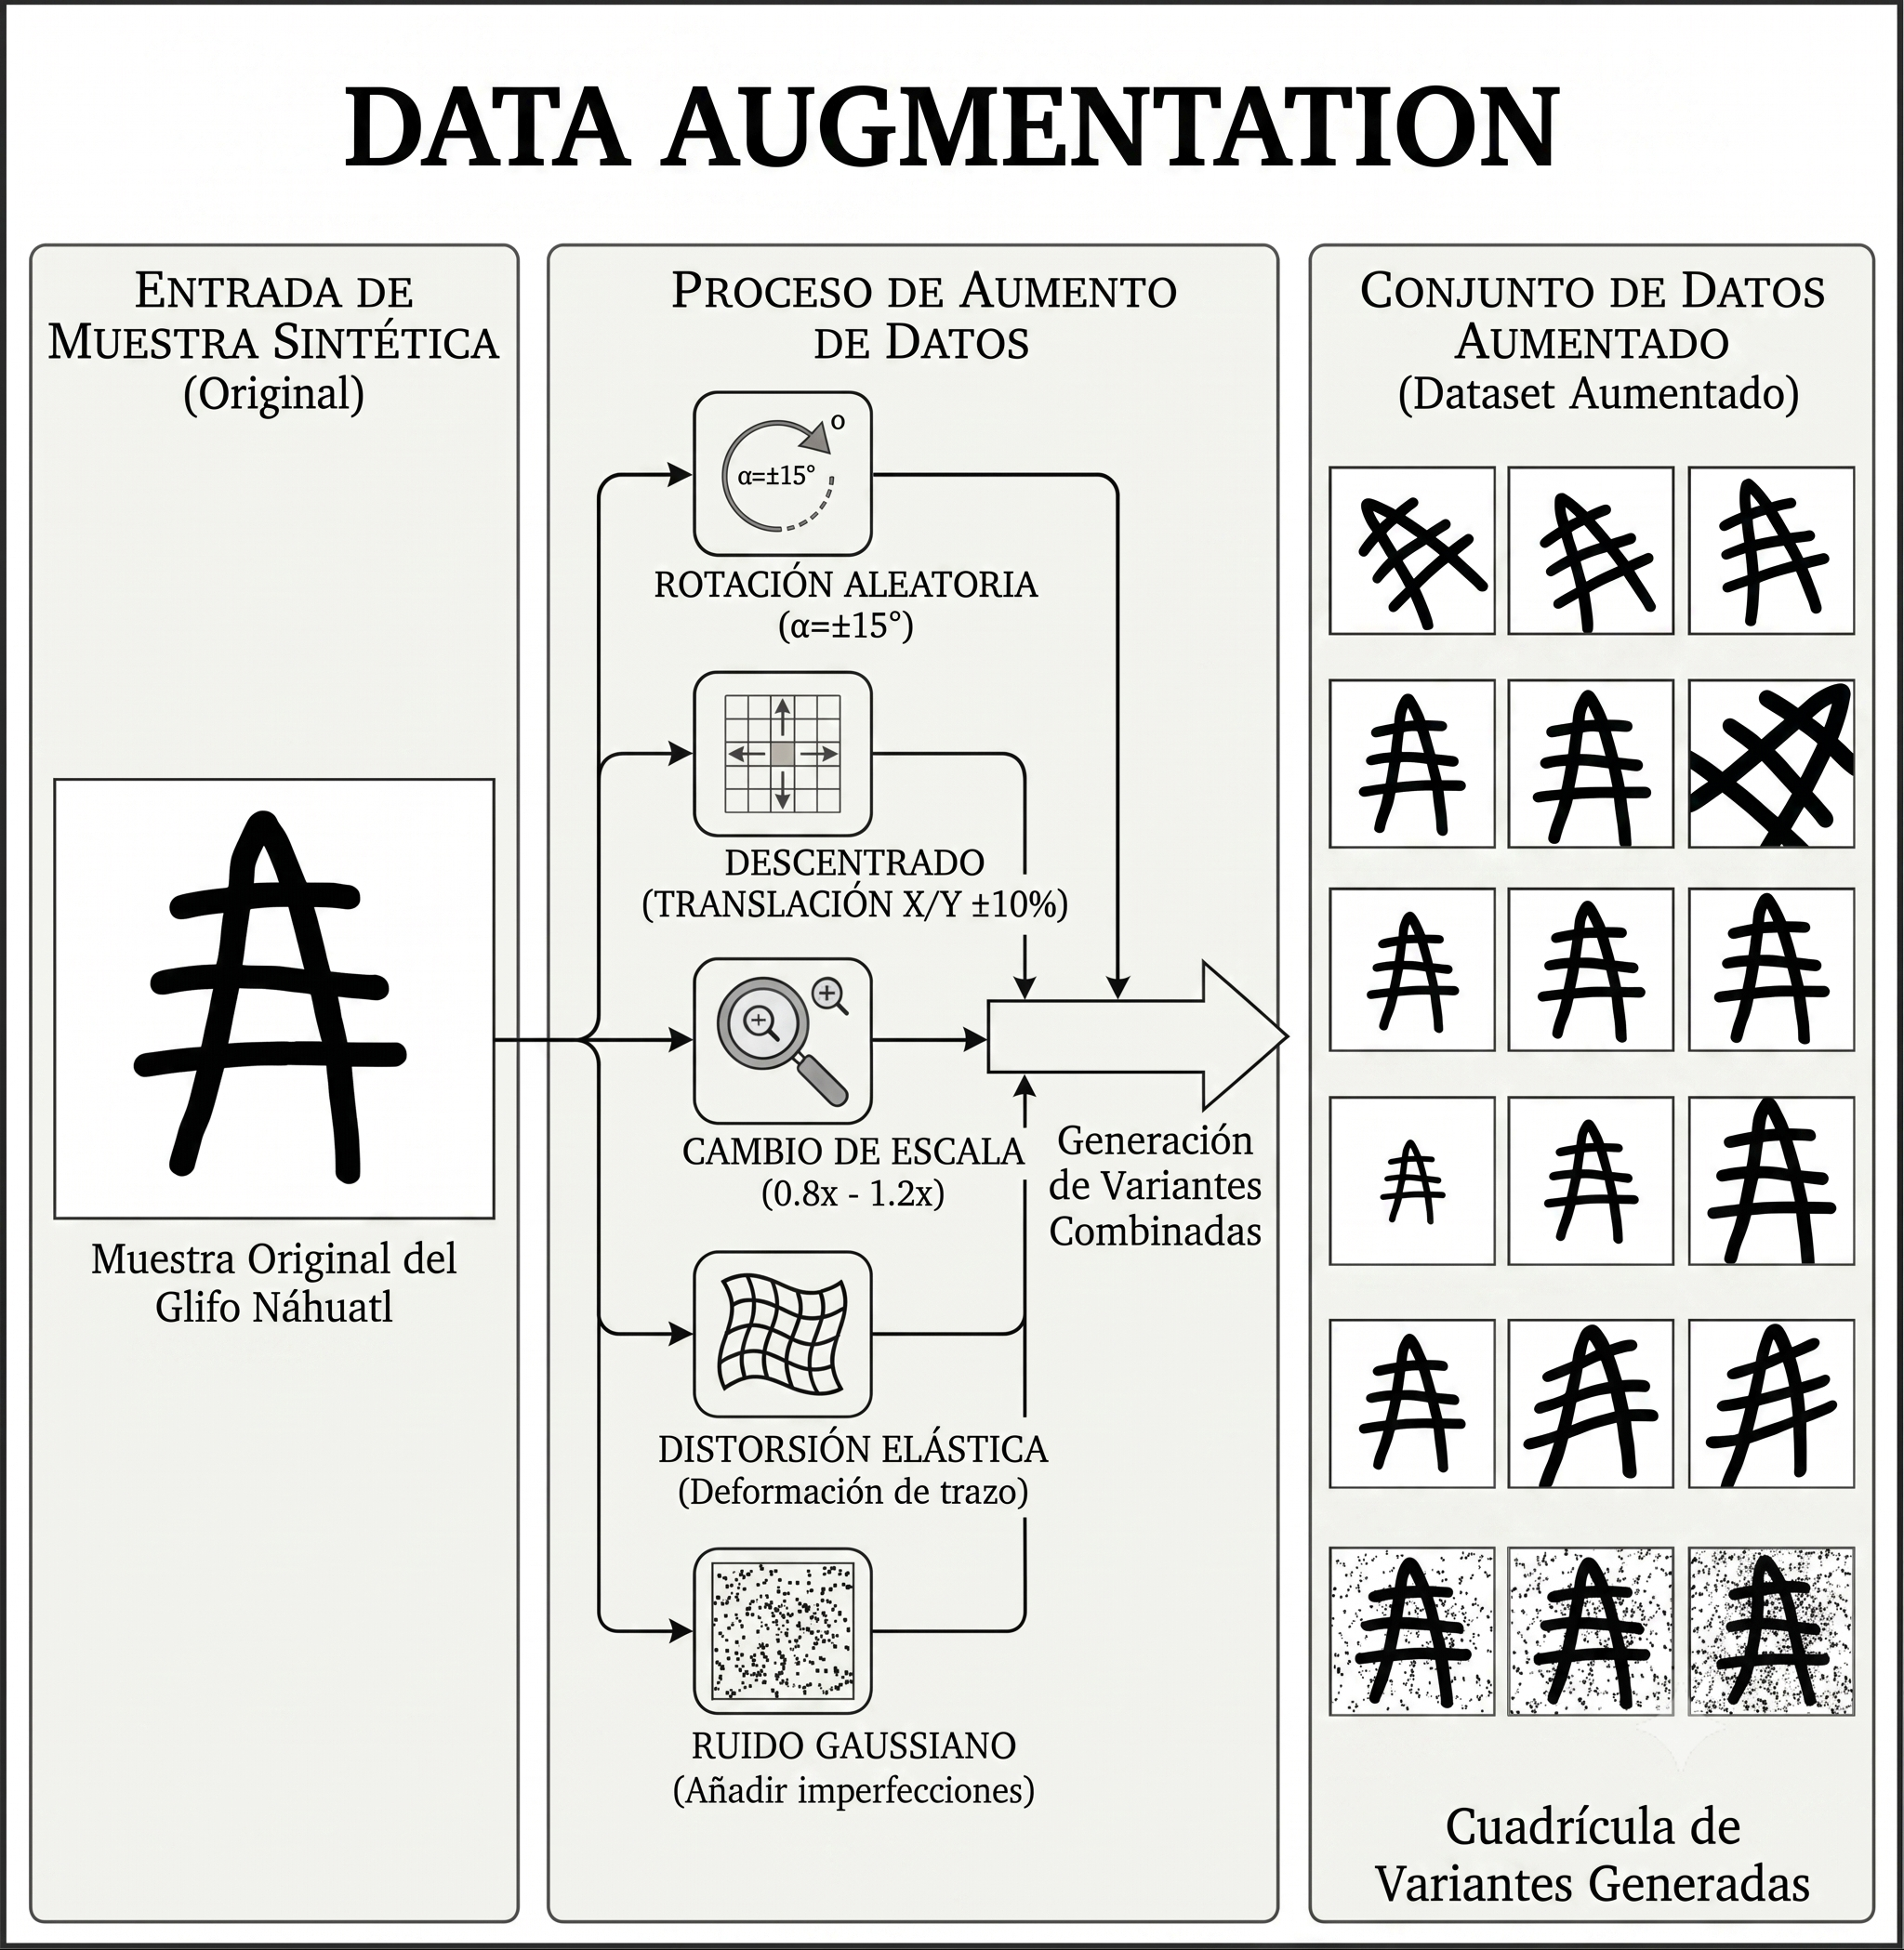
\includegraphics[width=8.33333in,height=\textheight,keepaspectratio]{images/dataset aumentado.png}

}

\caption{\label{fig-dataset-augmentation}Se observa el proceso por el
que pasa cada una de las 25 imagenes por letra para generar 90 variantes
obtenidas a partir de rotación, traslación, distorción elástica, cambio
de escala y ruido, de este modo se consigue un dataset más completo.}

\end{figure}%

\section{Carga y organización de los
datos}\label{carga-y-organizaciuxf3n-de-los-datos}

Una vez construido el conjunto de datos, las imágenes se almacenaron
siguiendo una estructura jerárquica de directorios, donde cada carpeta
representa una clase distinta del alfabeto.

El cargado de las imágenes se realizó mediante la función
\texttt{image\_dataset\_from\_directory} de TensorFlow:

\begin{Shaded}
\begin{Highlighting}[]
\NormalTok{train\_ds }\OperatorTok{=}\NormalTok{ tf.keras.utils.image\_dataset\_from\_directory(}
\NormalTok{    data\_dir,}
\NormalTok{    validation\_split}\OperatorTok{=}\FloatTok{0.2}\NormalTok{,}
\NormalTok{    subset}\OperatorTok{=}\StringTok{"training"}\NormalTok{,}
\NormalTok{    seed}\OperatorTok{=}\DecValTok{123}\NormalTok{,}
\NormalTok{    image\_size}\OperatorTok{=}\NormalTok{(}\DecValTok{28}\NormalTok{,}\DecValTok{28}\NormalTok{),}
\NormalTok{    batch\_size}\OperatorTok{=}\DecValTok{32}\NormalTok{,}
\NormalTok{    color\_mode}\OperatorTok{=}\StringTok{"grayscale"}
\NormalTok{)}

\NormalTok{val\_ds }\OperatorTok{=}\NormalTok{ tf.keras.utils.image\_dataset\_from\_directory(}
\NormalTok{    data\_dir,}
\NormalTok{    validation\_split}\OperatorTok{=}\FloatTok{0.2}\NormalTok{,}
\NormalTok{    subset}\OperatorTok{=}\StringTok{"validation"}\NormalTok{,}
\NormalTok{    seed}\OperatorTok{=}\DecValTok{123}\NormalTok{,}
\NormalTok{    image\_size}\OperatorTok{=}\NormalTok{(}\DecValTok{28}\NormalTok{,}\DecValTok{28}\NormalTok{),}
\NormalTok{    batch\_size}\OperatorTok{=}\DecValTok{32}\NormalTok{,}
\NormalTok{    color\_mode}\OperatorTok{=}\StringTok{"grayscale"}
\NormalTok{)}
\end{Highlighting}
\end{Shaded}

La elección de una partición de entrenamiento-validación de 80\%-20\%
constituye una práctica común en aprendizaje automático, ya que permite
disponer de un número suficiente de ejemplos para el ajuste de los
parámetros del modelo y, al mismo tiempo, reservar un conjunto
independiente para evaluar la capacidad de generalización.

Asimismo, las imágenes se convirtieron a escala de grises. Dado que los
glifos del alfabeto Náhuatl se distinguen principalmente por su
geometría y no por información cromática, el uso de un solo canal reduce
el costo computacional sin sacrificar información relevante.

\section{Normalización y aumentación de
datos}\label{normalizaciuxf3n-y-aumentaciuxf3n-de-datos}

Antes de alimentar las imágenes a la red neuronal, se realizó un proceso
de normalización:

\begin{Shaded}
\begin{Highlighting}[]
\NormalTok{normalization\_layer }\OperatorTok{=}\NormalTok{ tf.keras.layers.Rescaling(}\FloatTok{1.}\OperatorTok{/}\DecValTok{255}\NormalTok{)}
\end{Highlighting}
\end{Shaded}

Esta transformación reescala los valores de intensidad al intervalo
\([0,1]\), lo cual mejora la estabilidad numérica del proceso de
entrenamiento y facilita la convergencia del algoritmo de optimización.

Adicionalmente, se implementó un mecanismo de aumentación de datos en
línea:

\begin{Shaded}
\begin{Highlighting}[]
\NormalTok{data\_augmentation }\OperatorTok{=}\NormalTok{ tf.keras.Sequential([}
\NormalTok{    tf.keras.layers.RandomRotation(}\FloatTok{0.05}\NormalTok{),}
\NormalTok{    tf.keras.layers.RandomZoom(}\FloatTok{0.1}\NormalTok{),}
\NormalTok{    tf.keras.layers.RandomTranslation(}\FloatTok{0.05}\NormalTok{, }\FloatTok{0.05}\NormalTok{)}
\NormalTok{])}
\end{Highlighting}
\end{Shaded}

La introducción de pequeñas rotaciones, cambios de escala y traslaciones
tiene como objetivo simular las variaciones presentes en documentos
escaneados o en la escritura manual. De esta manera, el modelo aprende
representaciones más robustas y reduce su tendencia al sobreajuste.

Finalmente, los datos fueron almacenados temporalmente en memoria y
preparados para alimentar la GPU:

\begin{Shaded}
\begin{Highlighting}[]
\NormalTok{train\_ds }\OperatorTok{=}\NormalTok{ train\_ds.cache().shuffle(}\DecValTok{5000}\NormalTok{).prefetch(AUTOTUNE)}
\NormalTok{val\_ds }\OperatorTok{=}\NormalTok{ val\_ds.cache().prefetch(AUTOTUNE)}
\end{Highlighting}
\end{Shaded}

El uso de \texttt{cache()} evita que las imágenes sean leídas
repetidamente desde el disco, mientras que \texttt{prefetch()} permite
superponer las operaciones de lectura de datos con el entrenamiento de
la red, disminuyendo el tiempo total de ejecución.

\bookmarksetup{startatroot}

\chapter{Caso de estudio}\label{caso-de-estudio}

\bookmarksetup{startatroot}

\chapter{CASO CNN}\label{caso-cnn}

\section{Arquitectura de la red neuronal
convolucional}\label{arquitectura-de-la-red-neuronal-convolucional}

La arquitectura propuesta recibe imágenes de tamaño
\(28\times28\times1\) y está compuesta por tres bloques convolucionales
seguidos de un clasificador denso.

\begin{Shaded}
\begin{Highlighting}[]
\NormalTok{model }\OperatorTok{=}\NormalTok{ tf.keras.Sequential([}
\NormalTok{    tf.keras.layers.Input(shape}\OperatorTok{=}\NormalTok{(}\DecValTok{28}\NormalTok{,}\DecValTok{28}\NormalTok{,}\DecValTok{1}\NormalTok{)),}

\NormalTok{    tf.keras.layers.Conv2D(}\DecValTok{32}\NormalTok{,}\DecValTok{3}\NormalTok{,activation}\OperatorTok{=}\StringTok{\textquotesingle{}relu\textquotesingle{}}\NormalTok{),}
\NormalTok{    tf.keras.layers.BatchNormalization(),}
\NormalTok{    tf.keras.layers.MaxPooling2D(),}
\NormalTok{    tf.keras.layers.SpatialDropout2D(}\FloatTok{0.25}\NormalTok{),}

\NormalTok{    tf.keras.layers.Conv2D(}\DecValTok{64}\NormalTok{,}\DecValTok{3}\NormalTok{,activation}\OperatorTok{=}\StringTok{\textquotesingle{}relu\textquotesingle{}}\NormalTok{),}
\NormalTok{    tf.keras.layers.BatchNormalization(),}
\NormalTok{    tf.keras.layers.MaxPooling2D(),}
\NormalTok{    tf.keras.layers.SpatialDropout2D(}\FloatTok{0.25}\NormalTok{),}

\NormalTok{    tf.keras.layers.Conv2D(}\DecValTok{128}\NormalTok{,}\DecValTok{3}\NormalTok{,activation}\OperatorTok{=}\StringTok{\textquotesingle{}relu\textquotesingle{}}\NormalTok{),}
\NormalTok{    tf.keras.layers.MaxPooling2D(),}
\NormalTok{    tf.keras.layers.SpatialDropout2D(}\FloatTok{0.25}\NormalTok{),}

\NormalTok{    tf.keras.layers.Flatten(),}
\NormalTok{    tf.keras.layers.Dense(}\DecValTok{256}\NormalTok{, activation}\OperatorTok{=}\StringTok{\textquotesingle{}relu\textquotesingle{}}\NormalTok{),}
\NormalTok{    tf.keras.layers.Dropout(}\FloatTok{0.5}\NormalTok{),}
\NormalTok{    tf.keras.layers.Dense(num\_classes, activation}\OperatorTok{=}\StringTok{\textquotesingle{}softmax\textquotesingle{}}\NormalTok{)}
\NormalTok{])}
\end{Highlighting}
\end{Shaded}

\section{Primer bloque convolucional}\label{primer-bloque-convolucional}

La primera capa convolucional emplea 32 filtros de tamaño \(3\times3\):

\begin{Shaded}
\begin{Highlighting}[]
\NormalTok{tf.keras.layers.Conv2D(}\DecValTok{32}\NormalTok{,}\DecValTok{3}\NormalTok{,activation}\OperatorTok{=}\StringTok{\textquotesingle{}relu\textquotesingle{}}\NormalTok{)}
\end{Highlighting}
\end{Shaded}

Este bloque se encarga de detectar características de bajo nivel, tales
como bordes, esquinas y pequeños segmentos de los trazos.

La incorporación de una capa de normalización por lotes:

\begin{Shaded}
\begin{Highlighting}[]
\NormalTok{tf.keras.layers.BatchNormalization()}
\end{Highlighting}
\end{Shaded}

permite estabilizar la distribución de las activaciones internas,
acelerando el proceso de convergencia.

Posteriormente, la operación de \emph{max pooling}

\begin{Shaded}
\begin{Highlighting}[]
\NormalTok{tf.keras.layers.MaxPooling2D()}
\end{Highlighting}
\end{Shaded}

reduce la dimensionalidad espacial de las representaciones, disminuyendo
el número de parámetros y haciendo al modelo menos sensible a pequeñas
traslaciones.

Finalmente, se incorpora un mecanismo de regularización:

\begin{Shaded}
\begin{Highlighting}[]
\NormalTok{tf.keras.layers.SpatialDropout2D(}\FloatTok{0.25}\NormalTok{)}
\end{Highlighting}
\end{Shaded}

que desactiva mapas de características completos de manera aleatoria,
obligando a la red a aprender representaciones más robustas.

\section{Segundo y tercer bloque
convolucional}\label{segundo-y-tercer-bloque-convolucional}

Los bloques posteriores incrementan progresivamente el número de filtros
hasta 64 y 128, respectivamente. El aumento en la profundidad de la red
permite capturar patrones cada vez más complejos, tales como
combinaciones de curvas, intersecciones y configuraciones geométricas
características de cada glifo.

\section{Clasificador}\label{clasificador}

Las características extraídas se transforman en un vector
unidimensional:

\begin{Shaded}
\begin{Highlighting}[]
\NormalTok{tf.keras.layers.Flatten()}
\end{Highlighting}
\end{Shaded}

y posteriormente se procesan mediante una capa densa:

\begin{Shaded}
\begin{Highlighting}[]
\NormalTok{tf.keras.layers.Dense(}\DecValTok{256}\NormalTok{, activation}\OperatorTok{=}\StringTok{\textquotesingle{}relu\textquotesingle{}}\NormalTok{)}
\end{Highlighting}
\end{Shaded}

La capa de salida utiliza la función Softmax:

\begin{Shaded}
\begin{Highlighting}[]
\NormalTok{tf.keras.layers.Dense(num\_classes, activation}\OperatorTok{=}\StringTok{\textquotesingle{}softmax\textquotesingle{}}\NormalTok{)}
\end{Highlighting}
\end{Shaded}

la cual produce una distribución de probabilidad sobre todas las clases
del alfabeto.

\bookmarksetup{startatroot}

\chapter{Entrenamiento}\label{entrenamiento-1}

El modelo se compiló utilizando el optimizador Adam:

\begin{Shaded}
\begin{Highlighting}[]
\NormalTok{model.}\BuiltInTok{compile}\NormalTok{(}
\NormalTok{    optimizer}\OperatorTok{=}\StringTok{\textquotesingle{}adam\textquotesingle{}}\NormalTok{,}
\NormalTok{    loss}\OperatorTok{=}\StringTok{\textquotesingle{}sparse\_categorical\_crossentropy\textquotesingle{}}\NormalTok{,}
\NormalTok{    metrics}\OperatorTok{=}\NormalTok{[}\StringTok{\textquotesingle{}accuracy\textquotesingle{}}\NormalTok{]}
\NormalTok{)}
\end{Highlighting}
\end{Shaded}

La función de pérdida de entropía cruzada dispersa se seleccionó debido
a que las etiquetas de las imágenes se encuentran codificadas como
enteros y no mediante vectores \emph{one-hot}.

Para evitar el sobreajuste se implementó un mecanismo de detención
temprana:

\begin{Shaded}
\begin{Highlighting}[]
\NormalTok{early\_stop }\OperatorTok{=}\NormalTok{ EarlyStopping(}
\NormalTok{    monitor}\OperatorTok{=}\StringTok{\textquotesingle{}val\_loss\textquotesingle{}}\NormalTok{,}
\NormalTok{    patience}\OperatorTok{=}\DecValTok{7}\NormalTok{,}
\NormalTok{    restore\_best\_weights}\OperatorTok{=}\VariableTok{True}
\NormalTok{)}
\end{Highlighting}
\end{Shaded}

La elección de siete épocas de paciencia permite al modelo continuar el
aprendizaje ante pequeñas oscilaciones de la pérdida de validación,
evitando finalizar el entrenamiento de forma prematura.

Asimismo, el mejor modelo obtenido se almacenó automáticamente:

\begin{Shaded}
\begin{Highlighting}[]
\NormalTok{checkpoint }\OperatorTok{=}\NormalTok{ ModelCheckpoint(}
\NormalTok{    ruta\_modelo,}
\NormalTok{    monitor}\OperatorTok{=}\StringTok{\textquotesingle{}val\_loss\textquotesingle{}}\NormalTok{,}
\NormalTok{    save\_best\_only}\OperatorTok{=}\VariableTok{True}
\NormalTok{)}
\end{Highlighting}
\end{Shaded}

\bookmarksetup{startatroot}

\chapter{Sistema de inferencia
interactivo}\label{sistema-de-inferencia-interactivo}

Finalmente, se desarrolló una interfaz interactiva en Google Colab que
permite dibujar caracteres del alfabeto Náhuatl y obtener predicciones
en tiempo real.

La imagen generada por el usuario se redimensiona a \(28\times28\)
píxeles:

\begin{Shaded}
\begin{Highlighting}[]
\NormalTok{img\_resized }\OperatorTok{=}\NormalTok{ cv2.resize(img, (}\DecValTok{28}\NormalTok{,}\DecValTok{28}\NormalTok{))}
\NormalTok{img\_normalized }\OperatorTok{=}\NormalTok{ img\_resized }\OperatorTok{/} \FloatTok{255.0}
\NormalTok{img\_input }\OperatorTok{=}\NormalTok{ np.expand\_dims(img\_normalized, axis}\OperatorTok{=}\NormalTok{(}\DecValTok{0}\NormalTok{,}\OperatorTok{{-}}\DecValTok{1}\NormalTok{))}
\end{Highlighting}
\end{Shaded}

Posteriormente, el modelo produce un vector de probabilidades:

\begin{Shaded}
\begin{Highlighting}[]
\NormalTok{predicciones }\OperatorTok{=}\NormalTok{ model.predict(img\_input)}
\end{Highlighting}
\end{Shaded}

y se determina la clase más probable mediante:

\begin{Shaded}
\begin{Highlighting}[]
\NormalTok{idx\_ganador }\OperatorTok{=}\NormalTok{ np.argmax(predicciones)}
\end{Highlighting}
\end{Shaded}

Además de la predicción principal, la interfaz presenta las tres clases
con mayor probabilidad, proporcionando información adicional sobre la
confianza y las posibles ambigüedades del modelo.

\bookmarksetup{startatroot}

\chapter{CASO HMM}\label{caso-hmm}

\bookmarksetup{startatroot}

\chapter{Conclusiones: Comparación entre HMM y CNN en Reconocimiento de
Caracteres}\label{conclusiones-comparaciuxf3n-entre-hmm-y-cnn-en-reconocimiento-de-caracteres}

\section{Conclusiones}\label{conclusiones}

La comparación entre los modelos ocultos de Markov (HMM) y las redes
neuronales convolucionales (CNN) en el reconocimiento de caracteres
evidencia un cambio de paradigma fundamental en el procesamiento de
imágenes. La diferencia más significativa radica en el proceso de
extracción de características. Mientras que los HMM dependen de un
diseño manual y heurístico de los rasgos geométricos o estructurales, lo
que limita su capacidad de adaptación, las CNN operan bajo un enfoque de
extremo a extremo. Esto les permite aprender de manera automática y
jerárquica las representaciones espaciales directamente desde los
píxeles, eliminando el sesgo humano y capturando patrones visuales mucho
más complejos.

Esta distinción arquitectónica se traduce directamente en un rendimiento
superior de las redes convolucionales en términos de precisión y
robustez. Las CNN manejan con mucha mayor eficacia la variabilidad
inherente a los caracteres, como las diferencias tipográficas, el ruido
en la imagen o las deformaciones en la escritura a mano alzada. Aunque
los HMM poseen una ventaja teórica natural para el modelado de datos
secuenciales, su desempeño en caracteres aislados o en entornos con alta
variabilidad espacial se estanca rápidamente. Por el contrario, la
capacidad de las CNN para procesar estructuras bidimensionales las
consolida como la arquitectura dominante para la extracción de rasgos
visuales precisos.

No obstante, esta superioridad en precisión conlleva un mayor costo
computacional y una dependencia crítica de grandes volúmenes de datos
etiquetados para evitar el sobreajuste. Los HMM, al ser modelos
paramétricos más simples, siguen siendo una alternativa viable en
escenarios donde los recursos de hardware son limitados o los conjuntos
de datos de entrenamiento son reducidos. En conclusión, aunque los
modelos ocultos de Markov sentaron las bases estadísticas para el
reconocimiento óptico, las redes neuronales convolucionales representan
el estándar actual e insustituible. La elección entre ambas metodologías
ya no responde a una preferencia teórica, sino a la disponibilidad de
datos y capacidad de cómputo, siendo las CNN la opción definitiva para
cualquier aplicación moderna que requiera alta precisión y
escalabilidad.

\bookmarksetup{startatroot}

\chapter{Referencias}\label{referencias}




\end{document}
